\documentclass[twoside]{bsu-ms}
%\documentclass[project]{bsu-ms}  % for project reports

% "bsu-ms" is our "in-house" class file for Boise State theses and project
% reports.
\usepackage{amsmath,amsthm,amssymb}
\usepackage{graphicx,color,setspace}
\usepackage{indentfirst,subcaption}
\usepackage{tikz}
\usetikzlibrary {arrows.meta}
\usepackage{standalone}
\usepackage[nottoc]{tocbibind}

% Added by DAC
%\usepackage{color}
\usepackage{xspace}

%\newcommand{\donna}[1]{{\color{magenta}Donna : #1}}
% To use \donna{Sample comment}
\newcommand{\fclaw}{ForestClaw\xspace}
\newcommand{\ignore}[1]{}

% To see borders of the figure, uncomment this command
%\newcommand{\plotbox}[1]{\fbox{#1}}

% To remove borders, uncomment this line
% \newcommand{\plotbox}[1]{#1}

\newcommand{\eqn}[1]{(\ref{eq:#1})\xspace}
\newcommand{\Fig}[1]{Figure fig:#1\xspace}
\newcommand{\Sec}[1]{Section sec:#1\xspace}
\newcommand{\forestclaw}{ForestClaw\xspace}

\captionsetup{width=\textwidth}



% This package makes all captions bold. Although preferred by the Graduate College, it is not absolutely requried to do so.
% Commenting out this package will make all captions un-bolded
\usepackage[font=bf]{caption}
% You could use this setting instead if you would like Figure and Table names bold, but not captions
%\usepackage[labelfont=bf]{caption}


%%%%%%%%%%%%%%%%%%%%%%%%%%%%%%%%%%%%%%%%%%%%%%%%%%%%%%%%%%%%%%%%%%%%%%%%%%%%%%
% Packages

% The 'graphicx' package is quite extensive; the main purpose here is
% the includion of PostScript graphics.  The 'dvips' option makes it work
% better with 'dvips' (which is what is often used under Linux)
%\usepackage[dvips]{graphicx}
% Comment the above line and uncomment below to use pdflatex
%\usepackage[pdftex]{graphicx}
% Then the figures should be in pdf, jpg or png format.

% The hyperref package provides support for hyperlinks inside/outside the document
\usepackage{url}
%\usepackage[colorlinks=true]{hyperref}

% Others to consider

% The 'subfigure' package does a nice job handling and labelling subfigures
%\usepackage{subfig}

% If you want to use PostScript fonts (or the Nimbus knockoffs) try
%\usepackage{mathptmx}
%\usepackage[scaled=0.92]{helvet}

% The 'citesort' package puts mutliple citation numbers in order
%\usepackage{citesort}

% Generate intra-document links and also allows url and href commands for
% to generate embedded links in the document.
% This breaks the build right now :-(
%\usepackage{hyperref}
%\hypersetup{
%	colorlinks=true
%}


%%%%%%%%%%%%%%%%%%%%%%%%%%%%%%%%%%%%%%%%%%%%%%%%%%%%%%%%%%%%%%%%%%%%%%%%%%%%%%
% Local commands

% Define your macros (new commands) here.


%%%%%%%%%%%%%%%%%%%%%%%%%%%%%%%%%%%%%%%%%%%%%%%%%%%%%%%%%%%%%%%%%%%%%%%%%%%%%%
% Front Matter Definitions
%%%%%%%%%%%%%%%%%%%%%%%%%%%%%%%%%%%%%%%%%%%%%%%%%%%%%%%%%%%%%%%%%%%%%%%%%%%%%%

% These definitions are used by the commands below to construct the front 
% matter pages.  

% Document title
% The \titleBreak command produces a line break in the title on the
% title page (this may be necessary to keep longer titles from looking
% strange)
\title{Numerical Simulation of the Atmospheric Lamb Waves Generated by the Hunga Tonga-Hunga Ha'apai Eruption using a Shallow Water Approximation}  

% Author's name (must be exactly what name the Registrar has)
% normally it is of the form "First Middle Last"
\author{Augustus Tropea}  

% Graduation Term, either May, August, or December
\graduationTerm{August}

% Day of oral defense
\graduationDay{13}

% Month of "graduation" (oral defence) (do not abbreviate)
\graduationMonth{June}

% Year of graduation
\graduationYear{2024} 

% Advisor (chair) 
% Use full name, with surname last, without any titles
% The \advisor command accepts an optional argument that specifies the
% advisor's position, which defaults to "Advisor"; for example,
%
% \advisor[Chair]{Foo the Great} 
%
% causes "Chair" to appear on the approval page (the one with the signatures) 
% in place of "Advisor"
\advisor{Donna Calhoun, Ph.D.} % also the chair of your committee

% Committee members: \committeeA is listed first after the advisor,
% \committeeB second, etc.  An optional argument is accepted to replace
% the default "Committee Member" position.
% Name should be entered exactly as it appears on the University catalogue.
\committeeA{Grady Wright, Ph.D.}
\committeeB{Michal Kopera, Ph.D.} 

% Master's committees normally have three members, but in case there is
% a need for more, use these commands
%\committeeC[Ex-Officio Committee Member]{ccc}
%\committeeD{ddd}

% Full name of the degree; normally "Master of Science"
\degree{Master of Science}

% Full name of major
\major{Mathematics}

% Major department
\department{Mathematics}

% College 
\college{Arts and Sciences}

% Current department chair (at the moment, this is not used)
\departmentChair{Margaret Kinzel, Ph.D.}

% Current graduate dean (at the moment, this is not used)
\graduateDean{Scott Lowe, Ph.D.}

% Document abstract
\abstract{On January 15th, 2022 around 04:05 $\mathrm{UTC}$ the undersea volcano Hunga Tonga-Hunga Ha’apai located near the South Pacific island of Tonga violently erupted, and a large amount of energy was released into the atmosphere. The atmospheric disturbances generated by this event were detected by equipment all around the world. Analysis of this data revealed that some of these atmospheric disturbances were Lamb waves generated by the volcanic eruption. Previous works have successfully modeled these types of waves by using a shallow water approximation. Here we present results for the homogeneous shallow water equations at earth scale using high resolution finite volume methods and adaptive mesh refinement. We also model the source terms needed for the shallow water approximation of the Lamb waves generated by the Hunga Tonga-Hunga Ha’apai eruption.}


% The remaining elements are optional

% \includeCopyright causes a copyright page to be produced.  It is not
% required; in fact, a copyright notice is no longer needed to ensure
% copyright protection.  
\includeCopyright

% \maxPage is used to format the page numbers in the table of contents.
% The actual value is not important: the width of the value given is used
% as the maximum width of any page number.  The following values are suggested
%
%\maxPage{99} for less than 100 pages (this is the default)
% \maxPage{199} for less than 200 pages
% \maxPage{999} for less than 1000 pages 
%
% The space has to be wide enough for front matter page numbers, which are
% miniscule Roman numerals.  This might have to be widened if there are
% more than 12 front matter pages (which might happen if there is a long
% list of symbols or list of abbreviations, like this template has).
\maxPage{99}
% The Acknowledgments page is a place for the author to express thanks
% or generally acknowledge anyone or anything that assisted in the 
% project or research.  If the student was supported even in part by 
% funding from research grant, it needs to be acknowledged here.
%\acknowledgments{}


% The title of the bibliography defaults to "References" but if you include
% references that are not specifically cited in the text, it needs to be
% titled "Bibliography" instead.
%\bibliographyName{References}


% (End of preamble)
%%%%%%%%%%%%%%%%%%%%%%%%%%%%%%%%%%%%%%%%%%%%%%%%%%%%%%%%%%%%%%%%%%%%%%%%%%%%%%


\begin{document}

% The \frontmatter command prepares for front matter material
\frontmatter  %! Do not remove! 

% The \buildFrontPages builds all the front matter pages
\buildFrontPages %! Do not remove! 

% The (optional) list of abbreviations goes here
\begin{listAbbreviations}
	\item[SWE] Shallow Water Equations
	\item[HTHH] Hunga Tonga-Hunga Ha’apai
	\item[TNT] Trinitrotoluene
	\item[NASA] National Aeronautics and Space Administration
	\item[TEC] Total Electron Content
	\item[SCHISM] Semi-implicit Cross-scale Hydroscience Integrated System Model
	\item[SELFE] Semi-implicit Eulerian–Lagrangian Finite-Element
	\item[AMR] Adaptive Mesh Refinement
\end{listAbbreviations}


% The (optional) list of symbols goes here
%\begin{listSymbols}
%  \item[$\sqrt{2}$] square root of 2
%\end{listSymbols}


\mainmatter

%%%%%%%%%%%%%%%%%%%%%%%%%%%%%%%%%%%%%%%%%%%%%%%%%%%%%%%%%%%%%%%%%%%%%%%%%%%%%%

%Example Figure:
%\begin{figure}[!htbp]
%	\vspace{-15pt}
%	\centering
%	\includegraphics[scale=0.475]{fig1.pdf}
%	\caption{Lorem ipsum dolor sit amet, consectetur adipiscing elit}
%	\label{f:figure}
%\end{figure}

%%%%%%%%%%%%%%%%%%%%%%%%%%%%%%%%%%%%%%%%%%%%%%%%%%%%%%%%%%%%%%%%%%%%%%%%%%%%%%

%%%%%%%%%%%%%%%%%%%%%%%%%%%%%%%%%%%%%%%%%%%%%%%%%%%%%%%%%%%%%%%%%%%%%%%%%%%%%%

%Example Table:
%\begin{table}[!htbp]
%	\vspace{-3pt}
%	\caption{Itaque earum rerum hic tenetur a sapiente delectus, ut aut reiciendis}
%	\label{t:table}
%	\begin{center}
	%		\setlength{\tabcolsep}{3pt}
	%		\begin{tabular}{l|l|l}
		%			\hline
		%			voluptatibus & maiores    & alias       \\ \hline \hline
		%			consequatur  & aut        & perferendis \\
		%			doloribus    & asperiores & repellat    \\ \hline
		%		\end{tabular}
	%	\end{center}
%\end{table}
%%%%%%%%%%%%%%%%%%%%%%%%%%%%%%%%%%%%%%%%%%%%%%%%%%%%%%%%%%%%%%%%%%%%%%%%%%%%%%

%%%%%%%%%%%%%%%%%%%%%%%%%%%%%%%%%%%%%%%%%%%%%%%%%%%%%%%%%%%%%%%%%%%%%%%%%%%%%%
% 
%Labels:
%   ch:<name>  for chapters
%   sec:<name> for sections
%   subsec:<name> for subsections
%   tbl:<name> for tables
%   fig:<name> for figures
%   eq:<name>  for equatoins
%%%%%%%%%%%%%%%%%%%%%%%%%%%%%%%%%%%%%%%%%%%%%%%%%%%%%%%%%%%%%%%%%%%%%%%%%%%%%%

%%%%%%%%%%%%%%%%%%%%%%%%%%%%%%%%%%%%%%%%%%%%%%%%%%%%%%%%%%%%%%%%%%%%%%%%%%%%%%
%
% Chapter: Background and Motivation
%
%%%%%%%%%%%%%%%%%%%%%%%%%%%%%%%%%%%%%%%%%%%%%%%%%%%%%%%%%%%%%%%%%%%%%%%%%%%%%%
\chapter{Background and Motivation}\label{ch:1}


On January 15th, 2022 at around 04:05 $\mathrm{UTC}$ the undersea volcano Hunga Tonga-Hunga Ha’apai (HTHH) located near the South Pacific island of Tonga (175.38\textdegree $\mathrm{W}$, 20.57\textdegree $\mathrm{S}$) violently erupted. The energy released from the eruption was estimated to be the equivalent of between 9 and 37 Megatons of trinitrotoluene (TNT) \cite{Astafyeva}. The plume accompanying the eruption was captured by National Aeronautics and Space Administration (NASA) satellites \cite{NASA} and  was estimated to be 200 $\mathrm{km}$ wide and have risen to a height of 30 $\mathrm{km}$ within the first 30 minutes following the eruption \cite{carr2022stereo}. While it is believed that in the past volcanoes have had effects on global climate, evidence suggest that the HTHH eruption was not large enough to have a significant impact on global climate \cite{Zuo}. However, the release of explosive energy from the HTHH eruption did cause a tsunami in the Pacific Ocean \cite{kubota2022global}. Atmospheric disturbances generated by the eruption were detected as perturbations in the ionosphere by means of total electron content (TEC) measurements. The data collected by these measurements \cite{heki2022ionospheric, hong, wright2022surface} showed that the atmospheric disturbances were propagating around the theoretical speed of Lamb waves at 312 $\mathrm{ms}^{-1}$,  assuming a nearly isothermal atmosphere \cite{bretherton1969lamb}.

In previous works other authors have modeled the waves generated by the HHTH eruption. In particular in this thesis we will examine the work done by Amores et al. \cite{amores2022numerical}, and attempt to produce similar results using similar initial conditions and assumptions. Their modeled relied on the shallow water equations, and while the shallow water equations are not the same as the equations used to model Lamb waves we explore a way in which they may be related. In the proceeding sections we will examine the way in which Lamb waves are modeled before discussing some assumptions and simplifications that can be made to substitute a shallow water model instead.

%%%%%%%%%%%%%%%%%%%%%%%%%%%%%%%%%%%%%%%%%%%%%%%%%%%%%%%%%%%%%%%%%%%%%%%%%%%%%%
% Section: Lamb Waves in Solid Mechanics and the Atmosphere
%%%%%%%%%%%%%%%%%%%%%%%%%%%%%%%%%%%%%%%%%%%%%%%%%%%%%%%%%%%%%%%%%%%%%%%%%%%%%%
\section{Lamb Waves in Solid Mechanics and How They Relate to the Atmosphere}\label{sec:1.1}
Lamb waves are named after Horace Lamb a British mathematician who initially described their characteristics \cite{Lamb}. Lamb waves describe the vibrations of solid elastic plates and have applications in seismology and ultrasonic materials testing. Since Lamb waves describe vibrating elastic solids, we will first examine them in the original context before expanding on the idea.
%%%%%%%%%%%%%%%%%%%%%%%%%%%%%%%%%%%%%%%%%%%%%%%%%%%%%%%%%%%%%%%%%%%%%%%%%%%%%%
% Section: Lamb Waves in Solid Mechanics
%%%%%%%%%%%%%%%%%%%%%%%%%%%%%%%%%%%%%%%%%%%%%%%%%%%%%%%%%%%%%%%%%%%%%%%%%%%%%%
\subsection{Lamb Waves in Solid Mechanics}\label{subsec:1.1.1}
Stress is force acting on a cross sectional area of a body having units of $\mathrm{Nm}^{-2}$. There are nine components of stress on a point which make up the stress tensor
\begin{equation}\label{eq:1.1}
    \mathbf{\mathsf{\sigma}} = \begin{bmatrix}
        \sigma_{xx}&\sigma_{xy}&\sigma_{xz}\\
	\sigma_{yx}&\sigma_{yy}&\sigma_{yz}\\
	\sigma_{zx}&\sigma_{zy}&\sigma_{zz}\\
    \end{bmatrix}.
\end{equation}
Along the diagonal of the stress tensor there are three distinct components of normal stress, and on the off diagonals there are three distinct symmetrical components of shear stress.\\
\indent Strain is a dimensionless measure of the deformation experienced by a body in the direction of applied force. There are nine components of strain on a point  which make up the strain tensor
\begin{equation}\label{eq:1.2}
    \mathbf{\mathsf{\epsilon}}=\begin{bmatrix}
        \epsilon_{xx}&\epsilon_{xy}&\epsilon_{xz}\\
	\epsilon_{yx}&\epsilon_{yy}&\epsilon_{yz}\\
	\epsilon_{zx}&\epsilon_{zy}&\epsilon_{zz}\\
    \end{bmatrix}.
\end{equation}
Along the diagonal of the strain tensor there are three distinct components of extension/contraction strain, and on the off diagonals there are three distinct symmetrical components of shear strain. The strain tensor can be written in terms of displacement as
\begin{equation}\label{eq:1.3}
    \begin{bmatrix}
        \epsilon_{xx}&\epsilon_{xy}&\epsilon_{xz}\\
	\epsilon_{yx}&\epsilon_{yy}&\epsilon_{yz}\\
	\epsilon_{zx}&\epsilon_{zy}&\epsilon_{zz}\\
    \end{bmatrix}=\frac{1}{2}\begin{bmatrix}
        2\frac{\partial u}{\partial x}&\frac{\partial v}{\partial x}+\frac{\partial u}{\partial y}&\frac{\partial w}{\partial x}+\frac{\partial u}{\partial z}\\
	\frac{\partial u}{\partial y}+\frac{\partial v}{\partial x}&2\frac{\partial v}{\partial y}&\frac{\partial w}{\partial y}+\frac{\partial v}{\partial z}\\
	\frac{\partial u}{\partial z}+\frac{\partial w}{\partial x}&\frac{\partial v}{\partial z}+\frac{\partial w}{\partial y}&2\frac{\partial w}{\partial z}\\
    \end{bmatrix}
\end{equation}
for some displacement vector $\mathbf{u}:(u,v,w)$. Hooke's law states that stress is directly proportional to strain. Then from \eqref{eq:1.3} we can write Hooke's law as
\begin{equation}\label{eq:1.4}
    \mathbf{\mathsf{\sigma}}=\mathbf{\mathsf{C}}\mathbf{\mathsf{\epsilon}}
\end{equation}
where the matrix $\mathbf{\mathsf{C}}$ describes the elastic properties of the material.  We can expand this relation as 
\begin{equation}\label{eq:1.5}
	\begin{bmatrix}
		\sigma_{xx}\\
		\sigma_{yy}\\
		\sigma_{zz}\\
		\sigma_{xy}\\
		\sigma_{xz}\\
		\sigma_{yz}\\
	\end{bmatrix}=\begin{bmatrix}
	\lambda+2\mu&\lambda&\lambda&0&0&0\\
	\lambda&\lambda+2\mu&\lambda&0&0&0\\
	\lambda&\lambda&2\mu+\lambda&0&0&0\\
	0&0&0&2\mu&0&0\\
	0&0&0&0&2\mu&0\\
	0&0&0&0&0&2\mu\\
\end{bmatrix}
\begin{bmatrix}
		\epsilon_{xx}\\
		\epsilon_{yy}\\
		\epsilon_{zz}\\
		\epsilon_{xy}\\
		\epsilon_{xz}\\
		\epsilon_{yz}\\
\end{bmatrix}
\end{equation}
where $\lambda$ is the elastic modulus of stress, and $\mu$ is the elastic modulus of strain. These moduli are given in terms of a {\em Young's modulus $E$} and the {\em Poisson ratio} $V$ as
\begin{equation}\label{eq:1.6}
    \lambda=\frac{V E}{(1+V)(1-2V)}
\end{equation}
and
\begin{equation}\label{eq:1.7}
    \mu=\frac{E}{2(1+V)}.
\end{equation}

Given the relation described in \eqref{eq:1.5} from Hooke's law we can write stress in terms of derivatives of displacement as 
\begin{subequations}
\begin{align}
%    \rho\frac{\partial^2 u}{\partial t^2}&=\frac{\partial \sigma_{xx}}{\partial x}+\frac{\partial \sigma_{xy}}{\partial y}+\frac{\partial \sigma_{xz}}{\partial z} \label{eq:1.8a}\\
%    \rho\frac{\partial^2 v}{\partial t^2}&=\frac{\partial \sigma_{yx}}{\partial x}+\frac{\partial \sigma_{yy}}{\partial y}+\frac{\partial \sigma_{yz}}{\partial z} \label{eq:1.8b}\\
%    \rho\frac{\partial^2 w}{\partial t^2}&=\frac{\partial \sigma_{zx}}{\partial x}+\frac{\partial \sigma_{zy}}{\partial y}+\frac{\partial \sigma_{zz}}{\partial z} \label{eq:1.8c}\\
    \sigma_{xx} &=\lambda\left(\frac{\partial u}{\partial x}+\frac{\partial v}{\partial y}+\frac{\partial w}{\partial z}\right)+2\mu\frac{\partial u}{\partial x} \label{eq:1.8d}\\
    \sigma_{yy} &=\lambda\left(\frac{\partial u}{\partial x}+\frac{\partial v}{\partial y}+\frac{\partial w}{\partial z}\right)+2\mu\frac{\partial v}{\partial y} \label{eq:1.8e}\\
    \sigma_{zz} &=\lambda\left(\frac{\partial u}{\partial x}+\frac{\partial v}{\partial y}+\frac{\partial w}{\partial z}\right)+2\mu\frac{\partial w}{\partial z} \label{eq:1.8f}\\
    \sigma_{xy}&=\mu\left(\frac{\partial v}{\partial x}+\frac{\partial u}{\partial y}\right) \label{eq:1.8g}\\
    \sigma_{xz}&=\mu\left(\frac{\partial w}{\partial x}+\frac{\partial u}{\partial z}\right) \label{eq:1.8h}\\
    \sigma_{yz}&=\mu\left(\frac{\partial w}{\partial y}+\frac{\partial v}{\partial y}\right). \label{eq:1.8i}
\end{align}
\label{eq:1.8}
\end{subequations}

The evolution of the displacement $(u,v,w)$ is then given by a three-dimensional wave equation as
\begin{equation}
\begin{aligned}
\rho\frac{\partial^2 u}{\partial t^2}&=\frac{\partial \sigma_{xx}}{\partial x}+\frac{\partial \sigma_{xy}}{\partial y}+\frac{\partial \sigma_{xz}}{\partial z}\\    
\rho\frac{\partial^2 v}{\partial t^2}&=\frac{\partial \sigma_{yx}}{\partial x}+\frac{\partial \sigma_{yy}}{\partial y}+\frac{\partial \sigma_{yz}}{\partial z}\\
\rho\frac{\partial^2 w}{\partial t^2}&=\frac{\partial \sigma_{zx}}{\partial x}+\frac{\partial \sigma_{zy}}{\partial y}+\frac{\partial \sigma_{zz}}{\partial z} 
\end{aligned}
\label{eq:1.9}
\end{equation}

These equations describe a combination of two types of distinct waves P-waves and S-waves. P-waves sometimes referred to as primary waves or longitudinal waves have a phase velocity of
\begin{equation}\label{eq:1.10}
    c_{p}=\sqrt{\frac{\lambda+2\mu}{\rho}}.
\end{equation}
S-waves sometimes referred to as shear waves or transverse waves have a phase velocity of
\begin{equation}\label{eq:1.11}
	c_{s}=\sqrt{\frac{\mu}{\rho}}.
\end{equation}
In general, waves propagating in elastic solids often have the property of velocity dispersion. The velocity dispersion of these waves can be characterized by the ratio of P-wave velocities to S-wave velocities given as
\begin{equation}\label{eq:1.12}
    \frac{c_{s}}{c_{p}}=\sqrt{\frac{1-2V}{2(1-V)}}.
\end{equation}
In the description of a vibrating elastic plate of thickness $2h$, the boundary conditions are that of a free surface and the assumption that displacement for $-h\leq z\leq h$ is $0$ at $z=0$. Lamb waves have the characteristic of velocity dispersion specifically defined by the relation between frequency $\omega$ and the wave number $k$ as given by 
\begin{equation}\label{eq:1.13}
    \frac{\tanh\left(q h\right)}{\tanh\left(p h\right)}=\frac{-4 k^2pq}{\left(q^2-k^2\right)^2}
\end{equation}
for P-waves, and 
\begin{equation}\label{eq:1.14}
    \frac{\tanh\left(q h\right)}{\tanh\left(p h\right)}=\frac{-\left(q^2-k^2\right)^2}{4 k^2pq}
\end{equation}
for S-waves. Here $p^{2}=\frac{\omega^{2}}{c^{2}_{p}}-k^2$ and $q^{2}=\frac{\omega^{2}}{c^{2}_{s}}-k^2$ \cite{pant2014derivation}.
%%%%%%%%%%%%%%%%%%%%%%%%%%%%%%%%%%%%%%%%%%%%%%%%%%%%%%%%%%%%%%%%%%%%%%%%%%%%%%
% Section: Atmospheric Lamb Waves
%%%%%%%%%%%%%%%%%%%%%%%%%%%%%%%%%%%%%%%%%%%%%%%%%%%%%%%%%%%%%%%%%%%%%%%%%%%%%%
\subsection{Atmospheric Lamb Waves}\label{subsec:1.1.2}
Earth's atmosphere can be viewed as half of an elastic plate, with the top of the atmosphere being the free surface and the ground being $z=0$ \cite{lamb1932hydrodynamics}. Newton's law of viscosity states that the shear stress on a fluid is directly proportional to its velocity gradient. We can consider air as a fluid in motion due to wind and global weather patterns. Therefore, the atmosphere does have some ability to resist shear deformation. This implies that waves propagating through the atmosphere could be modeled similarly to a vibrating plate. This specific model of the atmosphere has been solved to some extent using numerical methods \cite{garrett1969atmospheric}. Figure \ref{fig:1.1} below demonstrates this idea.
\begin{figure}[!htbp]
	\vspace{-15pt}
	\centering
	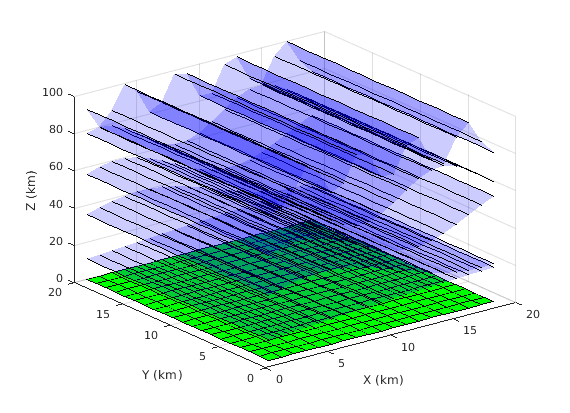
\includegraphics[width=\textwidth]{images/Lamb_model.png}
	\caption{Illustration of an atmospheric Lamb wave demonstrating the boundary conditions}
	\label{fig:1.1}
\end{figure}
%%%%%%%%%%%%%%%%%%%%%%%%%%%%%%%%%%%%%%%%%%%%%%%%%%%%%%%%%%%%%%%%%%%%%%%%%%%%%%
% Section: Approximating Atmospheric Lamb Waves
%%%%%%%%%%%%%%%%%%%%%%%%%%%%%%%%%%%%%%%%%%%%%%%%%%%%%%%%%%%%%%%%%%%%%%%%%%%%%%
\subsection{Simplifying Atmospheric Lamb Waves for a Shallow Water Approximation}\label{subsec:1.1.3}
If we consider the atmosphere as a fluid at rest this problem can be simplified immensely. A fluid at rest cannot resist any shear deformation so $\mu=0$. Notice that in this case we only consider P-waves, and the phase velocity for these waves becomes
\begin{equation}\label{eq:1.15}
	c_{p}=\sqrt{\frac{\lambda}{\rho}}. 
\end{equation}
Also in this case the Lamb wave relation is undefined. Notice this is very similar to acoustic waves. Assuming air in the atmosphere is an ideal gas, the velocity of these waves depends on temperature. This is due to the fact that
\begin{equation}\label{eq:1.16}
	\rho=\frac{P}{R_{s}T}
\end{equation}
where $R_{s}=287.052874$ $\mathrm{Jkg}^{-1}\mathrm{K}^{-1}$ is the specific gas constant for dry air, and $P$ is pressure which is also dependent on temperature $T$ for some arbitrarily small volume as stated in the ideal gas law. We will return to this idea in Chapter \ref{ch:4}. For now suppose that the atmosphere is isotropic and air is incompressible. Given these assumptions we can model waves propagating through the atmosphere as ocean waves using a shallow water approach.

The shallow water equations (SWE) are a set of hyperbolic partial differential equations (PDE)s that describe a thin layer of fluid in hydrostatic balance. This thin layer of fluid is bounded below by the bottom bathymetry and above by a free surface. The SWE are a simplification of the Navier-Stokes equations and are based on the conservation of momentum and mass. Figure \ref{fig:1.2} shows the shallow water model.
\begin{figure}[!htbp]
	\vspace{-15pt}
	\centering
	\includestandalone[width=\textwidth]{SWE}
	\caption{Illustration of a general 1D shallow water model}
	\label{fig:1.2}
\end{figure}
\pagebreak

\noindent Given the equation for hydrostatic balance 
\begin{equation}\label{eq:1.17}
	\frac{\partial P}{\partial z}=-\rho g,
\end{equation}
 where $g$ is gravity (9.81 $\mathrm{ms}^{-1}$), we can integrate both sides vertically to get
\begin{subequations}
\begin{align}
    \int_{\eta}^{b}\frac{\partial P}{\partial z}&=\int_{\eta}^{b}-\rho g dz \label{eq:1.17a}\\
    P&=-\rho g \left(b-\eta\right) \label{eq:1.17b}\\
    P&=\rho g h\label{eq:1.17c}
\end{align}
\label{eq:1.18}
\end{subequations}
since we assumed that air is incompressible $\rho=\rho_{0}$ is a constant, there is no velocity dispersion. Figure \ref{fig:1.3} below illustrates this idea.
\begin{figure}[!htbp]
	\vspace{-15pt}
	\centering
	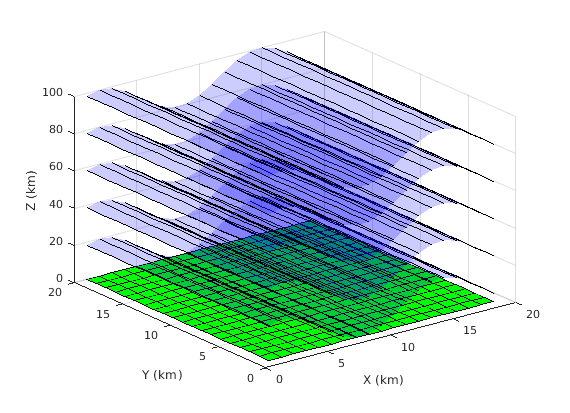
\includegraphics[width=\textwidth]{images/Lamb_isothermal_model.png}
	\caption{Illustration of an atmospheric wave with no velocity dispersion}
	\label{fig:1.3}
\end{figure}
Since there is no velocity dispersion, in two dimensions we get the following system of equations
\begin{equation}\label{eq:1.19}
	\begin{bmatrix}
		h\\
		hu\\
		hv\\
	\end{bmatrix}_{t}+\begin{bmatrix}
	uh\\
	hu^2+\frac{1}{2}gh^2\\
	uvh\\
\end{bmatrix}_{x}+\begin{bmatrix}
vh\\
uvh\\
hv^2+\frac{1}{2}gh^2\\
\end{bmatrix}_y=0
\end{equation} 
where $h(x,y,t)$ is the depth of a water column, $u(x,y,t)$ is velocity in the $x$-direction, and $v(x,y,t)$ is velocity in the $y$-direction. These waves have a phase velocity of
\begin{equation}\label{eq:1.20}
	c=\frac{\omega}{K}=\pm\sqrt{gH},
\end{equation}
given
\begin{equation}\label{eq:1.21}
\omega = \pm\sqrt{gH}K,\quad K = \sqrt{k^{2}+l^{2}}
\end{equation}
where $k$ and $l$ are the wave numbers in the $x$ and $y$ directions respectively.
%%%%%%%%%%%%%%%%%%%%%%%%%%%%%%%%%%%%%%%%%%%%%%%%%%%%%%%%%%%%%%%%%%%%%%%%%%%%%%
% Section: Previous Work
%%%%%%%%%%%%%%%%%%%%%%%%%%%%%%%%%%%%%%%%%%%%%%%%%%%%%%%%%%%%%%%%%%%%%%%%%%%%%%
\section{Previous Work}\label{sec:1.2}
The Lamb waves generated by the 2022 HTHH eruption have been successfully model by Amores et al. \cite{amores2022numerical} with the numerical ocean model, Semi-implicit Cross-scale Hydroscience Integrated System Model (SCHISM)\cite{zhang2016seamless} using the dynamic core which is based on the semi-implicit Eulerian–Lagrangian finite-element (SELFE) model\cite{zhang2008selfe}. Their simulation started with an initial perturbation being a disk of width 60 $\mathrm{km}$ and thickness of 50 $\mathrm{cm}$.

\indent Atmospheric Lamb waves have some similarities to acoustics and travel close to the speed of sound. Given the variation in temperature throughout the atmosphere, Amores et al \cite{amores2022numerical}. related the velocity at which sound waves travel through air dependent on temperature to a shallow water velocity dependent on height. They found the height at which the shallow water model must be scaled to achieve this velocity through the following equation  
\begin{equation}\label{eq:1.22}
	H=\frac{\gamma R T}{Mg}
\end{equation}
where $\gamma=1.4$ is the ratio of specific heat for air corresponding given the range of atmospheric temperatures. $R=8314.36$ $\mathrm{J\cdot kmol}^{-1}\mathrm{K}^{-1}$ is the universal gas constant, $M=28.966$ $\mathrm{kg\cdot kmol}^{-1}$ is the molecular mass for dry air, and $T$ $\mathrm{K}$ is absolute temperature. They used the tropopause starting approximately 100 $\mathrm{hPa}$ or 17 $\mathrm{km}$ at the equator as the free surface due to the temperature being constant throughout. The data used was sourced from ERA5 reanalysis, and readings from 2 $\mathrm{m}$ \cite{hersbach2018era51} above sea level were vertically averaged with readings taken from 100 $\mathrm{hPa}$ \cite{hersbach2018era52}. This vertical average was converted to a scaling height using equation \eqref{eq:1.22}. This height was then used as a bathymetry term for the associated water column. The bathymetry data was updated in the SCHISM simulation in time steps of 1 hour. Their results closely matched the observations made by satellites and other equipment referenced previously. 
%%%%%%%%%%%%%%%%%%%%%%%%%%%%%%%%%%%%%%%%%%%%%%%%%%%%%%%%%%%%%%%%%%%%%%%%%%%%%%
%
% Section: Motivation
%
%%%%%%%%%%%%%%%%%%%%%%%%%%%%%%%%%%%%%%%%%%%%%%%%%%%%%%%%%%%%%%%%%%%%%%%%%%%%%%
\section{Motivation}\label{sec:1.3}
The objective of this thesis is to implement a simplified version of the model presented by Amores et al. \cite{amores2022numerical} discussed previously in Section \ref{sec:1.3}. From the assumptions made in Sections \ref{subsec:1.1.3} to justify using a shallow water approximation we know that this model of the atmosphere must be conservative. Therefore using numerical high-resolution finite volume methods for our model is an excellent choice. Furthermore, on a large domain using methods such as adaptive mesh refinement would be extremely useful.

\indent The numerical simulation presented here uses the \fclaw library \cite{calhoun2017forestclaw}.
\fclaw is an open-source patch-based software package used to find numerical solutions for partial differential equations on a forest of quadtrees or octrees. The tree-based data structures are managed by the p4est library \cite{BursteddeWilcoxGhattas11}. The main advantage of using \fclaw is its adaptive mesh refinement capabilities.  Because the physical earth-scale domain is large relative to the Lamb wave disturbance, adaptive mesh refinement will be much more computationally efficient than working on the uniform meshes used in Amores et al. \cite{amores2022numerical},  \fclaw also makes use of high resolution solvers and other tools found in the Clawpack ecosystem \cite{mandli2016clawpack}. The primary solver featured in \fclaw is the wave propagation algorithm for solving hyperbolic partial differential equations on logically Cartesian finite volume meshes \cite{leveque2002finite}.

\indent In Chapter \ref{ch:2} of this thesis we will discuss the numerical methods used by \fclaw. In Chapter \ref{ch:3} we will present the results of a \fclaw model for the homogeneous shallow water equations at earth scale. In Chapter \ref{ch:4} a model for incorporating temperature as a bathymetry term is discussed.  


%%%%%%%%%%%%%%%%%%%%%%%%%%%%%%%%%%%%%%%%%%%%%%%%%%%%%%%%%%%%%%%%%%%%%%%%%%%%%%
%
% Chapter: Methods
%
%%%%%%%%%%%%%%%%%%%%%%%%%%%%%%%%%%%%%%%%%%%%%%%%%%%%%%%%%%%%%%%%%%%%%%%%%%%%%%

\chapter{Numerical Methods}\label{ch:2}
The goal of this thesis is to reproduce results of a simplified version of the paper from Amores et al. \cite{amores2022numerical}, discussed in the previous chapter. Our computational model is a solver for the shallow water wave equations on the sphere.  In this chapter, we will discuss the 1D shallow water wave equations and the numerical methods we use to solve these equations, including the adaptive mesh capabilities available in \fclaw.

%%%%%%%%%%%%%%%%%%%%%%%%%%%%%%%%%%%%%%%%%%%%%%%%%%%%%%%%%%%%%%%%%%%%%%%%%%%%%%
% Section: High Resolution Finite Volume Methods
%%%%%%%%%%%%%%%%%%%%%%%%%%%%%%%%%%%%%%%%%%%%%%%%%%%%%%%%%%%%%%%%%%%%%%%%%%%%%%
\section{High Resolution Finite Volume Methods}\label{sec:2.1}
One of the solvers available in \fclaw uses finite-volume methods to find numerical solutions for hyperbolic PDEs \cite{leveque2002finite}. Specifically, \fclaw uses a high resolution wave propagation algorithm for linear and nonlinear conservative hyperbolic systems \cite{leveque1997wave}. Consider the one dimensional case of an equation in conservative form
\begin{equation}\label{eq:2.1}
    \mathbf{q}_{t}+f(\mathbf{q})_{x}=0,
\end{equation}
where $\mathbf{q}$ is a vector of conserved quantities that are dependent on space and time, and $f$ is a flux function dependant on $\mathbf{q}$. We define a cell centered mesh over the one dimensional domain $x\in\left[a,b\right]$ for $a,b\in\mathbb{R}$ such that the cell edges are given by $C_{i}=\left[x_{i-\frac{1}{2}},x_{i+\frac{1}{2}}\right]$. 
Rearranging equation \eqref{eq:2.1}
\begin{equation*}
    \frac{\partial}{\partial t}q(x,t)=-\frac{\partial}{\partial x}f(q(x,t))
\end{equation*}
then integrating both sides over a cell and dividing through by its length $\Delta x$
\begin{equation}\label{eq:2.2}
    \frac{1}{\Delta x}\int_{x_{i-\frac{1}{2}}}^{x_{i+\frac{1}{2}}}\frac{\partial}{\partial t}q(x,t)dx=-\frac{1}{\Delta x}\int_{x_{i-\frac{1}{2}}}^{x_{i+\frac{1}{2}}}\frac{\partial}{\partial x} f(q(x,t))dx
\end{equation}
leads to an evolution formula for the average value in cell $C_i$. Using the divergence theorem and pulling $\partial /\partial t$ out of the integral on the left hand side, we get
\begin{equation}\label{eq:2.3}
    \frac{\partial}{\partial t}\left(\frac{1}{\Delta x}\int_{x_{i-\frac{1}{2}}}^{x_{i+\frac{1}{2}}}q(x,t)dx\right)=\frac{1}{\Delta x}\left[f\left(q\left(x_{i-\frac{1}{2}},t\right)\right)-f\left(q\left(x_{i+\frac{1}{2}},t\right)\right)\right]
\end{equation} This integral expresses the change in the cell average as a  difference of the fluxes through the boundaries. We can solve this as a differential equation in time to get the exact evolution formula
\begin{equation}\label{eq:2.4}
\begin{aligned}
     \frac{1}{\Delta x}\int_{x_{i-\frac{1}{2}}}^{x_{i+\frac{1}{2}}}q(x,t_{n+1})dx&=\frac{1}{\Delta x}\int_{x_{i-\frac{1}{2}}}^{x_{i+\frac{1}{2}}}q(x,t_{n})dx\\&-\frac{1}{\Delta x}\left[\int_{t_{n}}^{t_{n+1}}f\left(q\left(x_{i+\frac{1}{2}},t\right)\right)dt-\int_{t_{n}}^{t_{n+1}}f\left(q\left(x_{i-\frac{1}{2}},t\right)\right)dt\right].
     \end{aligned}
\end{equation}
We can replace this with a discrete evolution formula
\begin{equation}\label{eq:2.5}
    Q_{i}^{n+1}=Q_{i}^{n}-\frac{\Delta t}{\Delta x}\left[F_{i+\frac{1}{2}}^{n}-F_{i-\frac{1}{2}}^{n}\right]
\end{equation}
where $Q_i$ is the cell average given by
\begin{equation}\label{eq:2.6}
Q_i^n = \frac{1}{\Delta x}\int_{x_{i-\frac{1}{2}}}^{x_{i+\frac{1}{2}}}q(x,t_{n})dx
\end{equation}
and  $F_{i-\frac{1}{2}}$ is an approximation to the integral 
\begin{equation}\label{eq:2.7}
F_{i-\frac12}^n \approx 
\int_{t_{n}}^{t_{n+1}}f\left(q\left(x_{i-\frac{1}{2}},t\right)\right)dt.
\end{equation}

%%%%%%%%%%%%%%%%%%%%%%%%%%%%%%%%%%%%%%%%%%%%%%%%%%%%%%%%%%%%%%%%%%%%%%%%%%%%%%
% Section: riemann problems
%%%%%%%%%%%%%%%%%%%%%%%%%%%%%%%%%%%%%%%%%%%%%%%%%%%%%%%%%%%%%%%%%%%%%%%%%%%%%%
\subsection{Riemann problems}\label{subsec:2.1.1}
Since we are working with a discrete evolution formula the values at the cell interfaces are initially undefined and the integral in \eqref{eq:2.4} cannot be computed exactly. The challenge is to approximate the fluxes in \eqref{eq:2.7} through other means. The Riemann problem is a fundamental part of numerical finite volume methods, and consists of a conservative equation paired with some special initial data. Suppose there is a jump at $x=0$, then a Riemann problem for a hyperbolic conservation law would be of the form
\begin{equation}\label{eq:2.8}
\begin{split}
    &q_{t}+f(q)_{x}=0\\
    &\text{subject to}\\
    &q(x,0)=\begin{cases}
        q_{\ell}\quad& x<0\\
        q_{r}\quad&x>0\\
    \end{cases}
    \end{split}
\end{equation}
where $q_{\ell}$ and $q_{r}$ are the average values of the left and right neighboring cells respectively. By solving this problem we can gather information about the state in between the two cells. This information can then be used to calculate the numerical fluxes and evolve a finite volume scheme over a time step. Riemann problems for linear systems can be solved by means of eigendecomposition as shown in the next section.

%%%%%%%%%%%%%%%%%%%%%%%%%%%%%%%%%%%%%%%%%%%%%%%%%%%%%%%%%%%%%%%%%%%%%%%%%%%%%%
% Section: Wave Propagation Algorithm for Linear system
%%%%%%%%%%%%%%%%%%%%%%%%%%%%%%%%%%%%%%%%%%%%%%%%%%%%%%%%%%%%%%%%%%%%%%%%%%%%%%
 \section{Wave Propagation Algorithm for Linear systems}\label{sec:2.2}
 For linear hyperbolic systems we can express equation \eqref{eq:2.1} as
 \begin{equation}\label{eq:2.9}
     \mathbf{q}_{t}+\mathbf{A}\mathbf{q}_{x}=0     
 \end{equation}
 where $\mathbf{A}$ is a $m\times m$ matrix. The system is hyperbolic if $\mathbf{A}$ is diagonalizable with real eigenvalues. Then $\mathbf{A}$ can be written as 
 \begin{equation}\label{eq:2.10}
     \mathbf{A}=\mathbf{R}\mathbf{\Lambda} \mathbf{R}^{-1}
 \end{equation}
 where $\mathbf{R}=[\mathbf{r}^{1},\mathbf{r}^{2},\dots,\mathbf{r}^{m}]$ is the set of eigenvectors, and $\mathbf{\Lambda}=\mbox{diag}(\lambda^{1},\lambda^{2},\dots,\lambda^{m})$ is the diagonal matrix of the corresponding eigenvalues which are also the characteristic wave speeds. We define the characteristic variables of the system as
 \begin{equation}\label{eq:2.11}
     \omega(\mathbf{x},\mathbf{t})=\mathbf{R}^{-1}\mathbf{q}.
 \end{equation}
 We can decouple the system into a set of $m$ scalar equations, multiplying \eqref{eq:2.10} by $\mathbf{R}^{-1}$ 
\begin{equation}\label{eq:2.12}
\mathbf{R}^{-1}\mathbf{q}_{t}+\mathbf{R}^{-1}\left(\mathbf{R}\mathbf{\Lambda} \mathbf{R}^{-1}\right)\mathbf{q}_{x}=0    
\end{equation}
leads to
\begin{equation}\label{eq:2.13}
    \omega^{p}_{t}+\lambda^{p}\omega^{p}_{x}=0
\end{equation}
for $p=1,2,\dots,m$. Given some special initial data 
\begin{equation}\label{eq:2.14}
    \omega(\mathbf{x},0)=\mathbf{R}^{-1}\mathbf{q}(\mathbf{x},0)
\end{equation}
the solution to this set of equations is given by 
\begin{equation}\label{eq:2.15}
    \omega^{p}(x,t)=\omega(x-\lambda^{p}t,0).
\end{equation}
Then for any time $t$ we can see that
\begin{equation}\label{eq:2.16}
\mathbf{q}(\mathbf{x},\mathbf{t}) = \mathbf{R}\omega(\mathbf{x},\mathbf{t}) = \sum_{p=1}^{m} \omega^p(x,t)\mathbf{r}^p
\end{equation}
is a linear combination of eigenvectors. 
If the initial conditions are given by piecewise constant data in the Riemann problem \eqref{eq:2.14}, then the solution can be decomposed into a series of jumps
\begin{equation}\label{eq:2.17}
    \mathbf{q}_{\ell}-\mathbf{q}_{r}=\sum_{p=1}^{m}\left(\omega^{p}(x_{i},t)-\omega^{p}(x_{i-1},t)\right)\mathbf{r}^{p},
\end{equation}
In the Wave Propagation Algorithm \cite{leveque2002finite}, we define waves as scalar multiple of eigenvectors 
\begin{equation}\label{eq:2.18}
    \mathbf{\mathcal{W}}_{i-\frac{1}{2}}^{p}\equiv\alpha^{p}\mathbf{r}^{p}
\end{equation}
where $\alpha = \left(\omega^{p}(x_{i},t)-\omega^{p}(x_{i-1},t)\right)$.
Fluctuations at the cell interfaces are defined as
\begin{equation}\label{eq:2.19}
    \mathbf{A}^{+}\Delta \mathbf{Q}_{i-\frac{1}{2}} \equiv \sum_{p=1}^{m}\left(\lambda^{p}\right)^{+}\mathbf{\mathcal{W}}_{i-\frac{1}{2}}^{p}\quad\text{and}\quad \mathbf{A}^{-}\Delta \mathbf{Q}_{i-\frac{1}{2}} \equiv \sum_{p=1}^{m}\left(\lambda^{p}\right)^{-}\mathbf{\mathcal{W}}_{i-\frac{1}{2}}^{p}
\end{equation}
where $\left(\lambda^{p}\right)^{+}=\max\left(\lambda^p,0\right)$ and  $\left(\lambda^{p}\right)^{-}=\min\left(\lambda^p,0\right)$. Then using these values along with equation \eqref{eq:2.5}
\begin{equation}\label{eq:2.20}
    \begin{split}
    \mathbf{Q}_{i}^{n+1}&=\mathbf{Q}_{i}^{n}-\frac{\Delta t}{\Delta x}\left[\sum_{p=1}^{m}\left(\lambda^{p}\right)^{+}\mathbf{\mathcal{W}}_{i-\frac{1}{2}}^{p}+\sum_{p=1}^{m}\left(\lambda^{p}\right)^{-}\mathbf{\mathcal{W}}_{i+\frac{1}{2}}^{p}\right]\\
    &=\mathbf{Q}_{i}^{n}-\frac{\Delta t}{\Delta x}\left[\mathbf{A}^{+}\Delta \mathbf{Q}_{i-\frac{1}{2}}+\mathbf{A}^{-}\Delta \mathbf{Q}_{i+\frac{1}{2}}\right]
    \end{split}
\end{equation} 
we can evolve the system in time. The solution to the Riemann problem for the special initial conditions can now be expressed in terms of eigenvectors and eigenvalues
\begin{equation}\label{eq:2.21}
\mathbf{q}(\mathbf{x},\mathbf{t})=
    \begin{cases}
     \mathbf{q}_{\ell} \quad &\frac{x}{t}<x-\lambda^{p}t\\
     \mathbf{q}_{\ell}+\alpha^{p}\mathbf{r}^{p} \quad &x-\lambda^{p}t<\frac{x}{t}<x+\lambda^{p}t\\
     \mathbf{q}_r\quad &\frac{x}{t}>x+\lambda^{p}t
    \end{cases},
\end{equation}
 While this is a first order approximation we can add on a correction terms defined as 
\begin{equation}\label{eq:2.22}
    \mathbf{\tilde{F}}_{i-\frac{1}{2}} \equiv \frac{1}{2}\sum_{p=1}^{m}|\lambda^{p}|\left(1-\frac{\Delta t}{\Delta x}|\lambda^{p}|\right)\mathbf{\mathcal{W}}_{i-\frac{1}{2}}^{p}
\end{equation}
to the update formula
\begin{equation}\label{eq:2.23}
    \mathbf{Q}_{i}^{n+1}=\mathbf{Q}_{i}^{n}-\frac{\Delta t}{\Delta x}\left[\mathbf{A}^{+}\Delta \mathbf{Q}_{i-\frac{1}{2}}+\mathbf{A}^{-}\Delta \mathbf{Q}_{i+\frac{1}{2}}\right]-\frac{\Delta t}{\Delta x}\left[\mathbf{\tilde{F}_{i+\frac{1}{2}}}-\mathbf{\tilde{F}_{i-\frac{1}{2}}}\right]
\end{equation} 
and get second order accuracy.
%%%%%%%%%%%%%%%%%%%%%%%%%%%%%%%%%%%%%%%%%%%%%%%%%%%%%%%%%%%%%%%%%%%%%%%%%%%%%%
% Section: Example: The Linearized Shallow Water Equations
%%%%%%%%%%%%%%%%%%%%%%%%%%%%%%%%%%%%%%%%%%%%%%%%%%%%%%%%%%%%%%%%%%%%%%%%%%%%%%
\subsection{Example: The Linearized Shallow Water Equations}\label{subsec:2.2.1}
Consider the one dimensional linearized shallow water equations
\begin{equation}\label{eq:2.24}
    \begin{bmatrix}
        h\\
        u
    \end{bmatrix}_{t}+\begin{bmatrix}
        U&H\\
        g&U
    \end{bmatrix}\begin{bmatrix}
        h\\
        u
    \end{bmatrix}_{x}=0
\end{equation}
where $H$ is the average height deviation from the bottom to the free surface and $U$ is the average initial velocity. The eigenvectors for this system are
$$\mathbf{r}^{1}=\begin{bmatrix}
    -\sqrt{gH}\\
    g
\end{bmatrix},\quad \mathbf{r}^{2}=\begin{bmatrix}
    \sqrt{gH}\\
    g
\end{bmatrix}$$
and have the corresponding eigenvalues or wave speeds are $\lambda^{1}=U-\sqrt{gH}$, $\lambda^{2}=U+\sqrt{gH}$. Solving for the characteristic variables
\begin{equation}\label{eq:2.25}
    \begin{bmatrix}
        -\sqrt{gH}&\sqrt{gH}\\
        g&g
    \end{bmatrix}\begin{bmatrix}
        \alpha^{1}\\
        \alpha^{2}
    \end{bmatrix}=\begin{bmatrix}
        h_{r}-h_{\ell}\\
        u_{r}-u_{\ell}
    \end{bmatrix}
\end{equation}
results in 
\begin{equation}\label{eq:2.26}
    \begin{bmatrix}
        \alpha^{1}\\
        \alpha^{2}
    \end{bmatrix}=\frac{1}{2gH}\begin{bmatrix}
        -\sqrt{gH}&H\\
        \sqrt{gH}&H
    \end{bmatrix}\begin{bmatrix}
        h_{r}-h_{\ell}\\
        u_{r}-u_{\ell}
    \end{bmatrix}.
\end{equation}
From here we can arrive at the solution to the Riemann problem
\begin{equation}\label{eq:2.27}
    \mathbf{q}(x,t)=\begin{cases}
        \mathbf{q}_{\ell}&\frac{x}{t}< U-\sqrt{gH}\\
        \mathbf{q}_{\ell}+\alpha^1\mathbf{r}^{1}\quad&U-\sqrt{gH}<\frac{x}{t}<U+\sqrt{gH}\\
        \mathbf{q}_{r}&\frac{x}{t}>U+\sqrt{gH}
    \end{cases}.
\end{equation}

%%%%%%%%%%%%%%%%%%%%%%%%%%%%%%%%%%%%%%%%%%%%%%%%%%%%%%%%%%%%%%%%%%%%%%%%%%%%%%
% Section: Wave Propagation algorithm for Nonlinear Systems
%%%%%%%%%%%%%%%%%%%%%%%%%%%%%%%%%%%%%%%%%%%%%%%%%%%%%%%%%%%%%%%%%%%%%%%%%%%%%%
\section{Wave Propagation Algorithm for Nonlinear Systems}\label{sec:2.3}
For nonlinear systems the same approach can be used. However, we want to replace the nonlinear problem 
\begin{equation*}
    \mathbf{q}_{t}+f(\mathbf{q})_{x}=0
\end{equation*}
with some linear problem that approximates $f(\mathbf{q})$ for a small neighborhood $\mathbf{\widehat{q}}$ around the cell interfaces. We can write the nonlinear system in quasi-linear form as
\begin{equation}\label{eq:2.28}
    \mathbf{q}_{t}+\mathbf{A}(\mathbf{\widehat{q}})\mathbf{q}_{x}=0
\end{equation}
where 
\begin{equation}\label{eq:2.29}
    \mathbf{A}=\frac{\partial f}{\partial \mathbf{q}}
\end{equation} is the flux Jacobian matrix. Since $\mathbf{A}$ depends on $\mathbf{q}$ we must choose the appropriate values of $\mathbf{q}$ at which to evaluate $\mathbf{A}$ and its eigenvalues. This is done using Roe-averaged values which are found using the conservation properties of $\mathbf{A}$. For example the non-linear shallow water equations shown in Section \ref{subsec:2.3.1} have the Roe-averaged values of 
\begin{equation}\label{eq:2.30}
\widehat{h} = \frac{h_{r}+h_{\ell}}{2}
\end{equation}
and 
\begin{equation}\label{eq:2.31}
    \widehat{u}=\frac{u_{r}\sqrt{h_{r}}+u_{\ell}\sqrt{h_{\ell}}}{\sqrt{h_{r}}+\sqrt{h_{\ell}}}.
\end{equation}
We proceed by finding the eigenvectors and eigenvalues of $\mathbf{A}$ as in Section \ref{sec:2.2}. Then we can solve the Riemann problem at the cell interfaces just as we did for a linear system.

%%%%%%%%%%%%%%%%%%%%%%%%%%%%%%%%%%%%%%%%%%%%%%%%%%%%%%%%%%%%%%%%%%%%%%%%%%%%%%
% Section: Example: The Nonlinear Shallow Water Equations
%%%%%%%%%%%%%%%%%%%%%%%%%%%%%%%%%%%%%%%%%%%%%%%%%%%%%%%%%%%%%%%%%%%%%%%%%%%%%%
\subsection{Example: The Nonlinear Shallow Water Equations }\label{subsec:2.3.1}
 For example consider the one dimensional 
 nonlinear shallow water equations 
\begin{equation}\label{eq:2.32}
    \begin{bmatrix}
    h\\
    hu\\
    \end{bmatrix}_{t}+\begin{bmatrix}
        uh\\
        hu^2+\frac{1}{2}gh^2\\
    \end{bmatrix}_{x}=0
\end{equation}
here 
\begin{equation}\label{eq:2.33}
    \mathbf{q}=\begin{bmatrix}
        h\\
        hu\\
    \end{bmatrix}
    =\begin{bmatrix}
        q^1\\
        q^2\\
    \end{bmatrix}
\end{equation}
and 
\begin{equation}\label{eq:2.34}
    f(\mathbf{q})=\begin{bmatrix}
        hu\\
        hu^2+\frac{1}{2}gh^2\\
    \end{bmatrix}
    =\begin{bmatrix}
        q^2\\
        \frac{(q^2)^2}{q^1}+\frac{1}{2}g(q^1)^2\\
    \end{bmatrix}.
\end{equation}
For the system \eqref{eq:2.32} the flux Jacobian matrix is
\begin{equation}\label{eq:2.35}
    \mathbf{A}=f'(\mathbf{q})=\begin{bmatrix}
        0&1\\
        -u^2+gh&2u\\
    \end{bmatrix}
    =\begin{bmatrix}
        0&1\\
        -\left(\frac{q^2}{q^1}\right)^2+gq^1&2\frac{q^2}{q^1}\\
    \end{bmatrix}.
\end{equation}
Since in this case $\mathbf{A}$ depends on $\mathbf{q}$ we must use the Roe-averaged values
\begin{equation}\label{eq:2.36}
    \mathbf{\hat{q}}=\begin{bmatrix}
        \widehat{h}\\
        \widehat{h}\widehat{u}
    \end{bmatrix}
\end{equation}
where
\begin{equation}\label{eq:2.37}
    \widehat{h}=\frac{h_{r}+h_{\ell}}{2}\quad\text{and}\quad\widehat{u}=\frac{u_{r}\sqrt{h_{r}}+u_{\ell}\sqrt{h_{\ell}}}{\sqrt{h_{r}}+\sqrt{h_{\ell}}}.
\end{equation}
Then we have
\begin{equation}\label{eq:2.38}
f'(\mathbf{\widehat{q}})=\begin{bmatrix}
        0&1\\
        -\widehat{u}^2+g\widehat{h}&2\widehat{u}\\
    \end{bmatrix}
\end{equation}
this matrix has the corresponding eigenvectors 
\begin{equation}\label{eq:2.39}
    \mathbf{\widehat{r}}^{1}=\begin{bmatrix}
        1\\
        \widehat{u}-\sqrt{g\widehat{h}}\\
    \end{bmatrix}\quad\text{and}\quad
    \mathbf{\widehat{r}}^{2}=\begin{bmatrix}
        1\\
        \widehat{u}+\sqrt{g\widehat{h}}\\
    \end{bmatrix}
\end{equation} with eigenvalues of $\widehat{\lambda}^1=\widehat{u}-\sqrt{g\widehat{h}}$ and $\widehat{\lambda}^2=\widehat{u}+\sqrt{g\widehat{h}}$. Having found the characteristics of the system we can now find a solution to the Riemann problem at a cell interface the same way as demonstrated in Section \ref{subsec:2.2.1}.
%%%%%%%%%%%%%%%%%%%%%%%%%%%%%%%%%%%%%%%%%%%%%%%%%%%%%%%%%%%%%%%%%%%%%%%%%%%%%%
% Section: Adaptive Mesh Refinement
%%%%%%%%%%%%%%%%%%%%%%%%%%%%%%%%%%%%%%%%%%%%%%%%%%%%%%%%%%%%%%%%%%%%%%%%%%%%%%
\section{Adaptive Mesh Refinement}\label{sec:2.4}
Adaptive mesh refinement (AMR) is a way of changing the spacing of grid points on a given domain, a grid within in a grid. This allows for resolution to be high in a region of the domain that includes relevant parts of the solution while keeping other regions of the domain at a relatively low resolution. This is accomplished by grouping cells into sections known as patches. Patches are then refined based on their proximity to the areas of interest for the given solution. The figure \ref{fig:2.1} below illustrates this idea and shows three levels of refinement. The use of AMR prevents unnecessary calculations that would occur on a static grid, and improves computational speed. 
\begin{figure}[!htbp]
	\centering
\includestandalone[width=0.4\textwidth]{AMR}
\caption{Adaptive Mesh Refinement}
\label{fig:2.1}
\end{figure}
\noindent 
%%%%%%%%%%%%%%%%%%%%%%%%%%%%%%%%%%%%%%%%%%%%%%%%%%%%%%%%%%%%%%%%%%%%%%%%%%%%%%
% Section: Surface Mapping and Resolution
%%%%%%%%%%%%%%%%%%%%%%%%%%%%%%%%%%%%%%%%%%%%%%%%%%%%%%%%%%%%%%%%%%%%%%%%%%%%%%
\subsection{Surface Mapping and Resolution}\label{subsec:2.4.1}
To use AMR with \fclaw requires a computational mesh grid. However, this presents a problem when we want to find a solution on a sphere. The problem occurs as all of the grid-lines converge at the poles if we use an equally spaced latitude and longitude grid. To avoid this problem we have used a cubed sphere mapping \cite{calhoun2008logically}. All calculations regarding AMR and resolution presented here are based on this mapping. With a domain as large as the planet earth AMR will be beneficial as several computations are required at the boundary of every mesh cell. Not only is this very resource intensive, but it takes time. With AMR we can capture events that are only a few kilometers in diameter while at the same time keeping the rest of the globe at a resolution better measured with degrees of latitude and longitude. 

We can determine the required resolution using AMR for a square patch of side length $\mathcal{P}$ with at least $\mathcal{M}$ mesh cells across a region of interest. The circumference of the earth is 
\begin{equation}\label{eq:2.40}
    C=2\pi R
\end{equation}
where $R=6378100$ $\mathrm{m}$. The number of mesh cells around the equator on the cubed sphere is given by
\begin{equation}\label{eq:2.41}
    \mathcal{M}_{equator}=4\left(2^{\ell}\mathcal{P}\right)
\end{equation}
where $2^{\ell}\mathcal{P}$ is the effective patch resolution. The resolution at equator is given by
\begin{equation}\label{eq:2.42}
    h_{equator}=\frac{C}{\mathcal{M}_{equator}},
\end{equation}
and similarly we can calculate the resolution required for a region of interest
\begin{equation}\label{eq:2.43}
    h_{required}=\frac{\mathcal{D}}{\mathcal{M}}
\end{equation}
where $\mathcal{D}$ is the diameter of the region of interest in kilometers.
To calculate the needed level of refinement we can set \eqref{eq:2.42} equal to \eqref{eq:2.43} and solve for $\ell$ which results in the following formula
\begin{equation}\label{eq:2.44}
	\ell=\log_{2}\left(\frac{\pi R \mathcal{M}}{2\mathcal{P}\mathcal{D}}\right).
\end{equation}
 We will use
\begin{equation}\label{eq:2.45}
	\mathcal{D}=\mathcal{M}\left(\frac{2\pi R}{4\mathcal{P}2^{\ell}}\right).
\end{equation} 
to compute the minimum diameter of a perturbation that we are able to capture at a given level of refinement. Table \ref{tbl:2.1} shows the size of the perturbations each level of refinement is able to capture assuming a patch size of $\mathcal{P}=32$, and at least $\mathcal{M}=6$ mesh cells across the diameter $\mathcal{D}$ of the region. 
\begin{table}[!htbp]
    \vspace{-3pt}
	\caption{Resolution of AMR assuming a patch size of $\mathcal{P}=32$}
	\label{tbl:2.1}
	\begin{center}
			\setlength{\tabcolsep}{3pt}
			\begin{tabular}{l|l|l|l}
					\hline
					    Refinement Level&Minimum Event Diameter [$\mathrm{km}$]&\# Mesh Cells&Resolution [$\mathrm{km}$]\\
					$\ell$&$\mathcal{D}$&$\mathcal{M}$&$h$\\
					 \hline \hline
					0 & 1879 & 6 &  313.1\\
					\hline
					1 & 940 & 6 & 156.5\\
					\hline
					2 & 470 & 6 & 78.3\\
					\hline
					3 & 235 & 6 & 39.1\\
					\hline
					4 & 118 & 6 & 19.6\\ 
					\hline
					5 & 59 & 6 & 9.8\\
					 \hline
				\end{tabular}
		\end{center}
\end{table}

\noindent Using table \ref{tbl:2.1} as a guide, figure \ref{fig:2.2} below created with the Climate Data Toolbox for MATLAB \cite{greene2019climate}, demonstrates the advantages of AMR on a large domain such as earth by contrasting it with same the refinement everywhere.
\begin{figure}[!htbp]
\centering
\begin{subfigure}{\textwidth}
  \centering
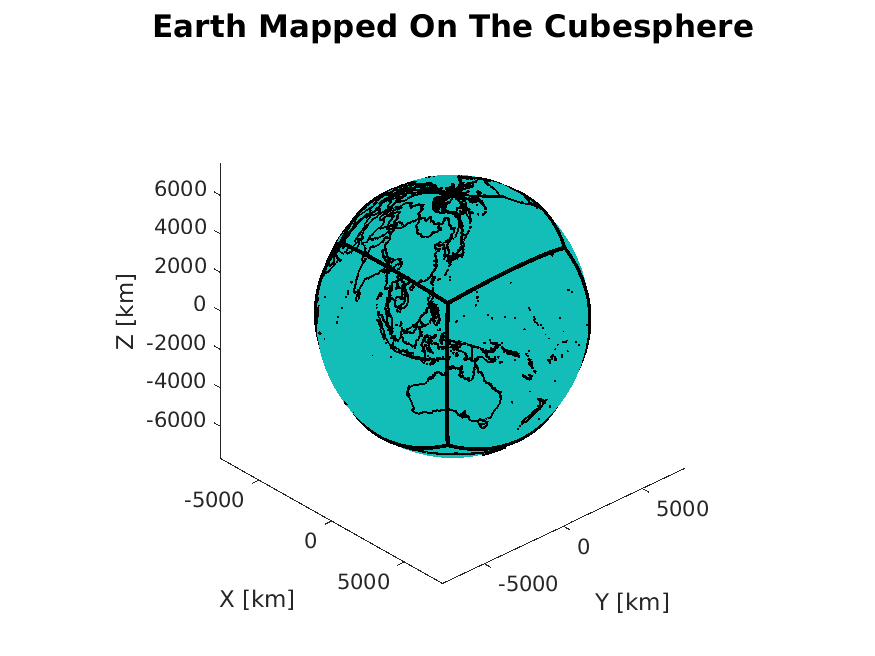
\includegraphics[height=0.27\textheight,clip=True,trim=1.8cm 0.6cm 2.6cm 2.6cm]{images/earth_cube.png}
  \caption{Earth mapped on the cubed sphere}
\end{subfigure}
\begin{subfigure}{\textwidth}
  \centering
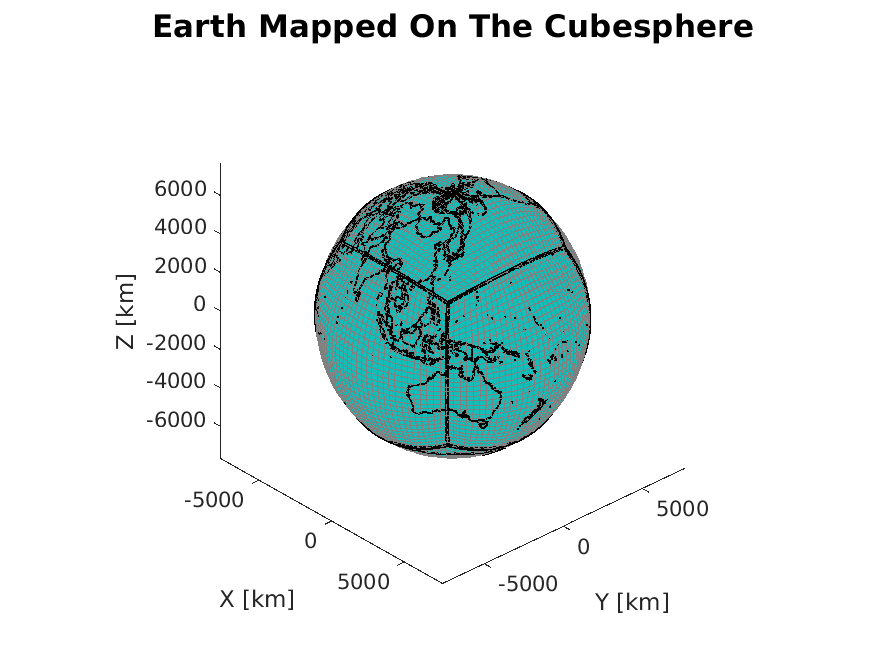
\includegraphics[height=0.27\textheight,clip=True,trim=1.8cm 0.6cm 2.6cm 2.6cm]{images/earth_cube_mesh.png}
  \caption{Earth mapped on the cubed sphere with a mesh grid}
\end{subfigure}
\medskip
\begin{subfigure}{\textwidth}
  \centering
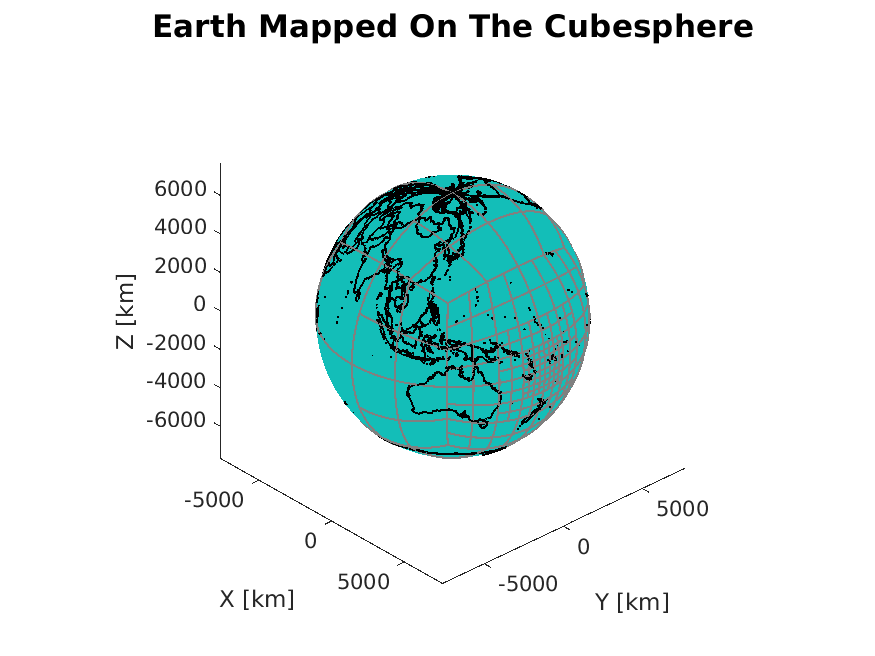
\includegraphics[height=0.27\textheight,clip=True,trim=1.8cm 0.6cm 2.6cm 2.6cm]{images/earth_cube_amr.png}
  \caption{Earth mapped on the cubed sphere with AMR (Levels 0-5)}
\end{subfigure}
\caption{Resolution and surface mapping}
\label{fig:2.2}
\end{figure}



%%%%%%%%%%%%%%%%%%%%%%%%%%%%%%%%%%%%%%%%%%%%%%%%%%%%%%%%%%%%%%%%%%%%%%%%%%%%%%
%
% Chapter: Results
%
%%%%%%%%%%%%%%%%%%%%%%%%%%%%%%%%%%%%%%%%%%%%%%%%%%%%%%%%%%%%%%%%%%%%%%%%%%%%%%
\chapter{Results For the Homogeneous Shallow Water Equations at Earth Scale}\label{ch:3}
Before attempting to solve the more complicated problem proposed in Section \ref{sec:1.2} by Amores et al \cite{amores2022numerical}. we want to verify that we get a reasonable result with a similar but much simpler problem. The speed of waves in the shallow water equations are dependent on height. With the height of the tropopause at about 17 $\mathrm{km}$ near the equator, we want to verify that we can numerically approximate a wave given these extreme depths. Here we will show the results for the homogeneous shallow water equations at earth scale. 
%%%%%%%%%%%%%%%%%%%%%%%%%%%%%%%%%%%%%%%%%%%%%%%%%%%%%%%%%%%%%%%%%%%%%%%%%%%%%%
% Section: Initial Conditions and Parameters
%%%%%%%%%%%%%%%%%%%%%%%%%%%%%%%%%%%%%%%%%%%%%%%%%%%%%%%%%%%%%%%%%%%%%%%%%%%%%%
\section{Initial Conditions and Parameters For the Homogeneous Shallow Water Equations at Earth Scale}\label{sec:3.1}
 The simulation starts with an initial perturbation of a cylinder that is 60 km wide and 50 cm thick at the 100 $\mathrm{hPa}$ taken to be approximately 17 $\mathrm{km}$. To capture this event we used AMR up to level 5 as described in table \ref{tbl:2.1}, a refinement threshold of 0.001 $\mathrm{m}$, and a coarsening threshold of 0.0005 $\mathrm{m}$. A windless atmosphere is assumed, as well as a constant temperature throughout. The topography of the earth is not taken into account. Figure \ref{fig:3.1} below illustrates the described initial conditions.
\begin{figure}[!htbp]
	\centering
	\includestandalone[width=\textwidth]{IC_flat}
	\caption{Initial conditions and the shallow water model assuming a flat bottom}
	\label{fig:3.1}
\end{figure}
%%%%%%%%%%%%%%%%%%%%%%%%%%%%%%%%%%%%%%%%%%%%%%%%%%%%%%%%%%%%%%%%%%%%%%%%%%%%%%
% Section: Homogeneous Results at earth scale
%%%%%%%%%%%%%%%%%%%%%%%%%%%%%%%%%%%%%%%%%%%%%%%%%%%%%%%%%%%%%%%%%%%%%%%%%%%%%%
\section{Homogeneous Results at Earth Scale}\label{sec:3.2}
    Here we present the results of our simulation given the initial conditions described previously in Section \ref{sec:3.1} using the numerical methods discussed in Section \ref{sec:2.3}. Figure \ref{fig:3.2} below shows the result of the homogeneous model as described in Section \ref{sec:3.1} over a 24 hour time period. 
    Computations took 1.3 hours on 18 cores of a Dell XPS 9520 with a 12th Gen Intel core i7-12700 $\mathrm{H}$ processor and 32 $\mathrm{gb}$ ram. 
\begin{figure}[!htbp]
\centering
\begin{subfigure}{\textwidth}
  \centering
  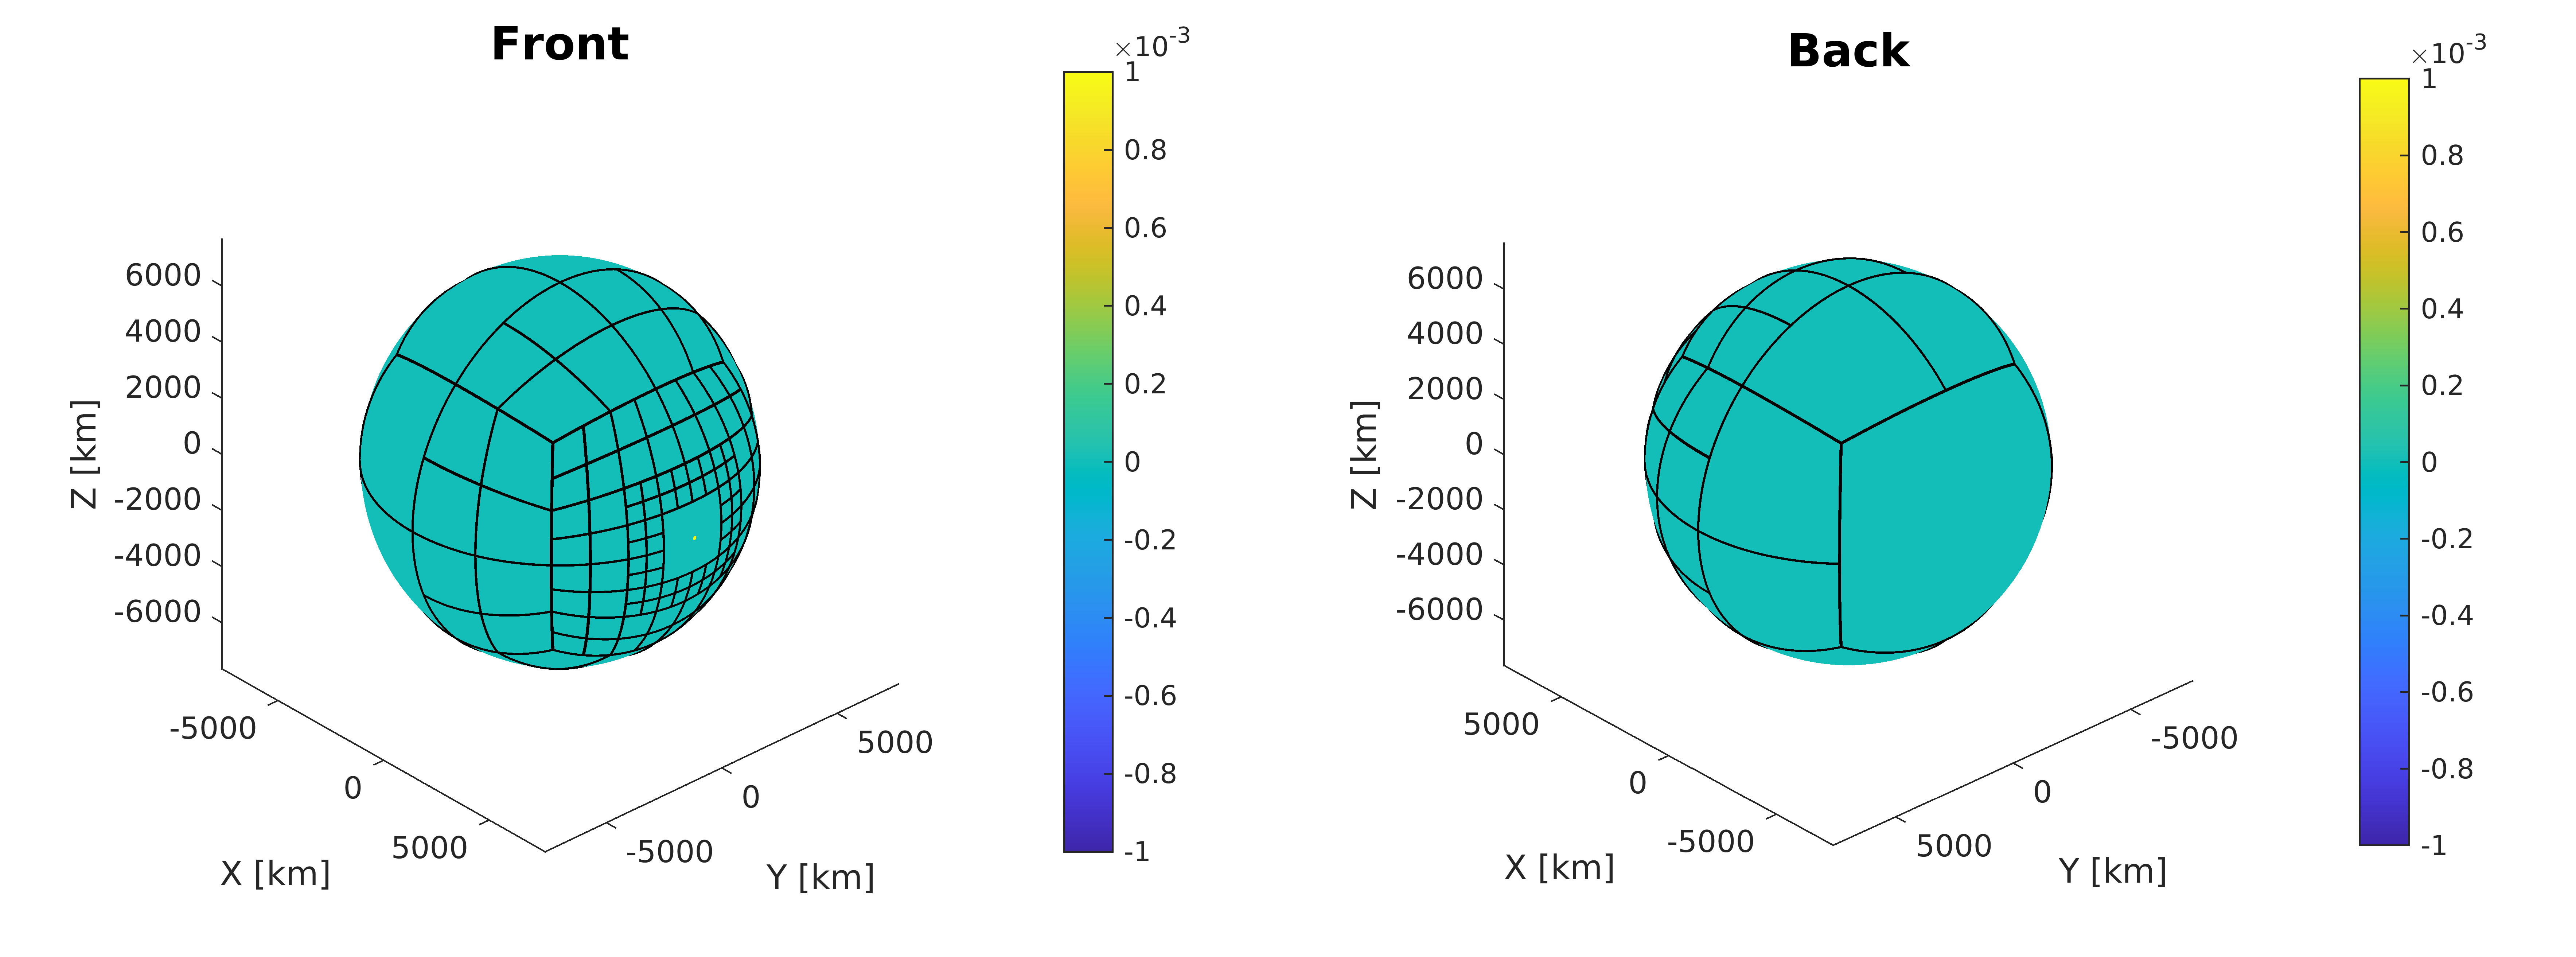
\includegraphics[width=0.95\textwidth,clip=True,trim=4cm 0cm 4cm 0cm]{images/ideal/ideal_0.png}
  \caption{Time: 0 hours }
\end{subfigure}
\caption{Solution: 15 January 2022, 04:00 $\mathrm{UTC}$ - 16 January 2022, 04:00 $\mathrm{UTC}$}
\end{figure}

\begin{figure}[!htbp]\ContinuedFloat
\vspace{-15pt}
\centering
\begin{subfigure}{\textwidth}
  \centering
  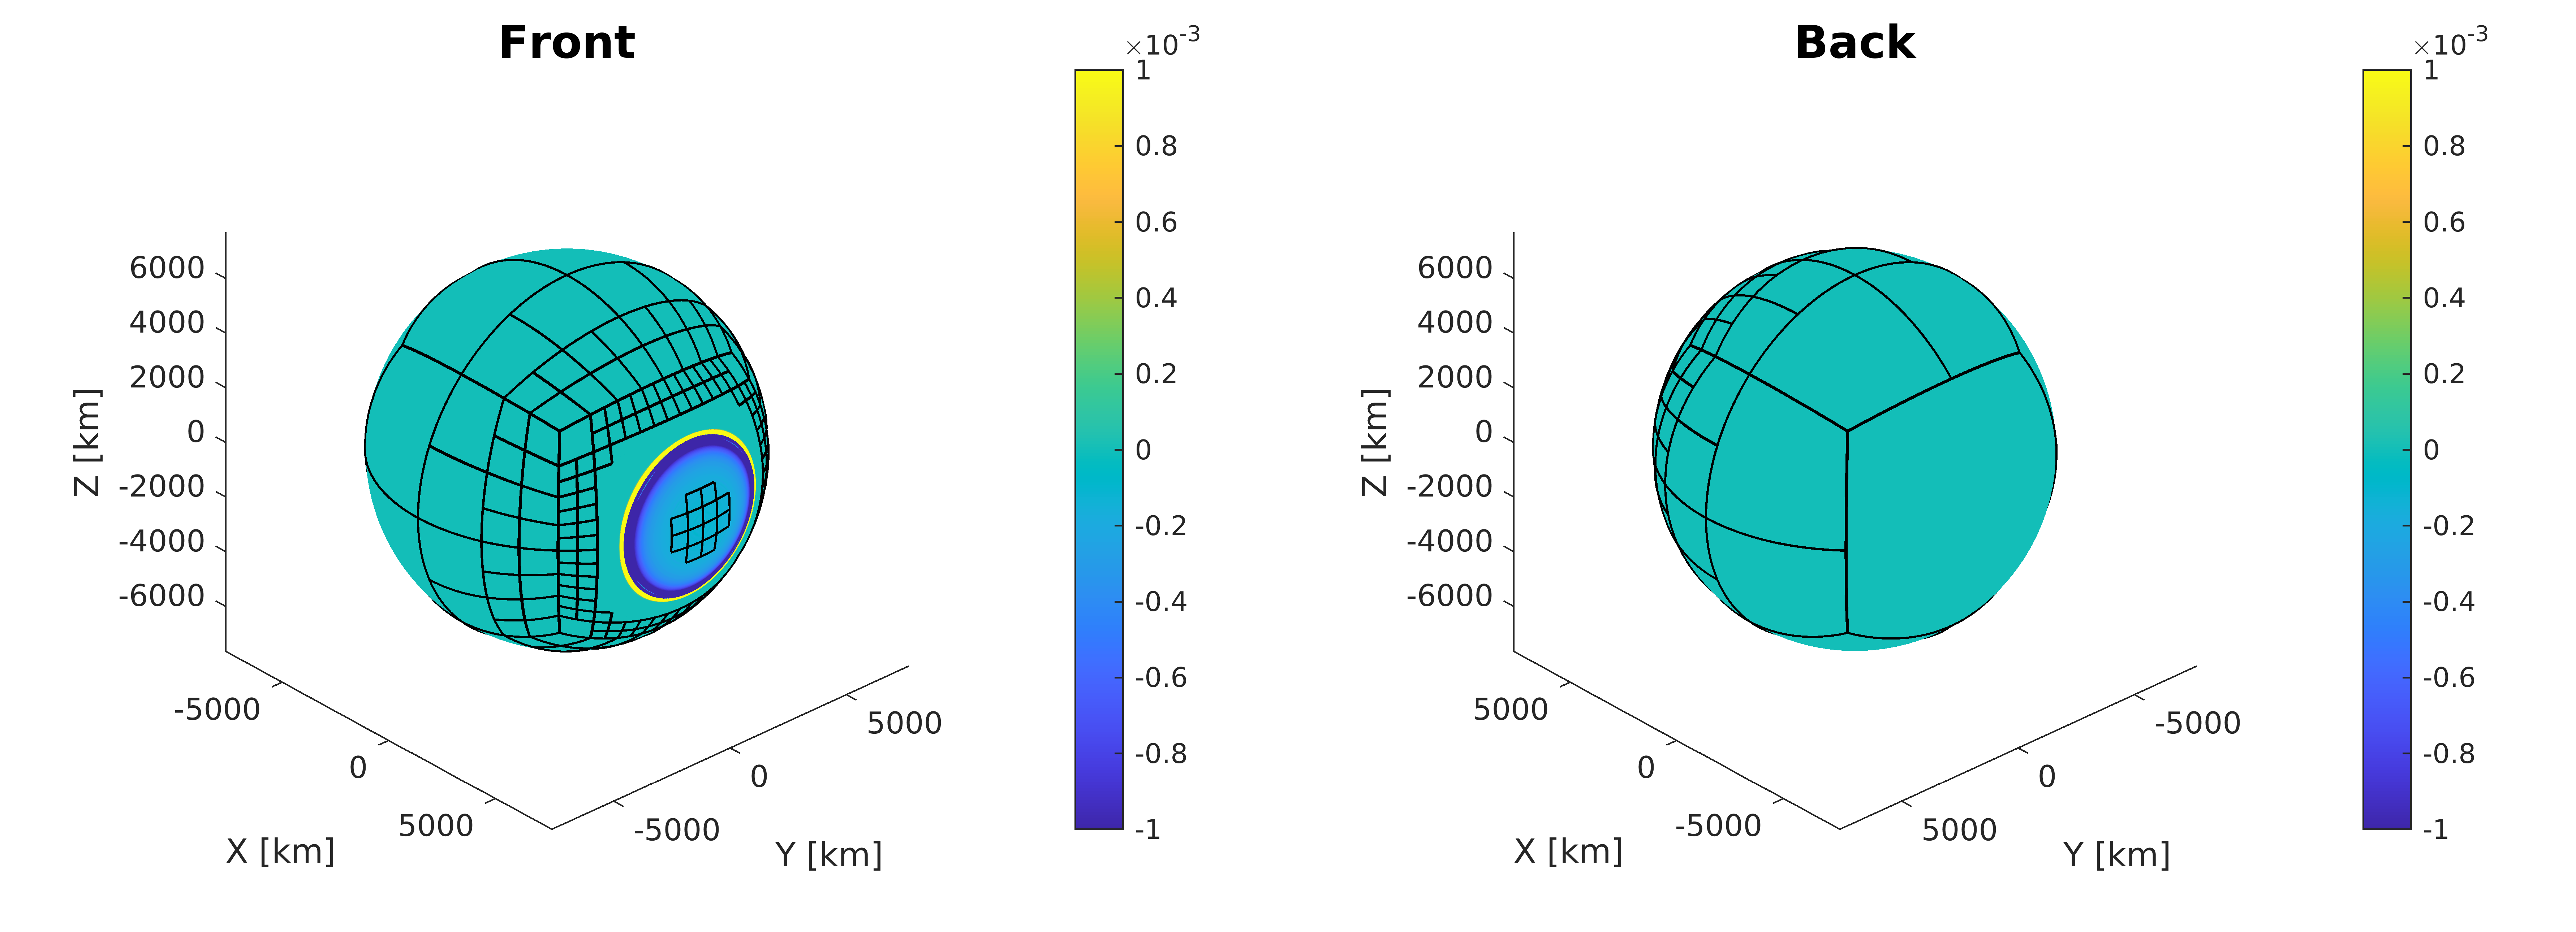
\includegraphics[width=0.95\textwidth,clip=True,trim=4cm 0cm 4cm 0cm]{images/ideal/ideal_4.png}
  \caption{Time: 2 hours }
\end{subfigure}

\medskip

\begin{subfigure}{\textwidth}
  \centering
  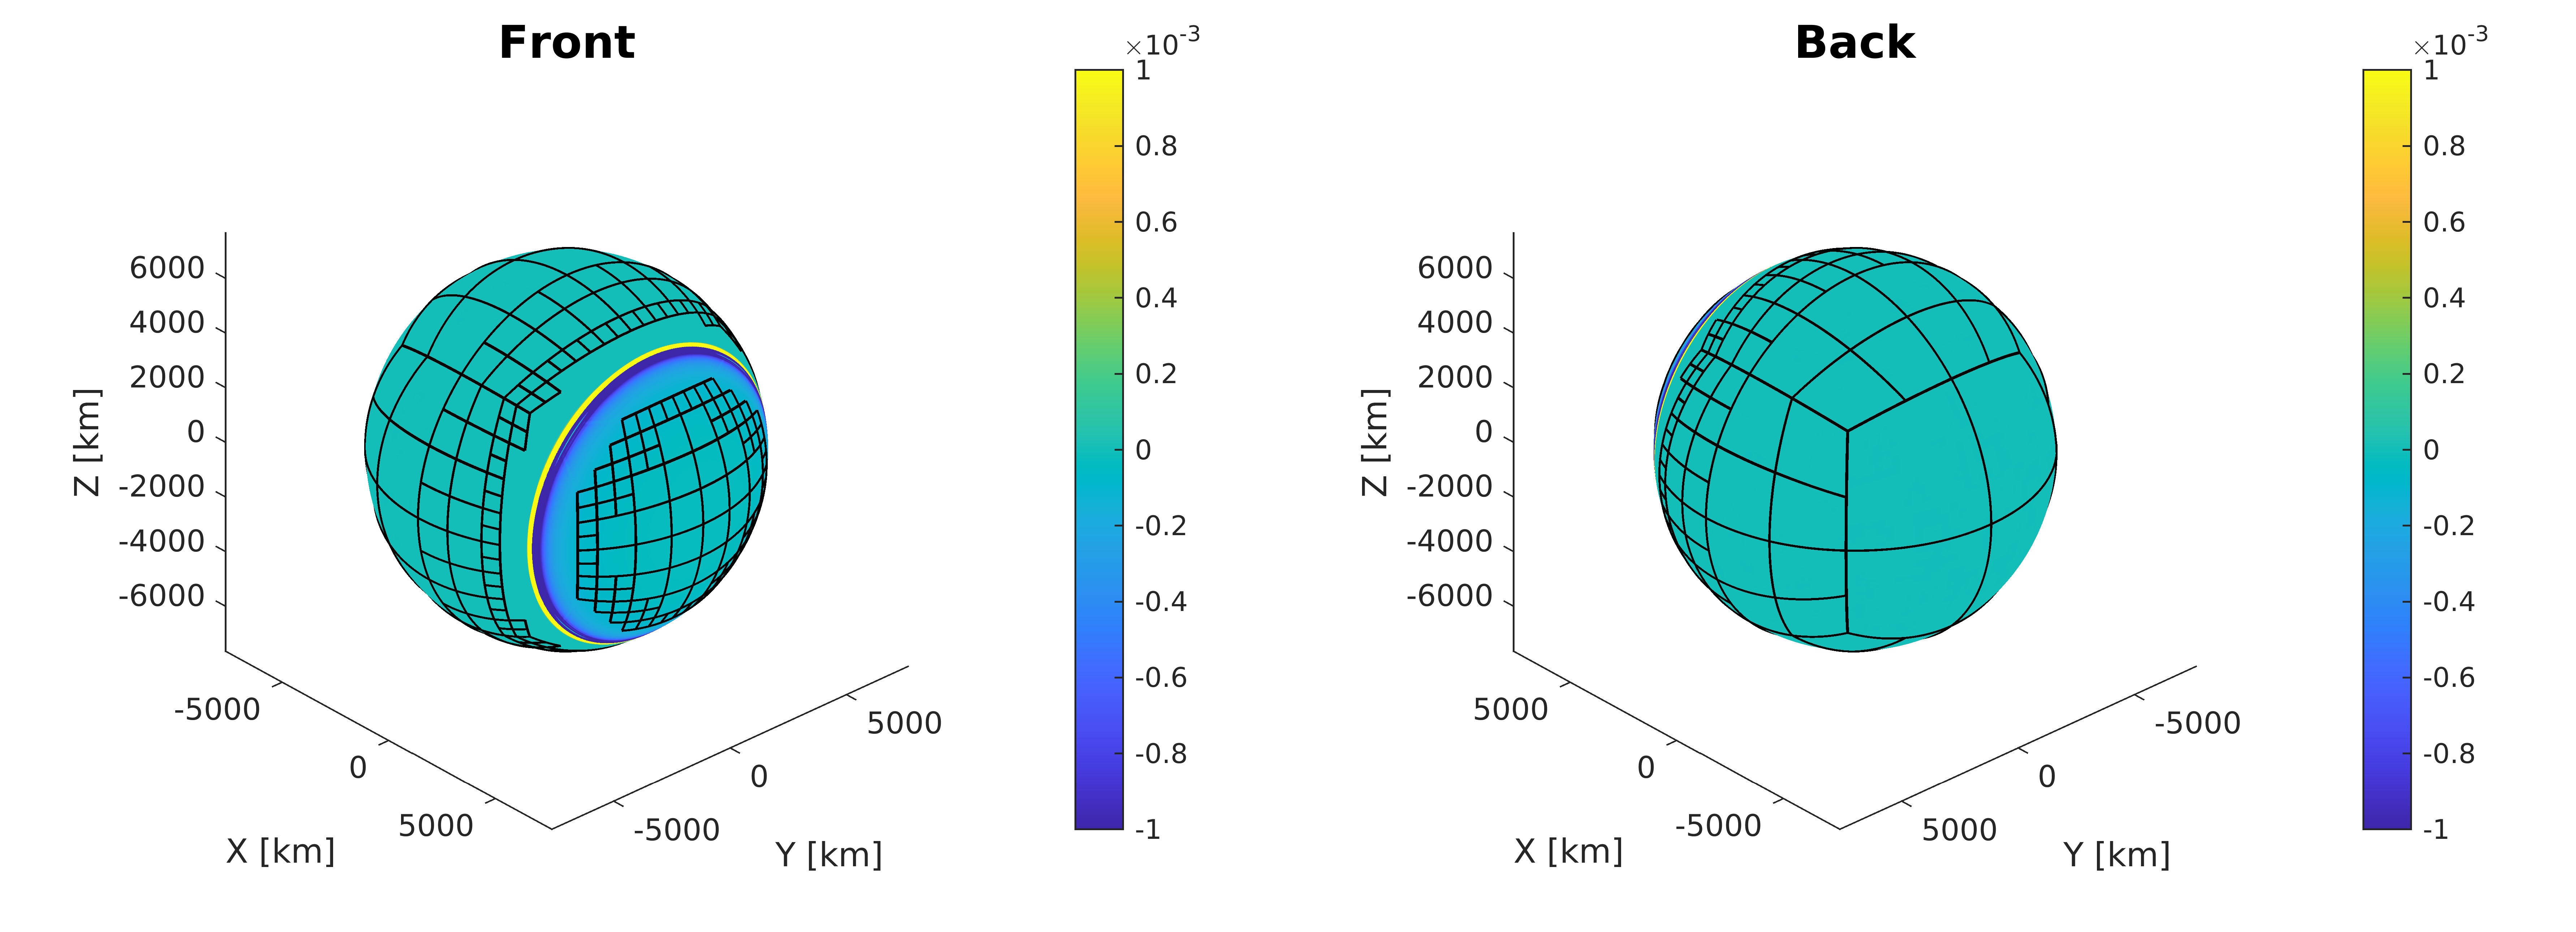
\includegraphics[width=0.95\textwidth,clip=True,trim=4cm 0cm 4cm 0cm]{images/ideal/ideal_8.png}
  \caption{Time: 4 hours }
\end{subfigure}

\medskip

\begin{subfigure}{\textwidth}
  \centering
  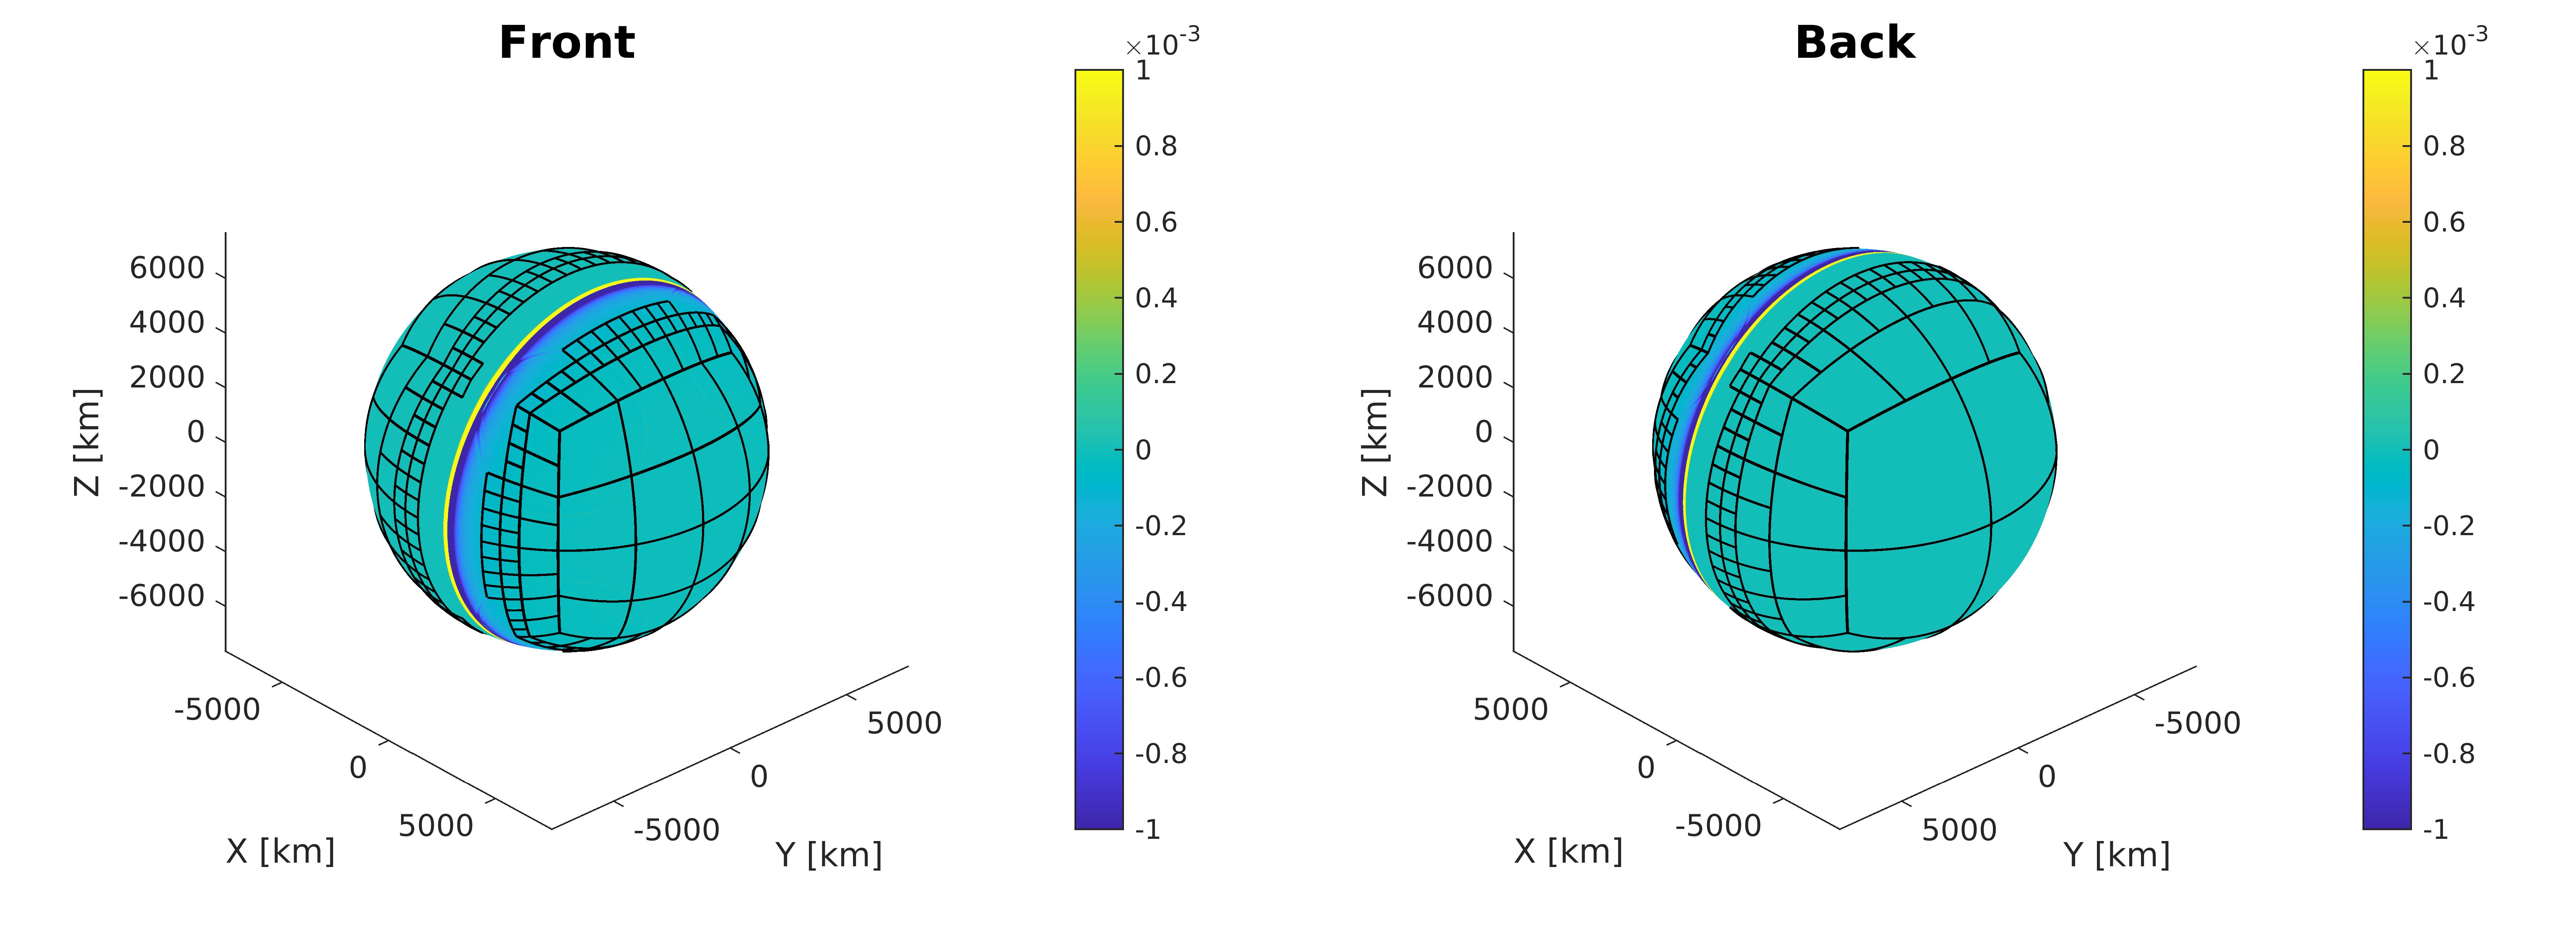
\includegraphics[width=0.95\textwidth,clip=True,trim=4cm 0cm 4cm 0cm]{images/ideal/ideal_12.png}
  \caption{Time: 6 hours }
\end{subfigure}

\caption{Solution: 15 January 2022, 04:00 $\mathrm{UTC}$ - 16 January 2022, 04:00 $\mathrm{UTC}$}
\end{figure}

\medskip

\begin{figure}[!htbp]\ContinuedFloat
\vspace{-15pt}
\centering

\begin{subfigure}{\textwidth}
  \centering
  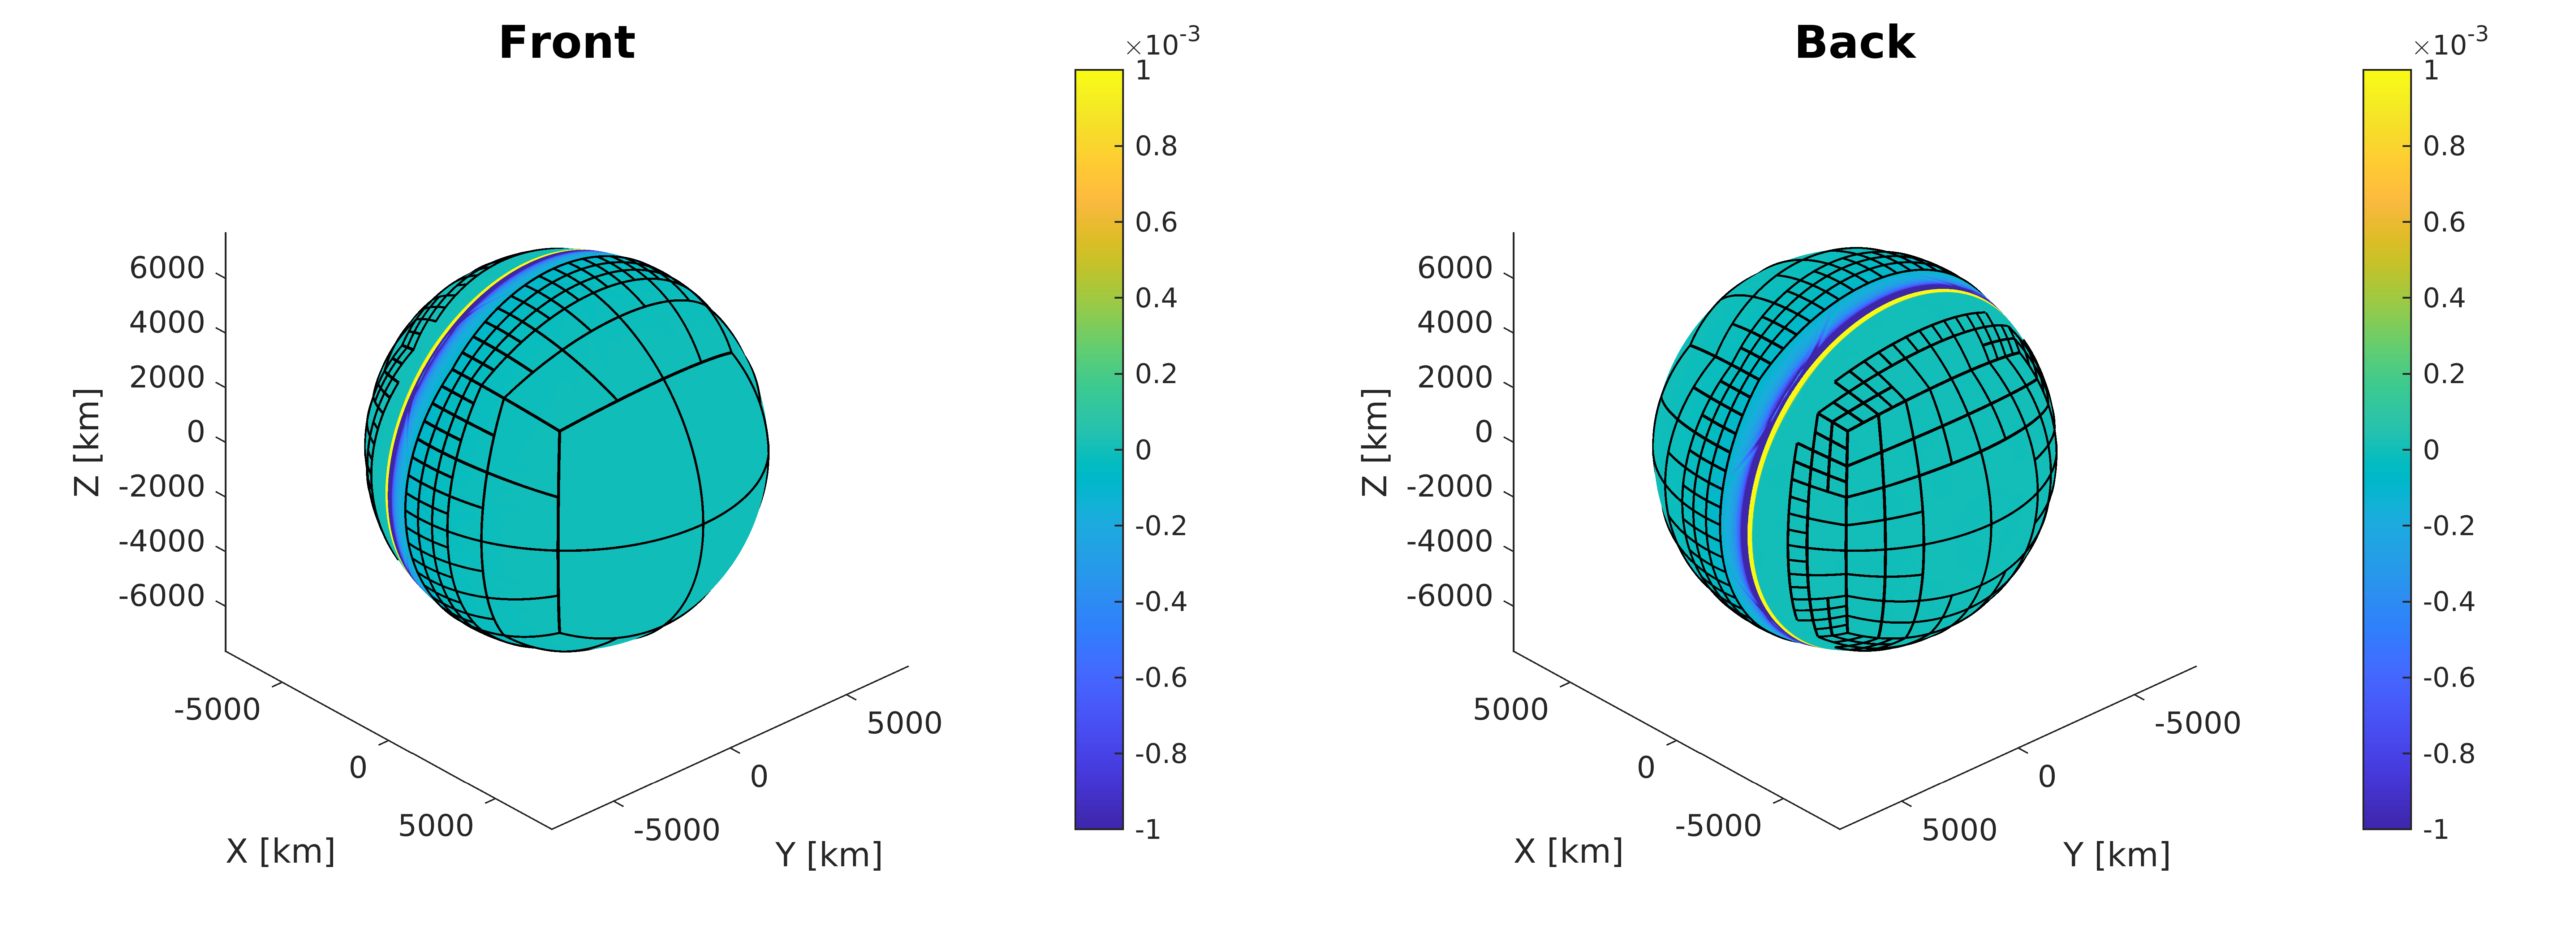
\includegraphics[width=0.95\textwidth,clip=True,trim=4cm 0cm 4cm 0cm]{images/ideal/ideal_16.png}
  \caption{Time: 8 hours }
\end{subfigure}

\medskip

\begin{subfigure}{\textwidth}
  \centering
  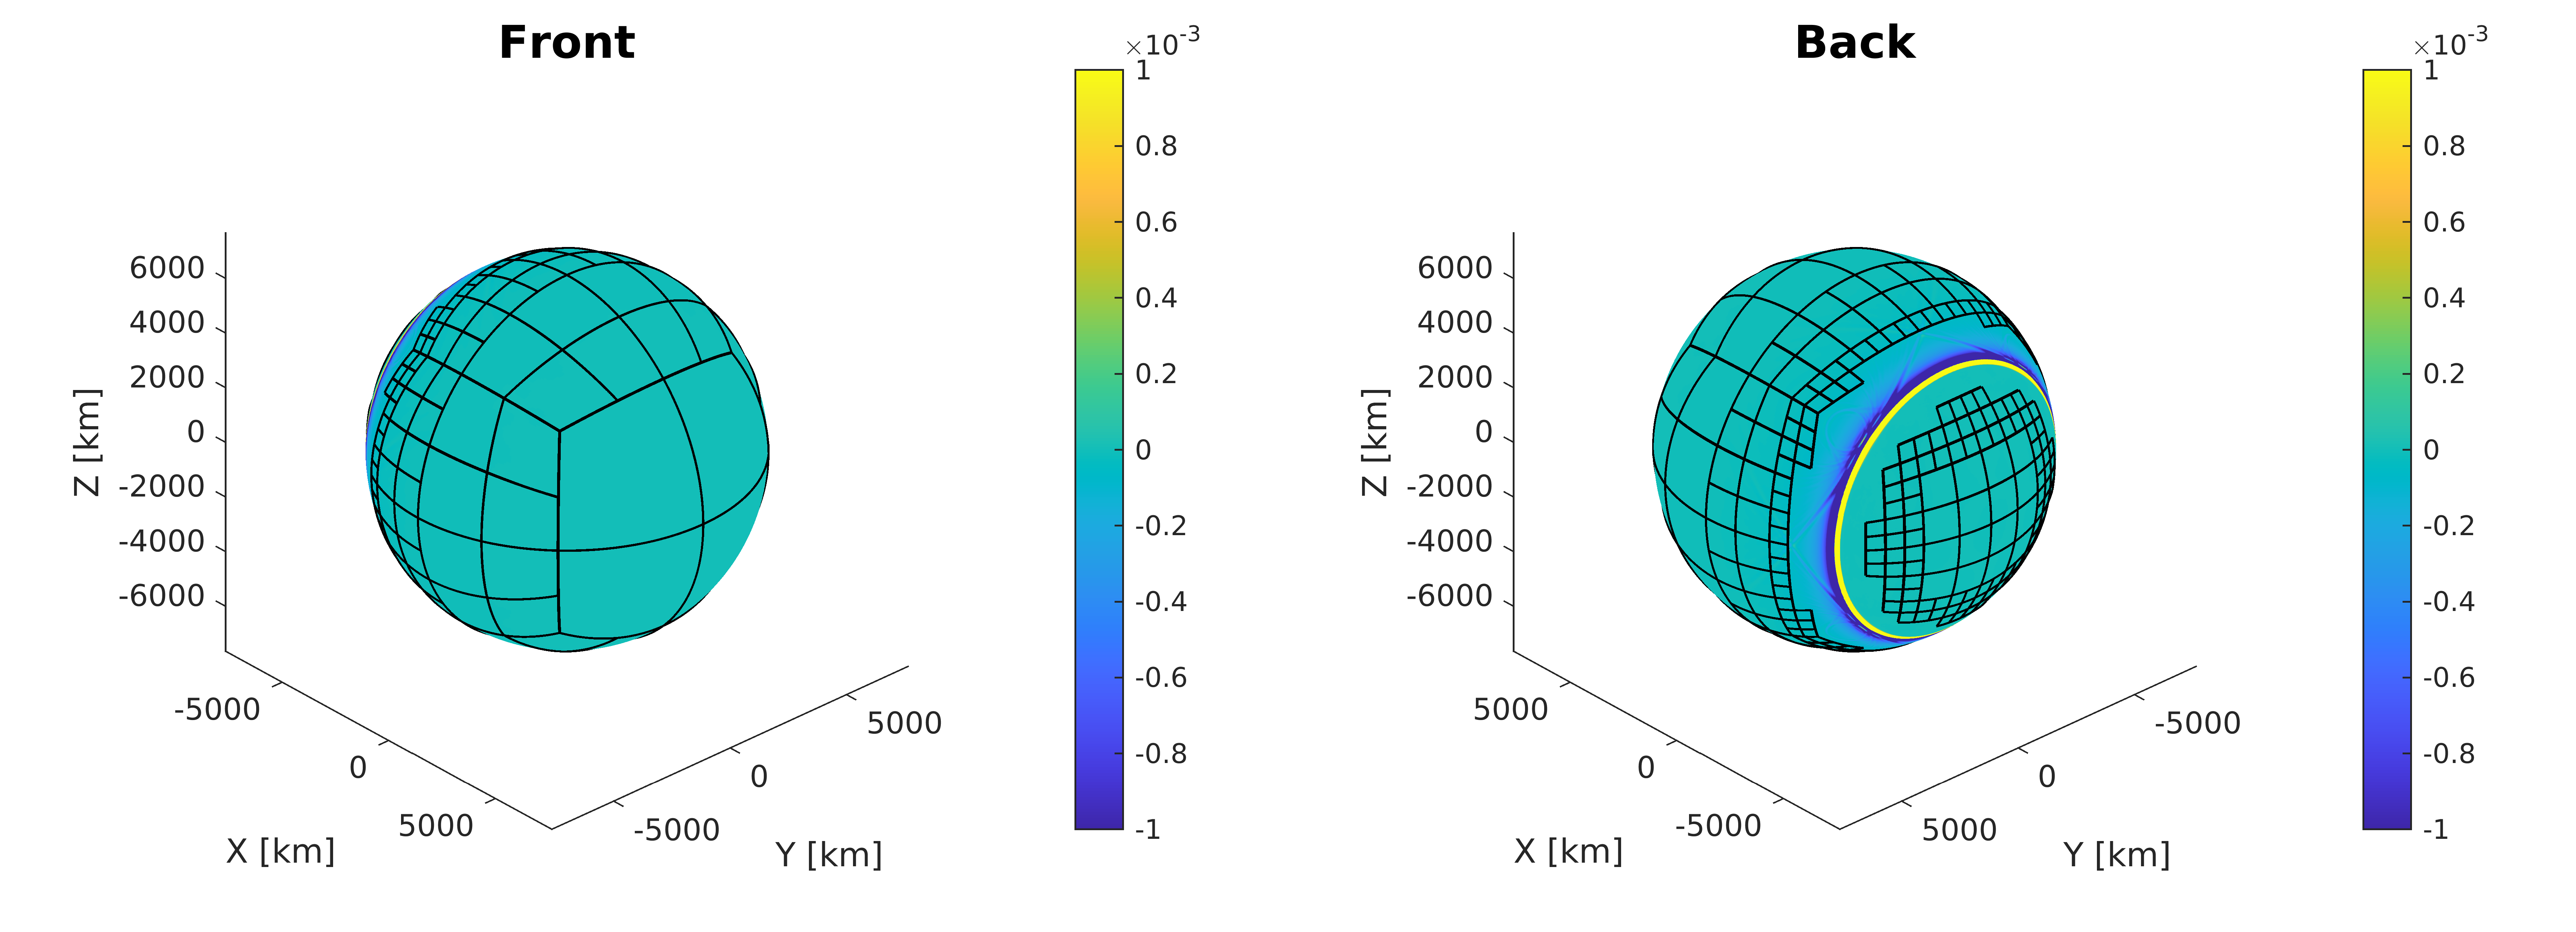
\includegraphics[width=0.95\textwidth,clip=True,trim=4cm 0cm 4cm 0cm]{images/ideal/ideal_20.png}
  \caption{Time: 10 hours }
\end{subfigure}

\medskip

\begin{subfigure}{\textwidth}
  \centering
  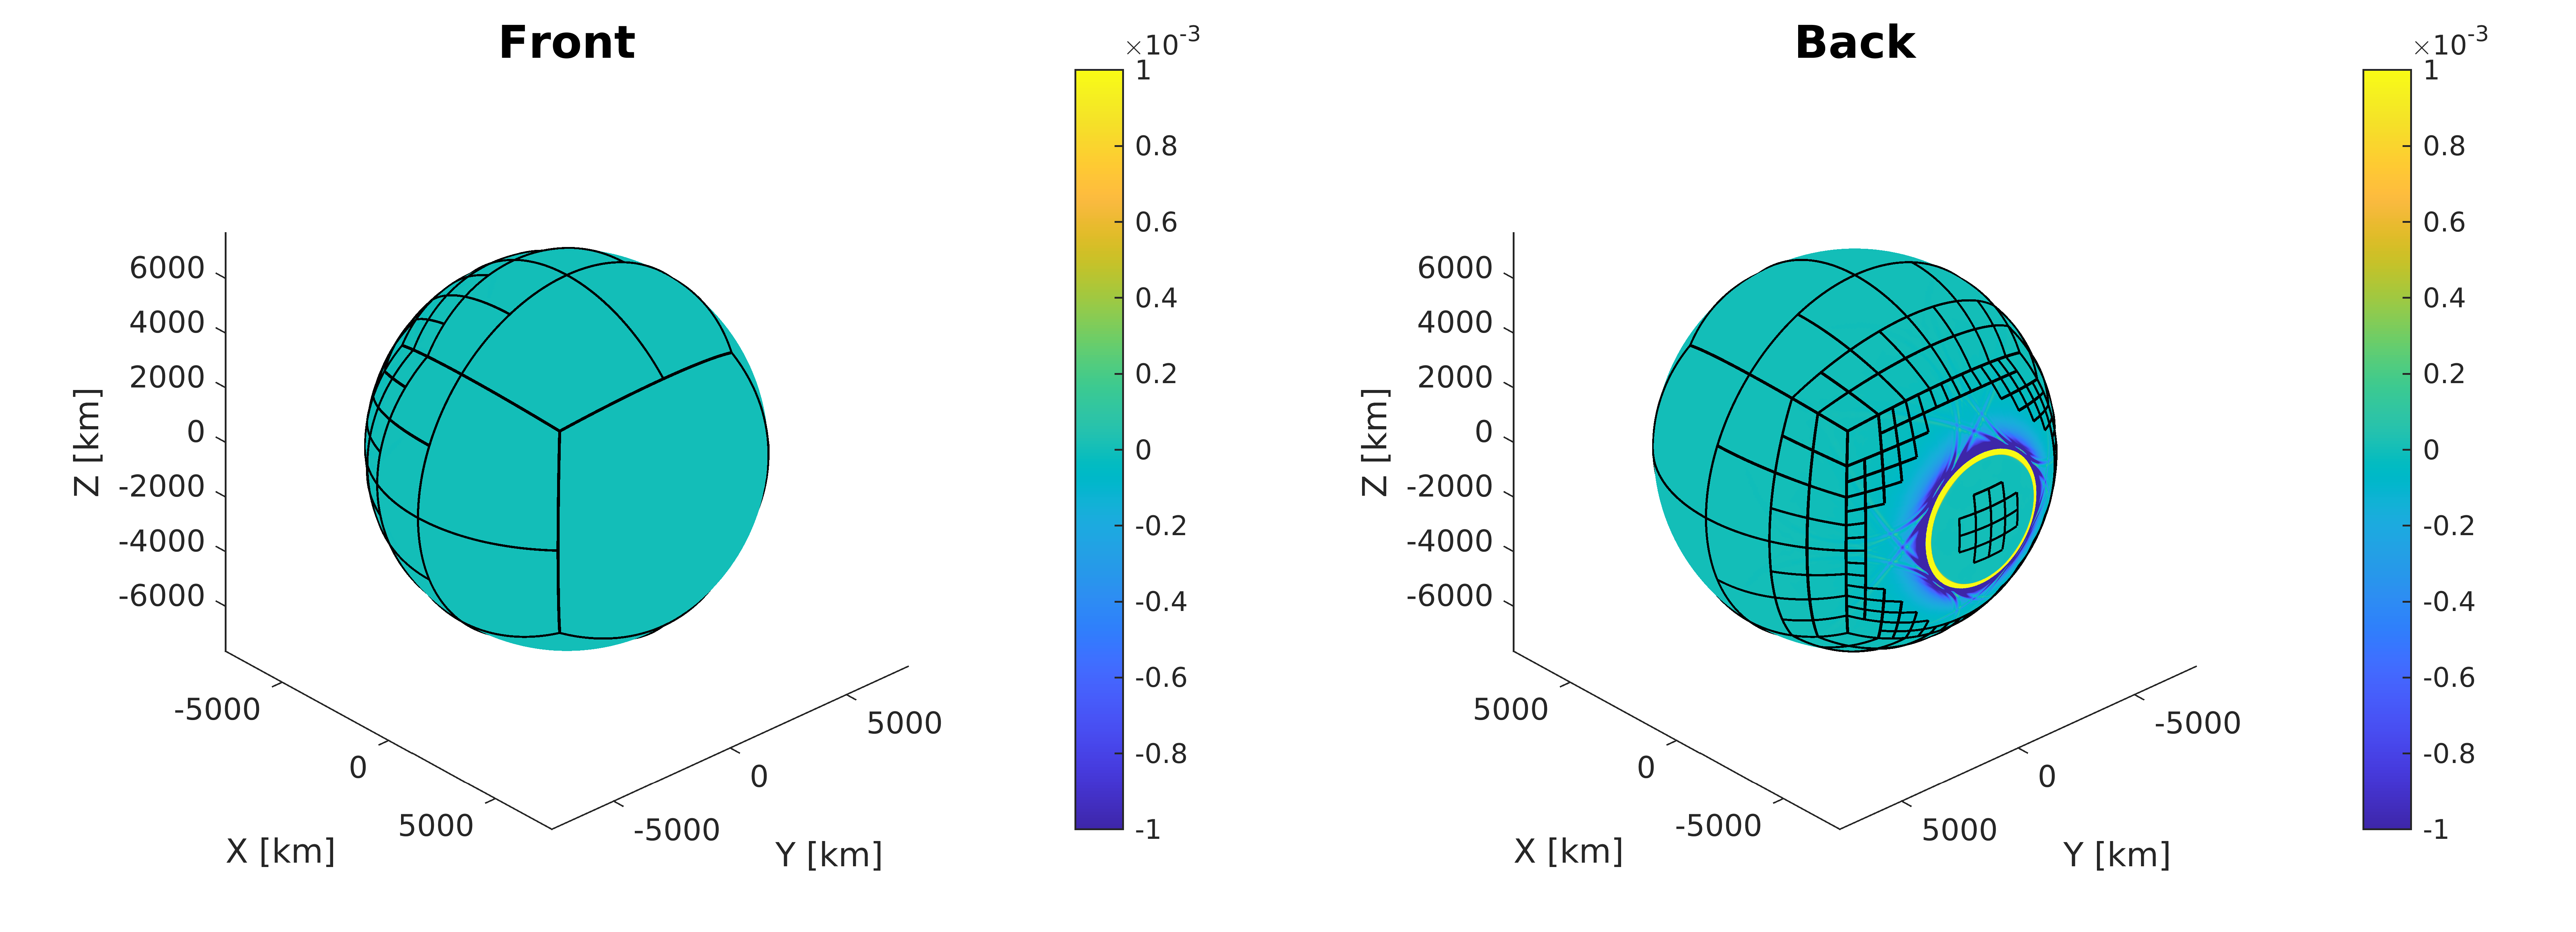
\includegraphics[width=0.95\textwidth,clip=True,trim=4cm 0cm 4cm 0cm]{images/ideal/ideal_24.png}
  \caption{Time: 12 hours }
\end{subfigure}

\caption{Solution: 15 January 2022, 04:00 $\mathrm{UTC}$ - 16 January 2022, 04:00 $\mathrm{UTC}$}
\end{figure}

\medskip

\begin{figure}[!htbp]\ContinuedFloat
\vspace{-15pt}
\centering

\begin{subfigure}{\textwidth}
  \centering
  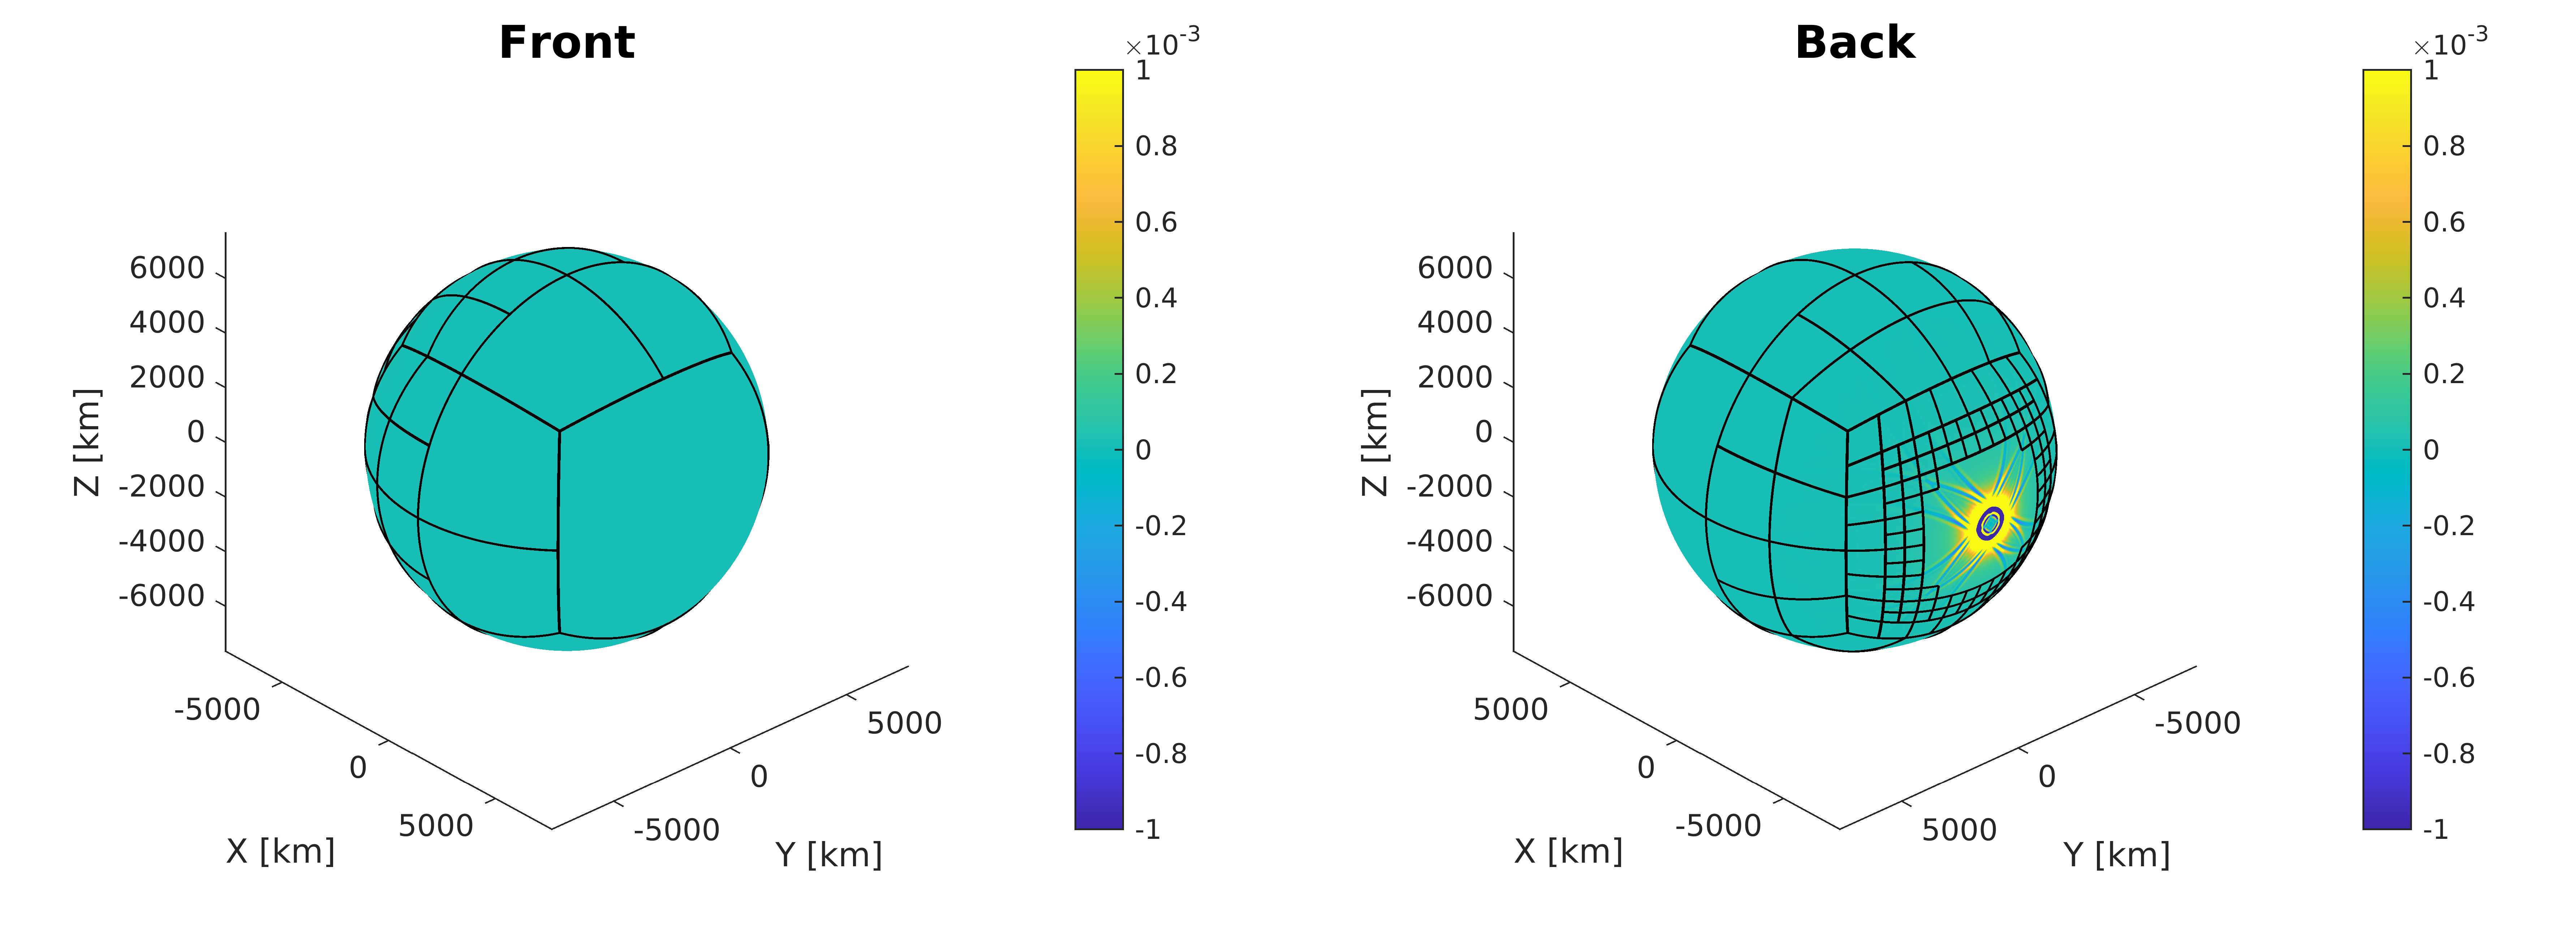
\includegraphics[width=0.95\textwidth,clip=True,trim=4cm 0cm 4cm 0cm]{images/ideal/ideal_28.png}
  \caption{Time: 14 hours }
\end{subfigure}

\medskip

\begin{subfigure}{\textwidth}
  \centering
  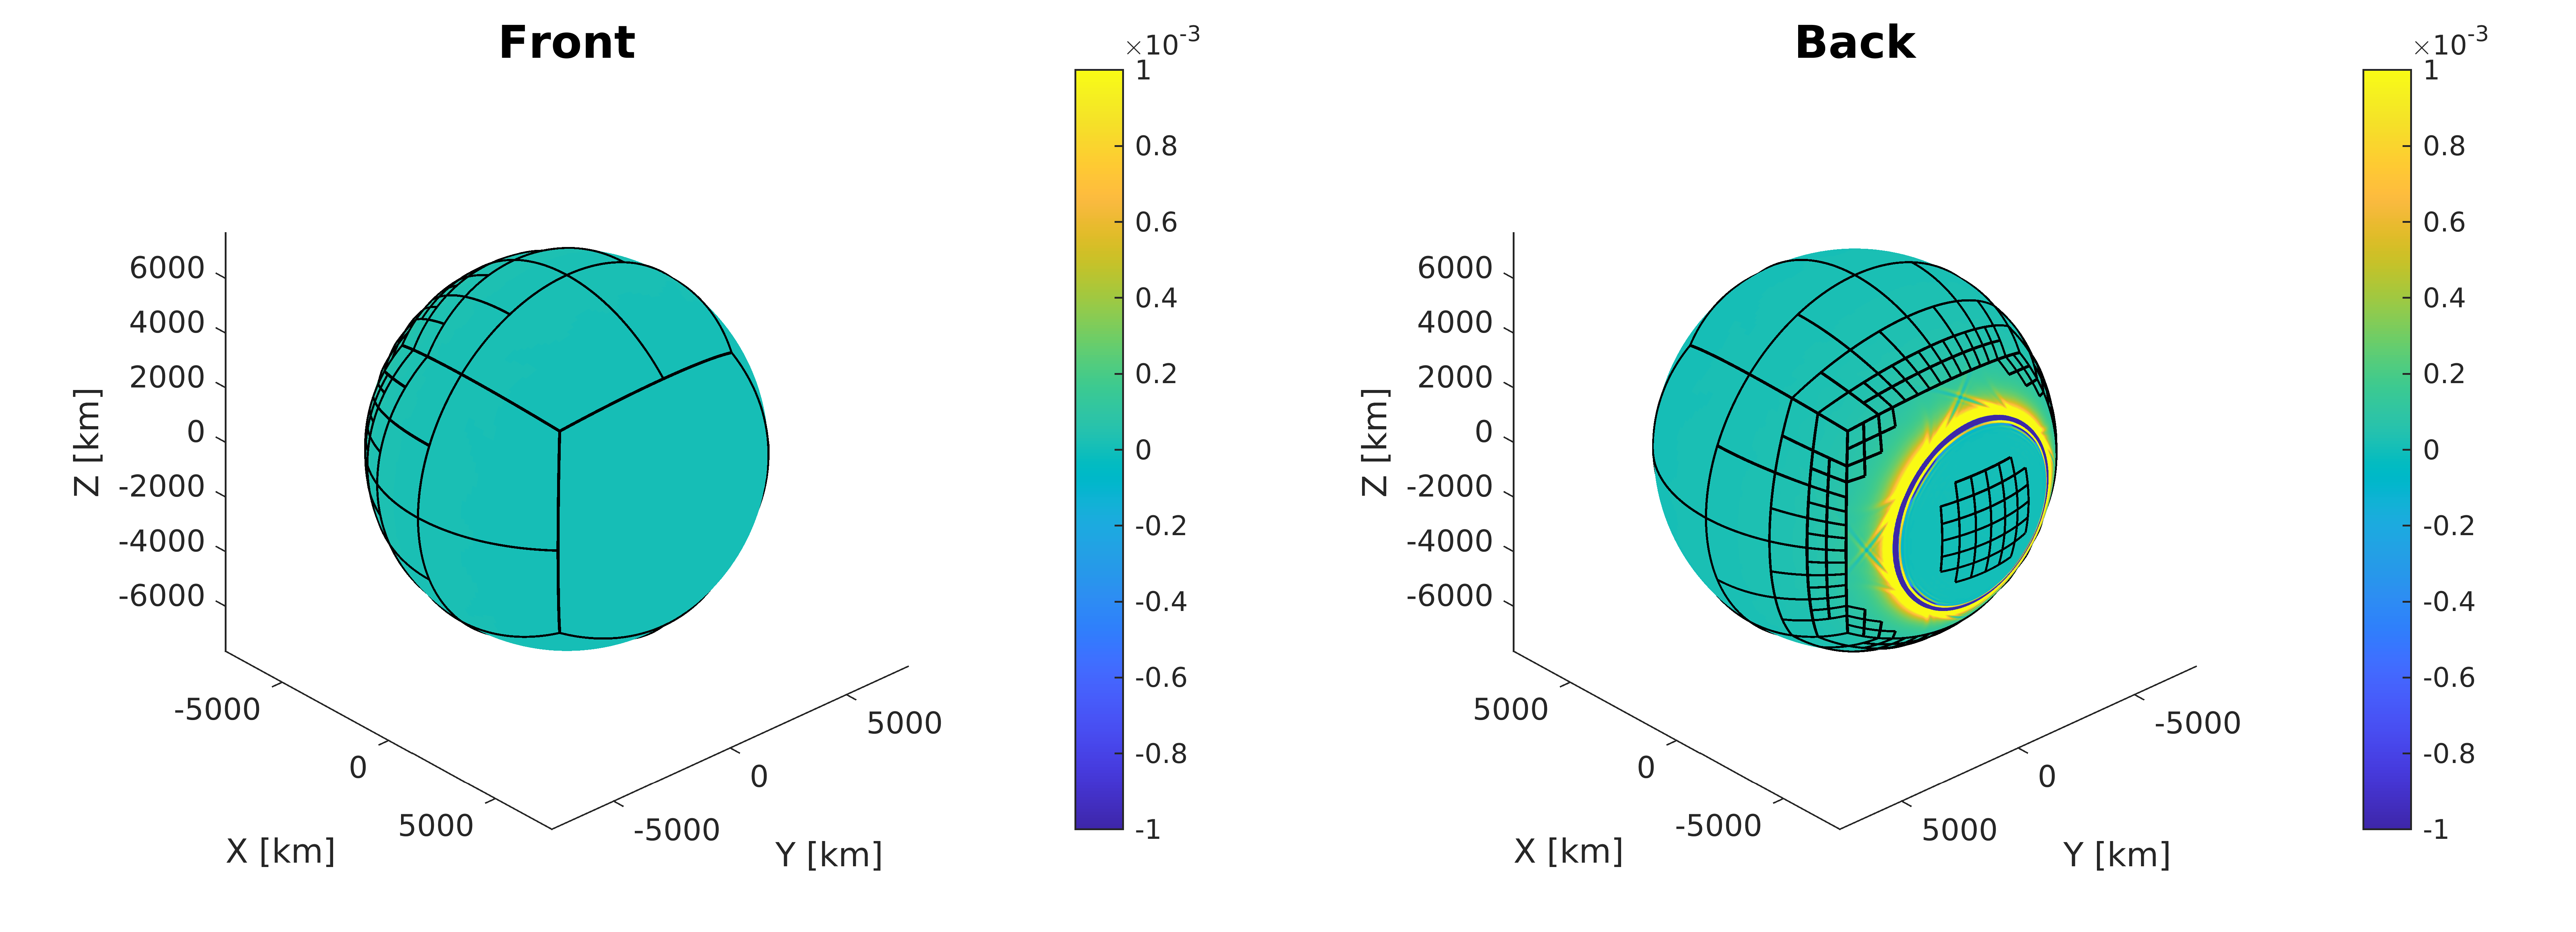
\includegraphics[width=0.95\textwidth,clip=True,trim=4cm 0cm 4cm 0cm]{images/ideal/ideal_32.png}
  \caption{Time: 16 hours }
\end{subfigure}

\medskip

\begin{subfigure}{\textwidth}
  \centering
  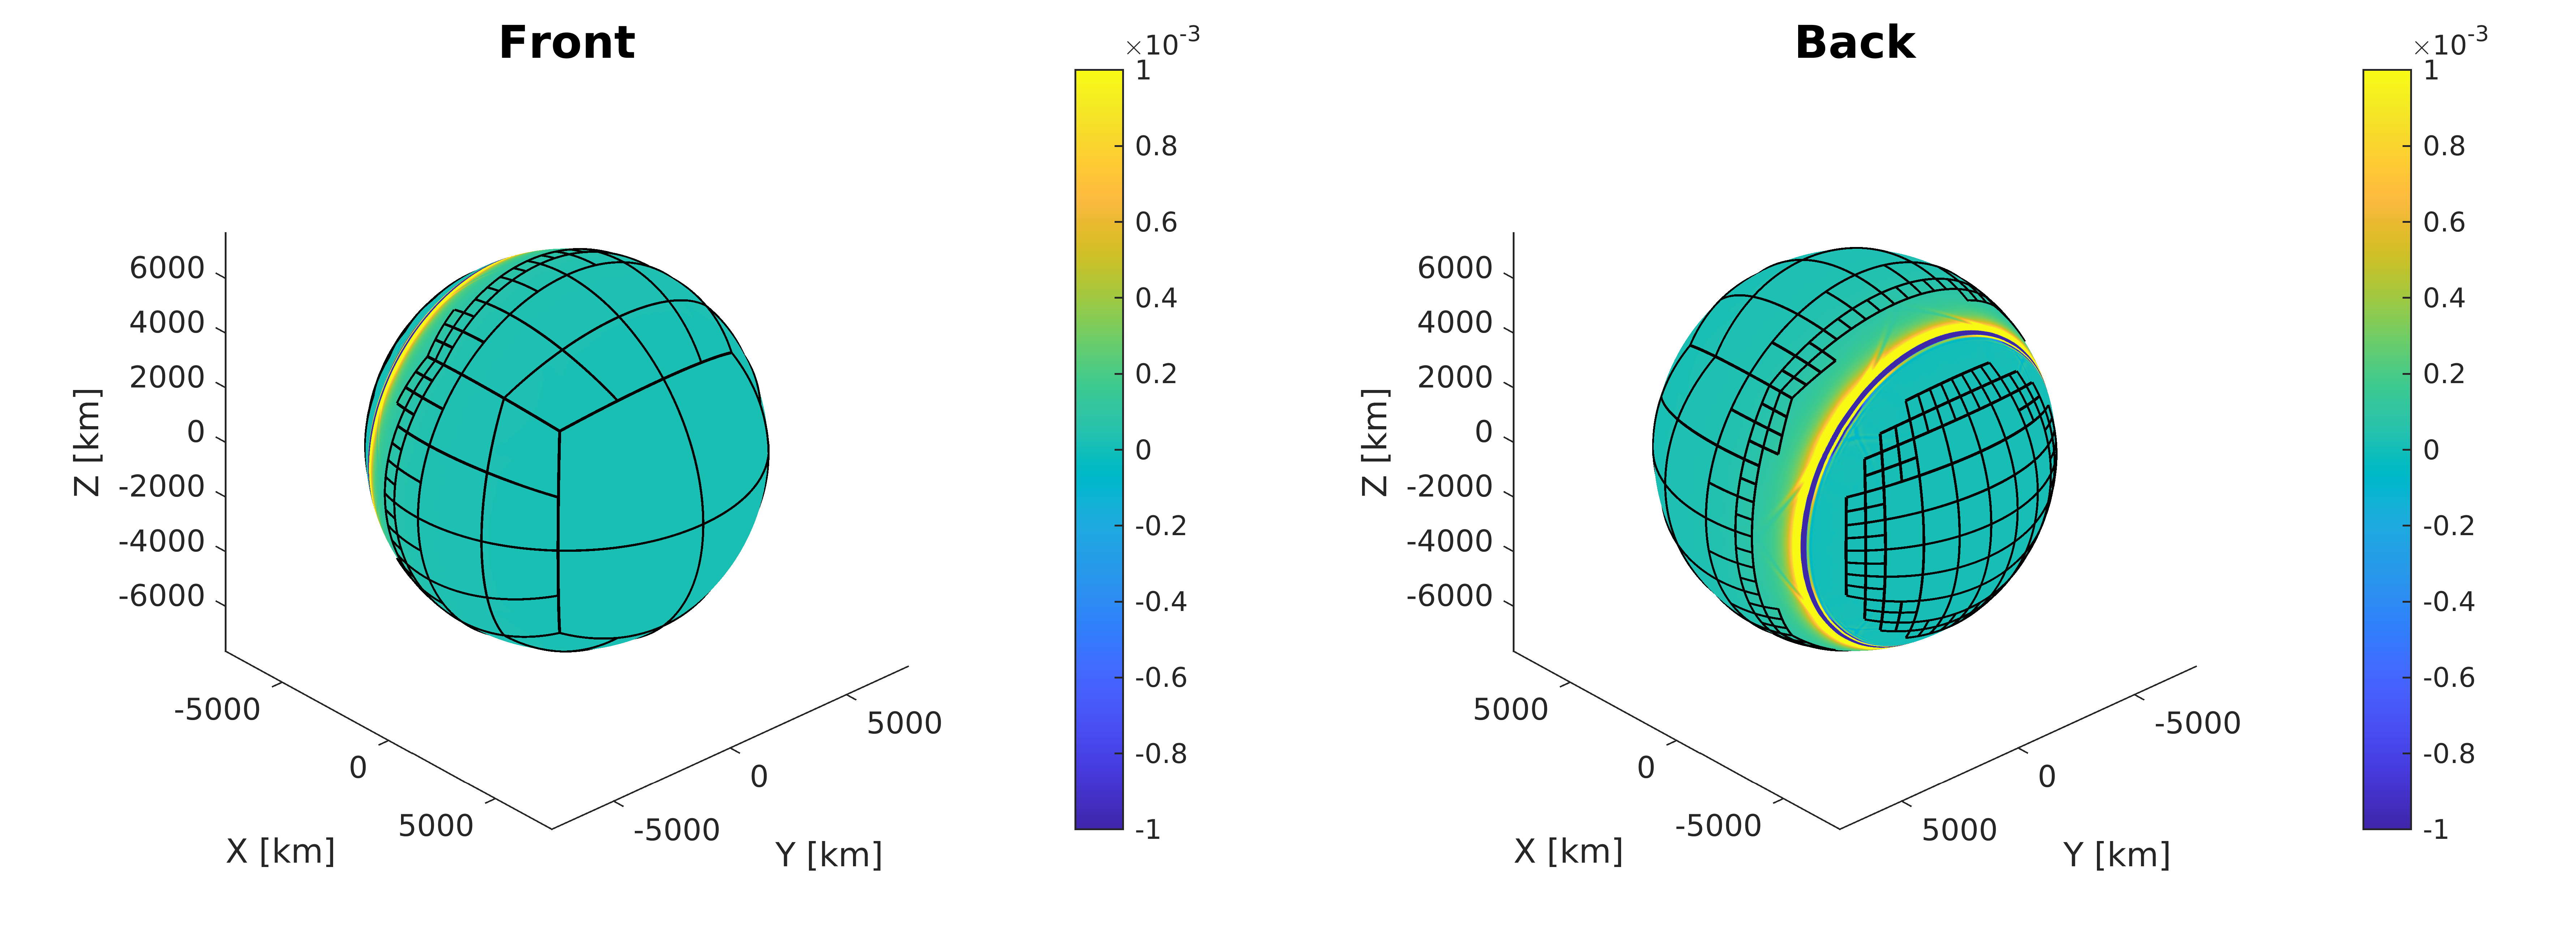
\includegraphics[width=0.95\textwidth,clip=True,trim=4cm 0cm 4cm 0cm]{images/ideal/ideal_36.png}
  \caption{Time: 18 hours }
\end{subfigure}

\caption{Solution: 15 January 2022, 04:00 $\mathrm{UTC}$ - 16 January 2022, 04:00 $\mathrm{UTC}$}
\end{figure}

\medskip

\begin{figure}[!htbp]\ContinuedFloat
\vspace{-15pt}
\centering
\begin{subfigure}{\textwidth}
  \centering
  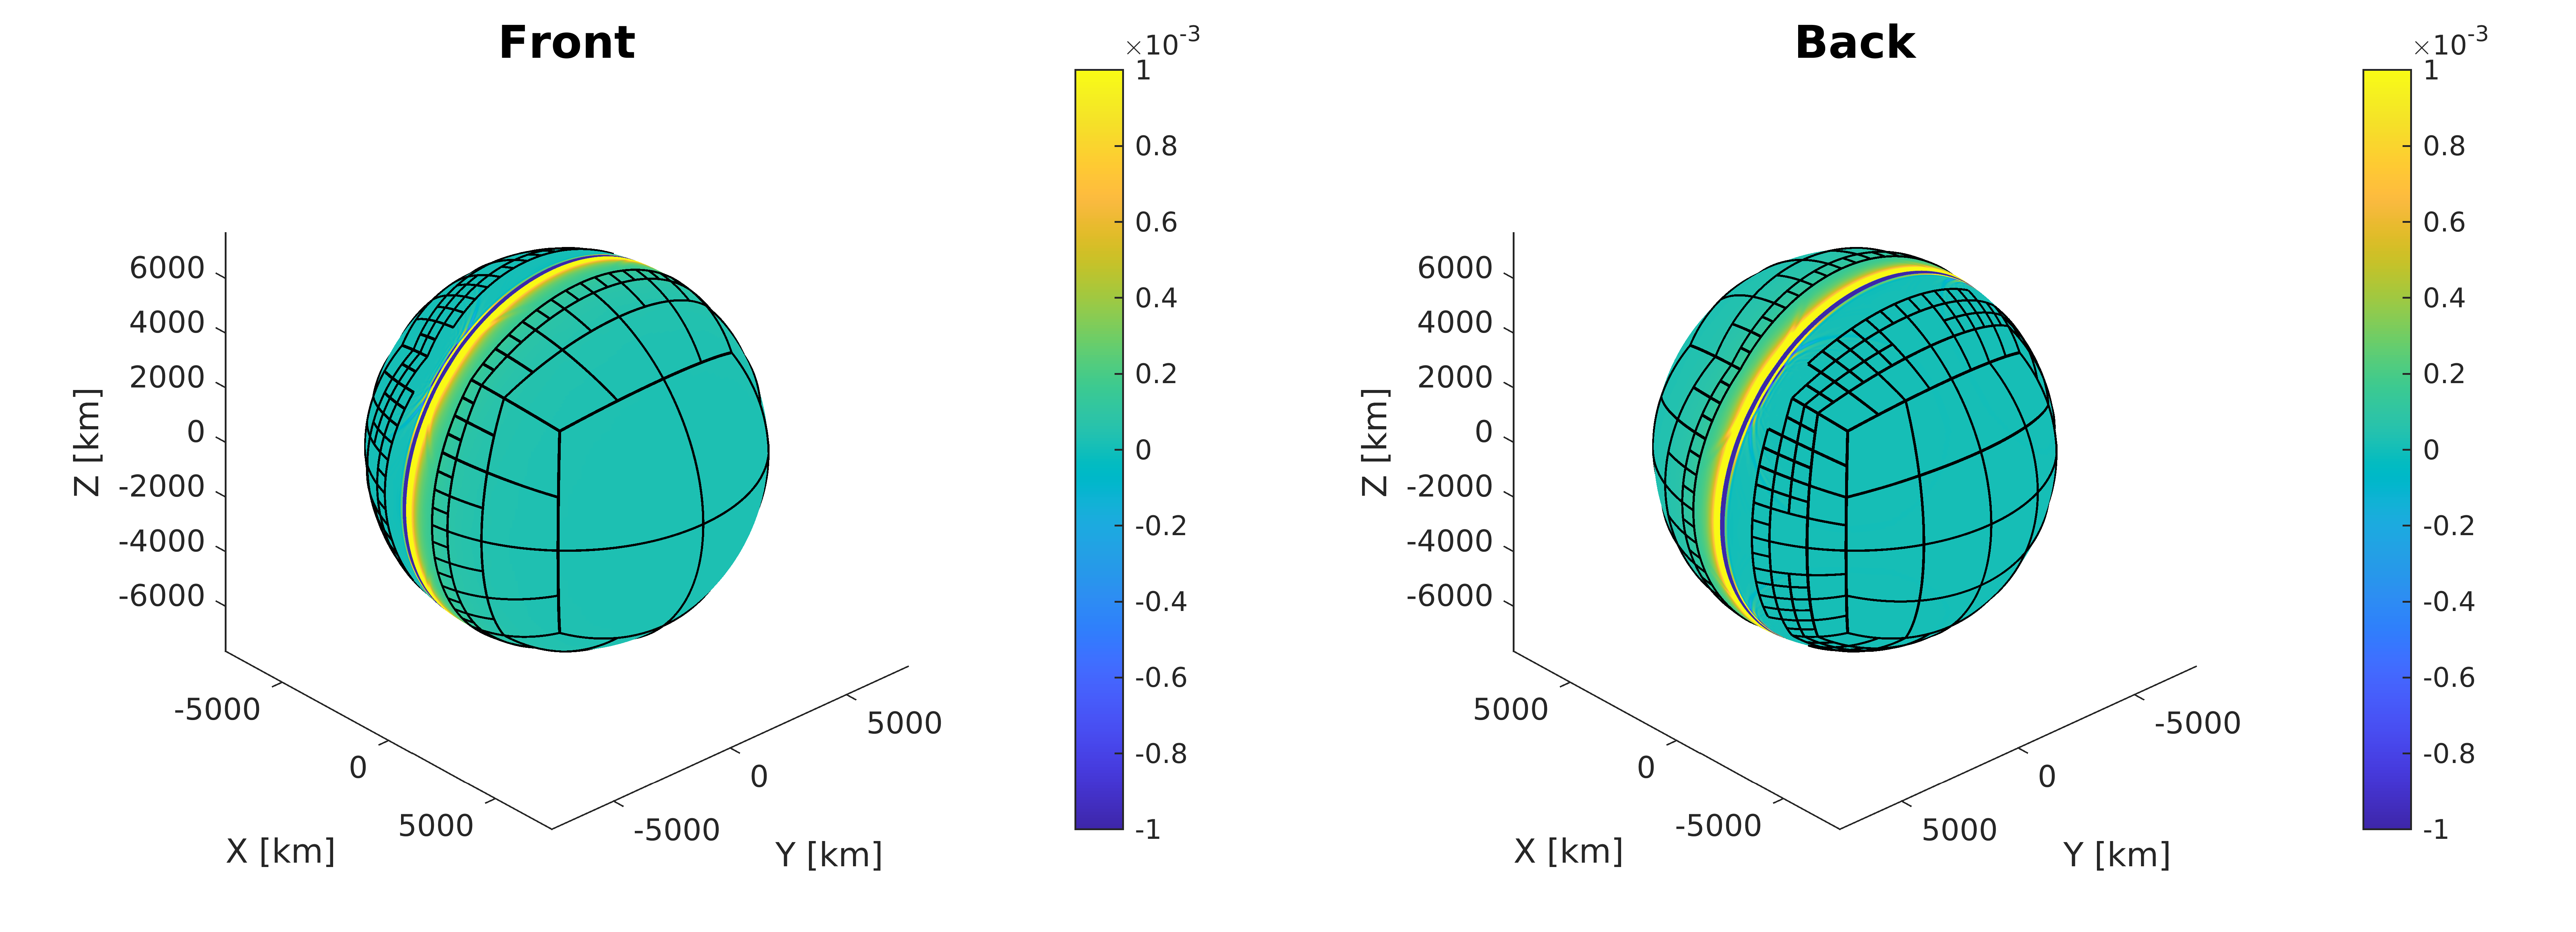
\includegraphics[width=0.95\textwidth,clip=True,trim=4cm 0cm 4cm 0cm]{images/ideal/ideal_40.png}
  \caption{Time: 20 hours }
\end{subfigure}

\medskip

\begin{subfigure}{\textwidth}
  \centering
  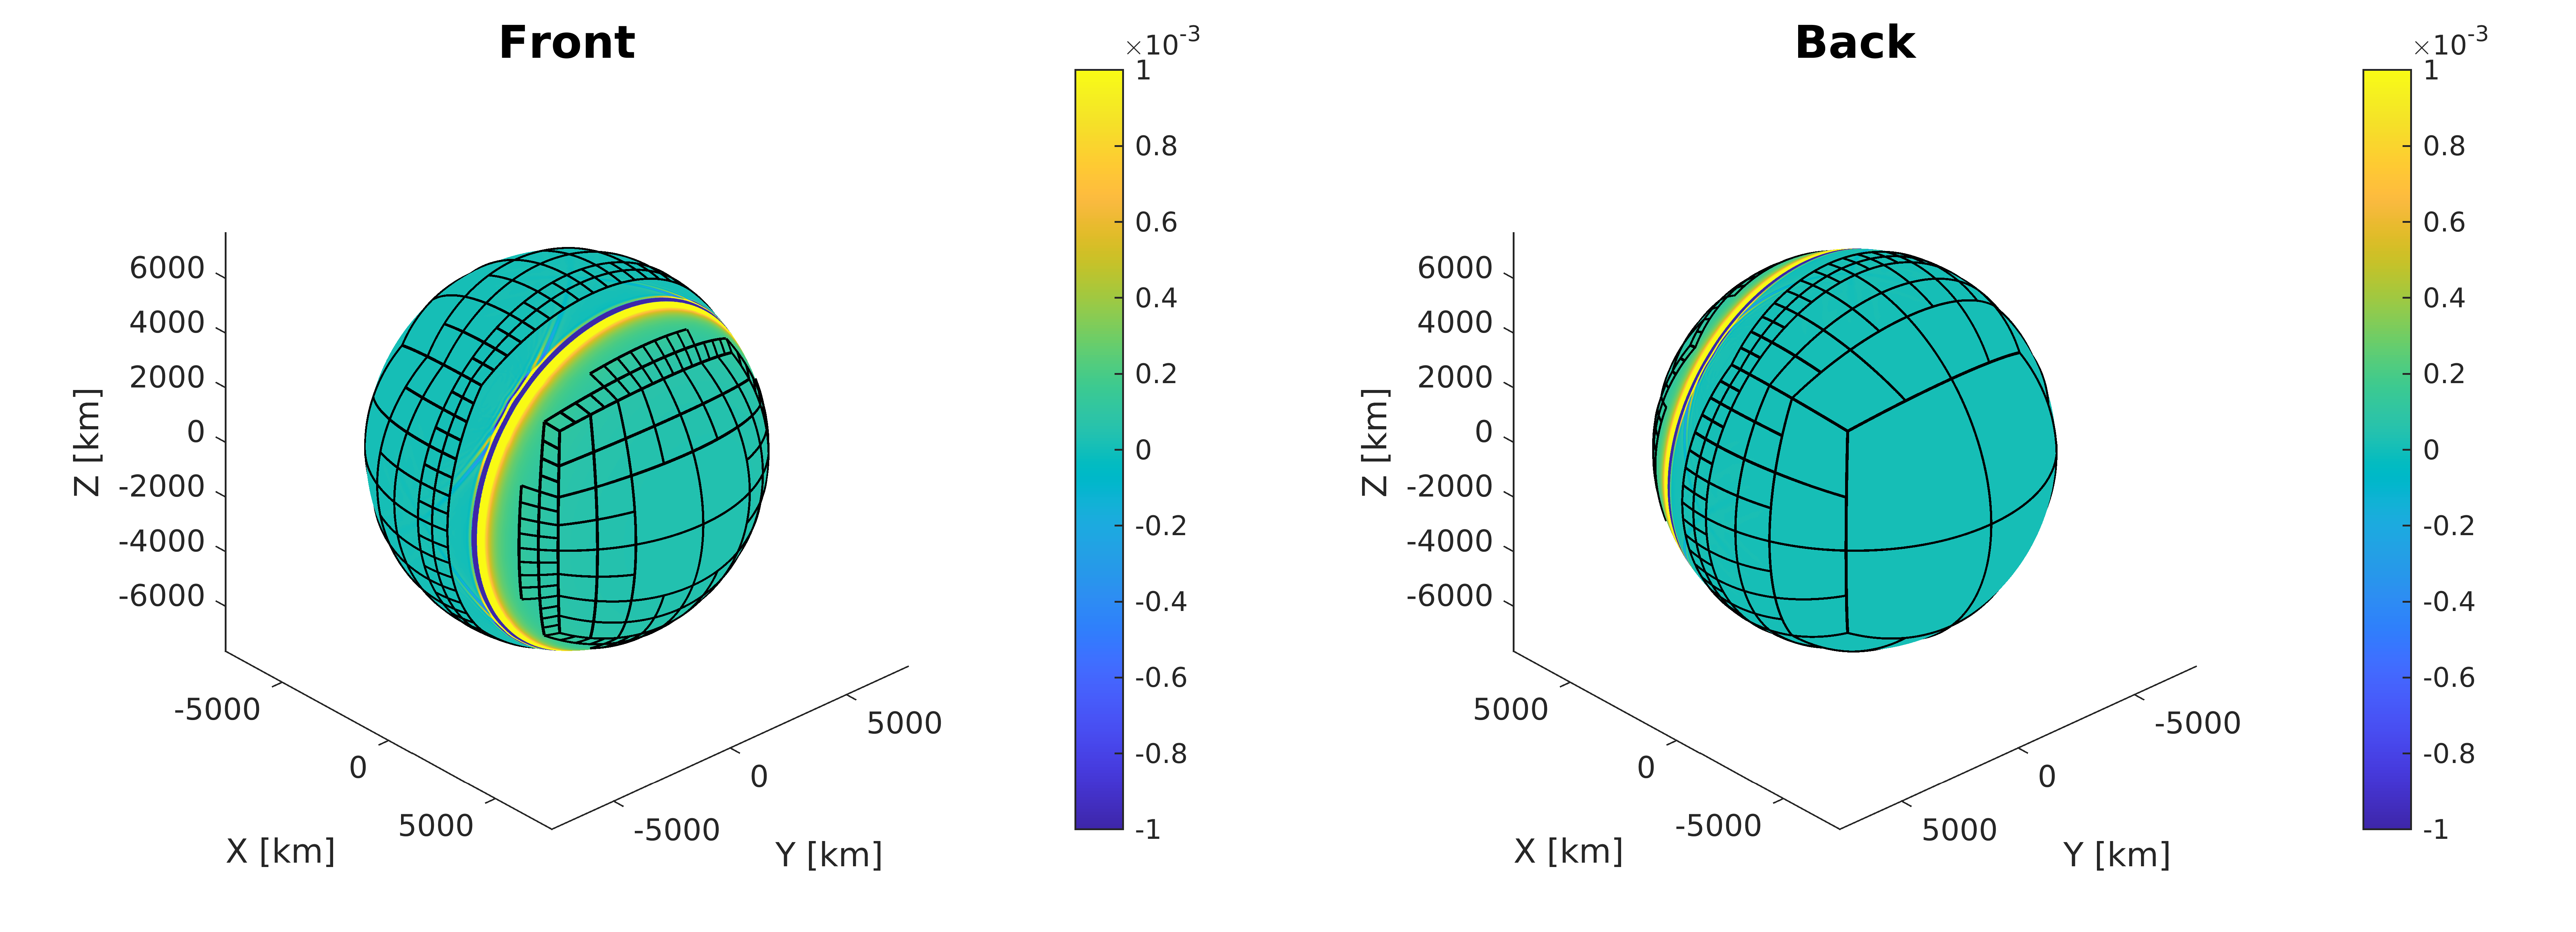
\includegraphics[width=0.95\textwidth,clip=True,trim=4cm 0cm 4cm 0cm]{images/ideal/ideal_44.png}
  \caption{Time: 22 hours}
  \end{subfigure}

\medskip

\begin{subfigure}{\textwidth}
  \centering
  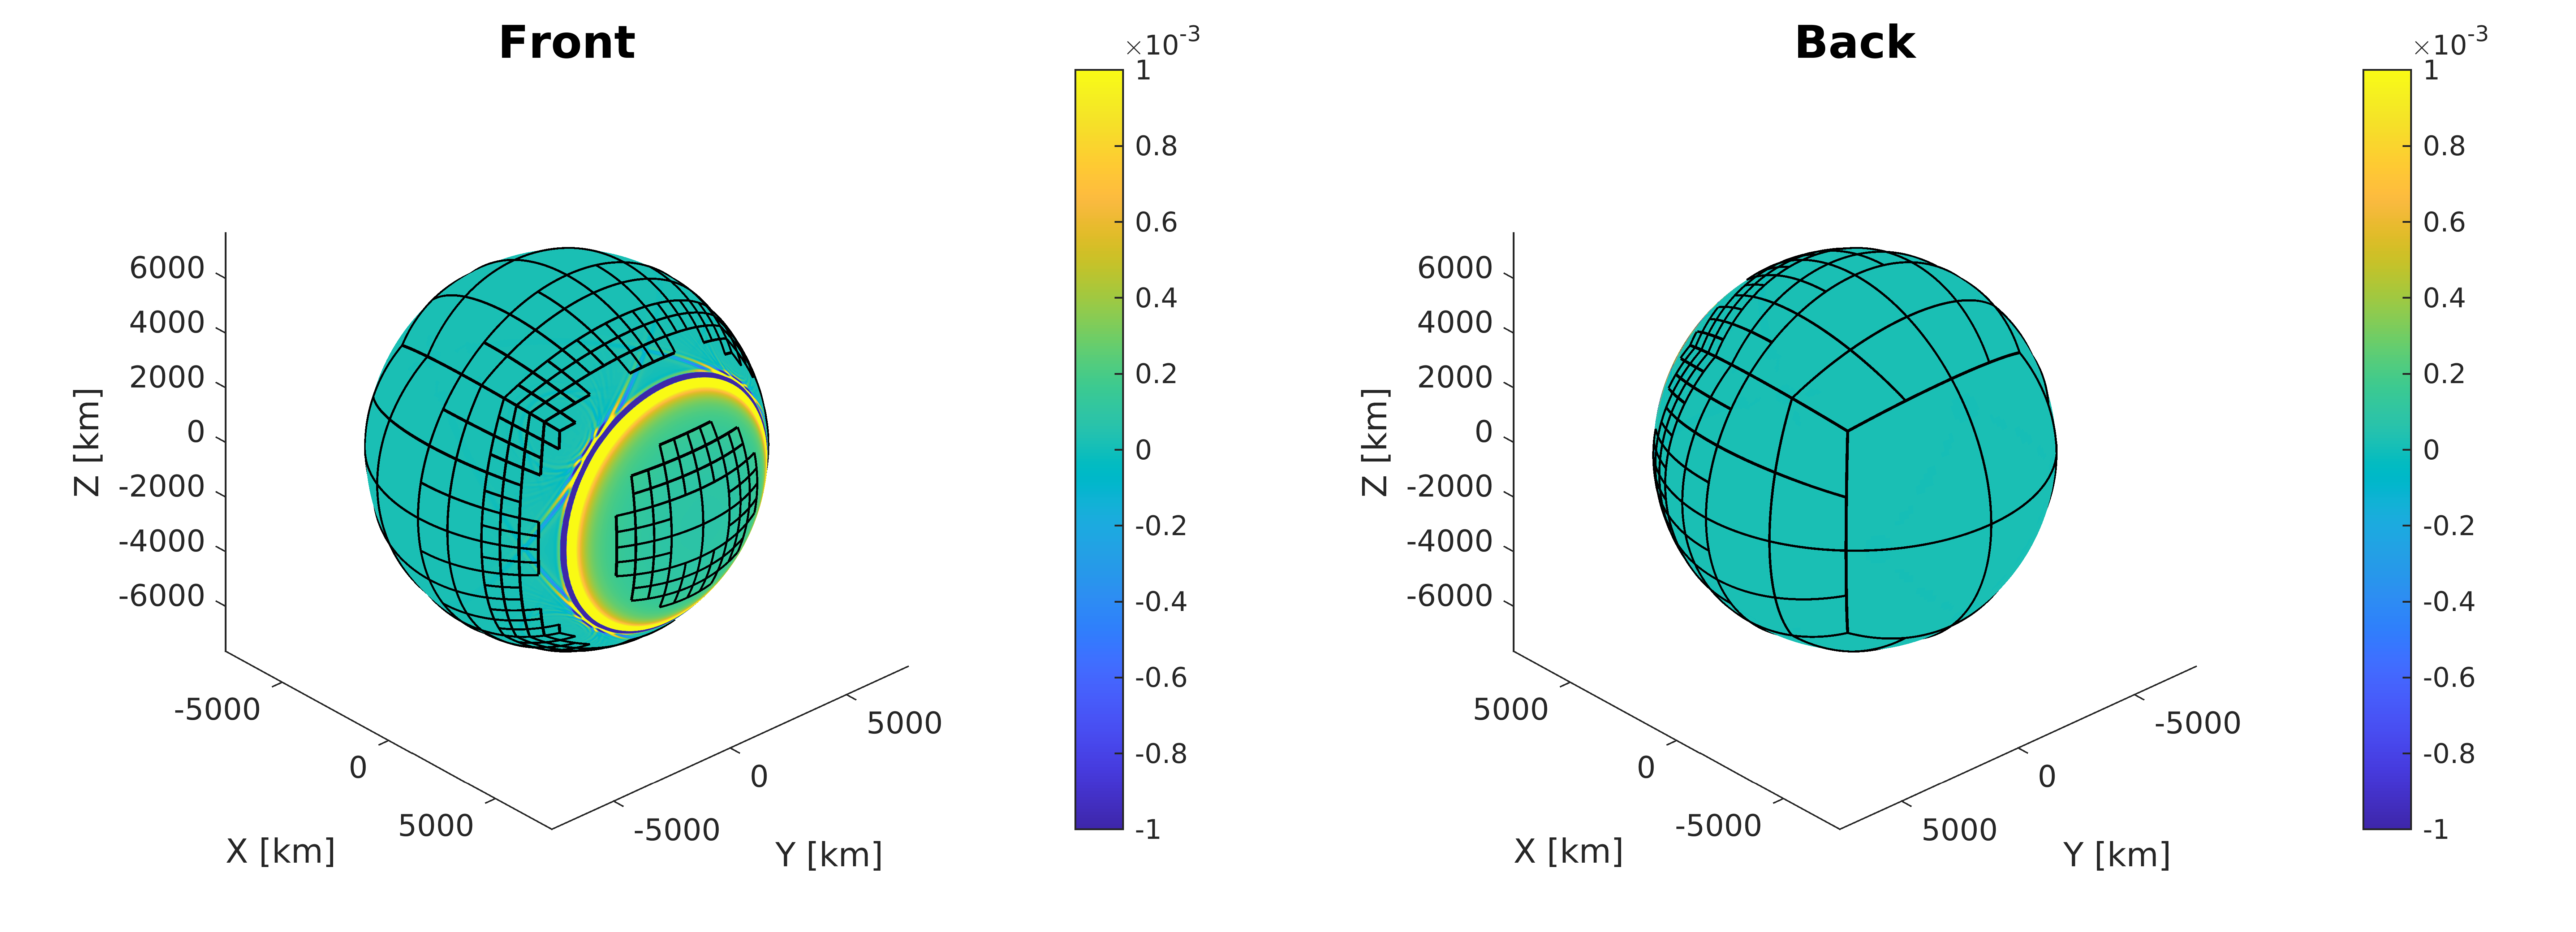
\includegraphics[width=0.95\textwidth,clip=True,trim=4cm 0cm 4cm 0cm]{images/ideal/ideal_48.png}
  \caption{Time: 24 hours }
\end{subfigure}

\caption{Solution: 15 January 2022, 04:00 $\mathrm{UTC}$ - 16 January 2022, 04:00 $\mathrm{UTC}$}
\label{fig:3.2}
\end{figure}
We observed that the wave travels halfway around the cubed sphere $R=6378100$ $\mathrm{m}$ in a time period of 6.5 - 7 hours. Figure \ref{fig:3.3} shows the scatter plot of wave height verses angle with axis of spherical symmetry (e.g. $(x,y,z)=(1,0,0)$). Note that the scatter plots presented here use refinement up to level 6.
\begin{figure}[!htbp]
    \centering
    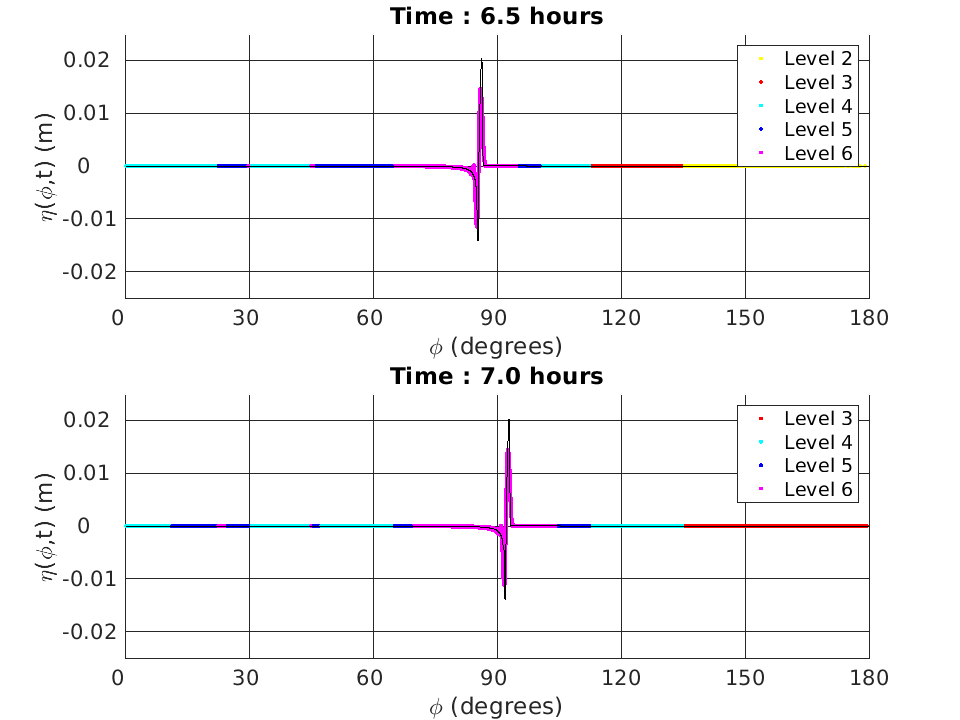
\includegraphics[width=\textwidth]{images/main1d.png}
    \caption{Scatter plot of wave arrival at the half way point, using an average height field of 17 $\mathrm[km]$.}
    \label{fig:3.3}
\end{figure}
Figure \ref{fig:3.4} shows the waves position for every half-hour time step.
\begin{figure}[!htbp]
    \centering
    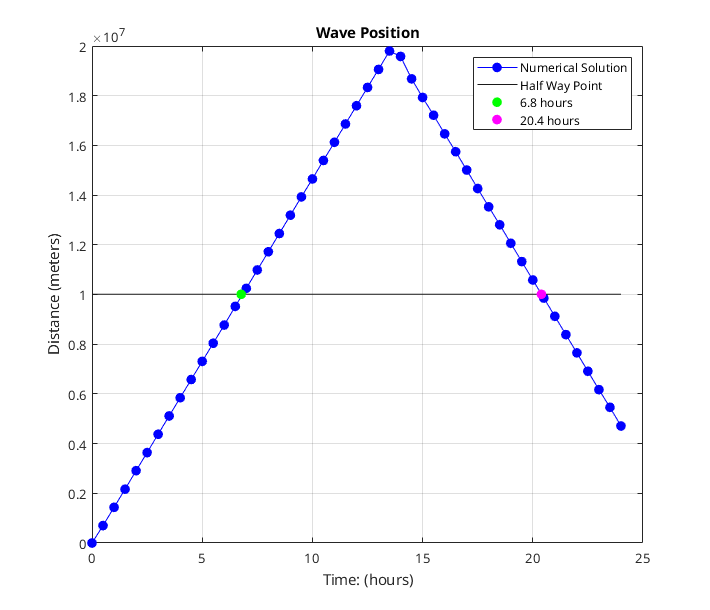
\includegraphics[width=\textwidth]{images/wavepos.png}
    \caption{Plot of distance versus time of traveling Lamb wave.}
    \label{fig:3.4}
\end{figure}
Figure \ref{fig:3.5} shows the waves velocity for each half-hour time step and compares it to characteristic wave speed $c=\sqrt{gH}$ where $H=17$ $\mathrm{km}$ in this case.
\begin{figure}[!htbp]
    \centering
    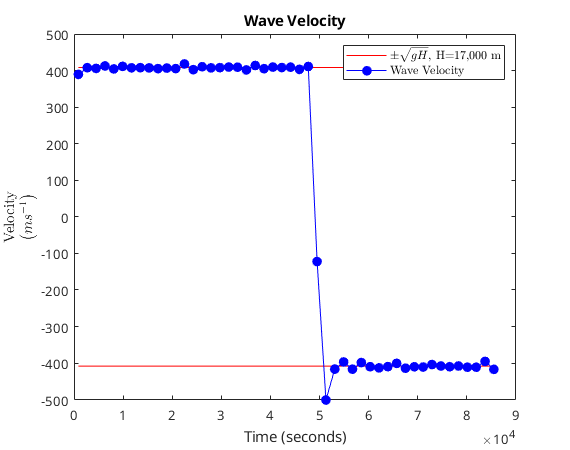
\includegraphics[width=\textwidth]{images/wavevelocity.png}
    \caption{Plot of the wave velocity versus time. Also shown is characteristic speed $\sqrt{g H}$. }
    \label{fig:3.5}
\end{figure}
From this we calculate the wave velocity to be $\sim403.8$ $\mathrm{ms}^{-1}$. This is much faster than the theoretical speed of Lamb wave which is $312$ $\mathrm{ms}^{-1}$ \cite{bretherton1969lamb}. This wave also moves much faster than the model produced by Amores et al. \cite{amores2022numerical} which more closely matched the sensor data and the theoretical speed of Lamb waves. This is due to the extreme heights of the waves which occurred by excluding any kind of bathymetry.
%%%%%%%%%%%%%%%%%%%%%%%%%%%%%%%%%%%%%%%%%%%%%%%%%%%%%%%%%%%%%%%%%%%%%%%%%%%%%%
%
% Chapter: Incorporating Temperature as Bathymetry
%
%%%%%%%%%%%%%%%%%%%%%%%%%%%%%%%%%%%%%%%%%%%%%%%%%%%%%%%%%%%%%%%%%%%%%%%%%%%%%%
\chapter{Incorporating Temperature as Bathymetry}\label{ch:4}
Having verified that we can get reasonable results that match theoretical expectations for a given wave height, we can use this type of model in an attempt to solve a more complicated problem in a similar way. The speed of our wave in the Section \ref{sec:3.2} traveled slightly faster than the theoretical speed of Lamb waves. In the homogeneous model there was no accounting for variations in air temperature which would effect the velocity of the waves. To model these variations in air temperature we can assume that the tropopause is at a constant temperature, and that the temperature below in troposphere acts as a type of bathymetry.
\begin{figure}[!htbp]
	\centering
	\includestandalone[width=\textwidth]{IC_temp}
	\caption{Initial Conditions and the Shallow Water Model With Temperature as Bathymetry}
	\label{fig:4.1}
\end{figure}
 We can use the relationship between speed of sound and temperature to calculate the bathymetry terms as proposed by Amores et al. \cite{amores2022numerical} and discussed in Section \ref{sec:1.2}. Recall from Section \ref{subsec:1.1.3} that the velocity of a wave from the shallow water equations is 
 \begin{equation}\label{eq:4.1}
    c =\sqrt{gH}.
 \end{equation}
 Also recall that Lamb waves are somewhat similar to acoustic waves in that they travel close to the speed of sound. The velocity of a sound wave dependent on temperature is given by
 \begin{equation}\label{eq:4.2}
     c=\sqrt{\frac{\gamma R T}{M}}.
 \end{equation}
 Equating the two wave velocities
\begin{equation}\label{eq:4.3}
	\sqrt{gH}=\sqrt{\frac{\gamma R T}{M}}
\end{equation}
and solving for $H$ results in 
\begin{equation}\label{eq:4.4}
	H=\frac{\gamma R T}{Mg}.
\end{equation}
This is the height at which the shallow water model would need to be scaled for that given temperature.\\
\indent Using the same ERA5 reanalysis temperature data as Amores et al. \cite{amores2022numerical} we can take the vertical average between the reading at 2 $\mathrm{m}$ and 100 $\mathrm{hPa}$. Figure \ref{fig:4.2} below shows a visualization of this at the time of eruption $t=0$.
 \begin{figure}[!htbp]
 \vspace{-15pt}
\centering
\begin{subfigure}{\textwidth}
  \centering
  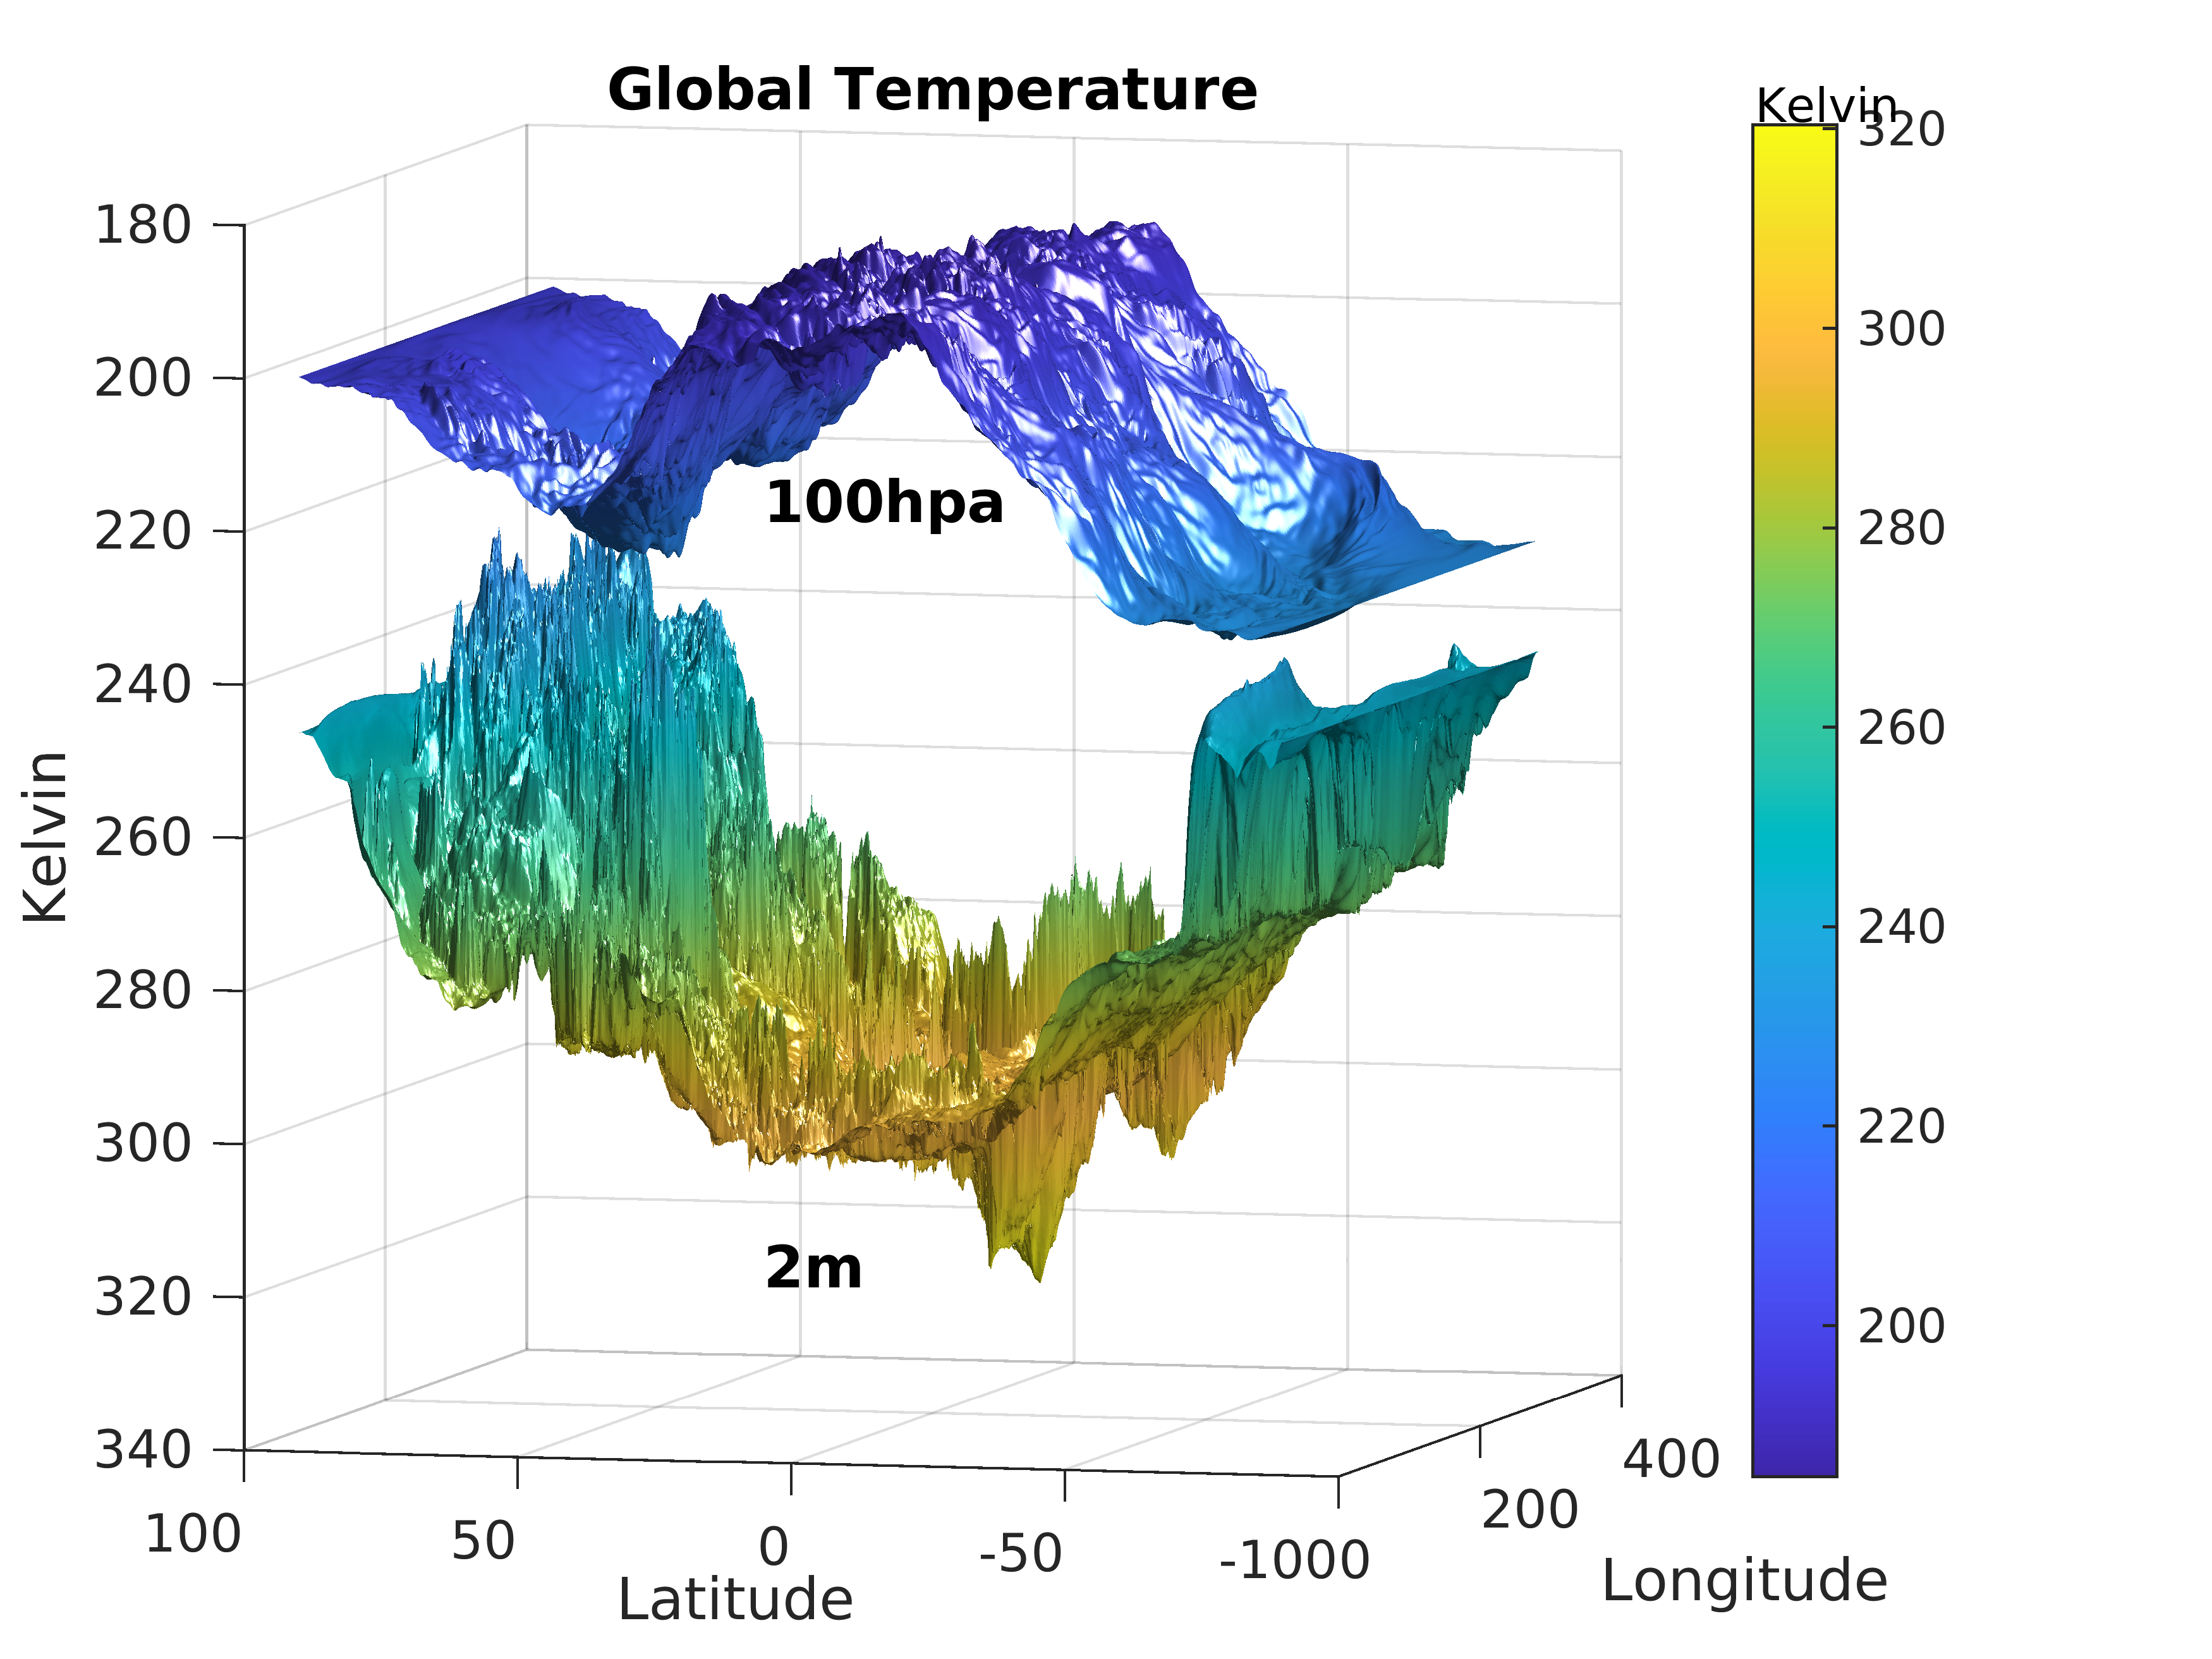
\includegraphics[width=0.7\textwidth,clip=True,trim=0.2cm 0cm 1.7cm 0.3cm]{images/2layer.png}
  \caption{Stacked surface plots of the data layers}
\end{subfigure}%

\medskip

\begin{subfigure}{\textwidth}
  \centering
  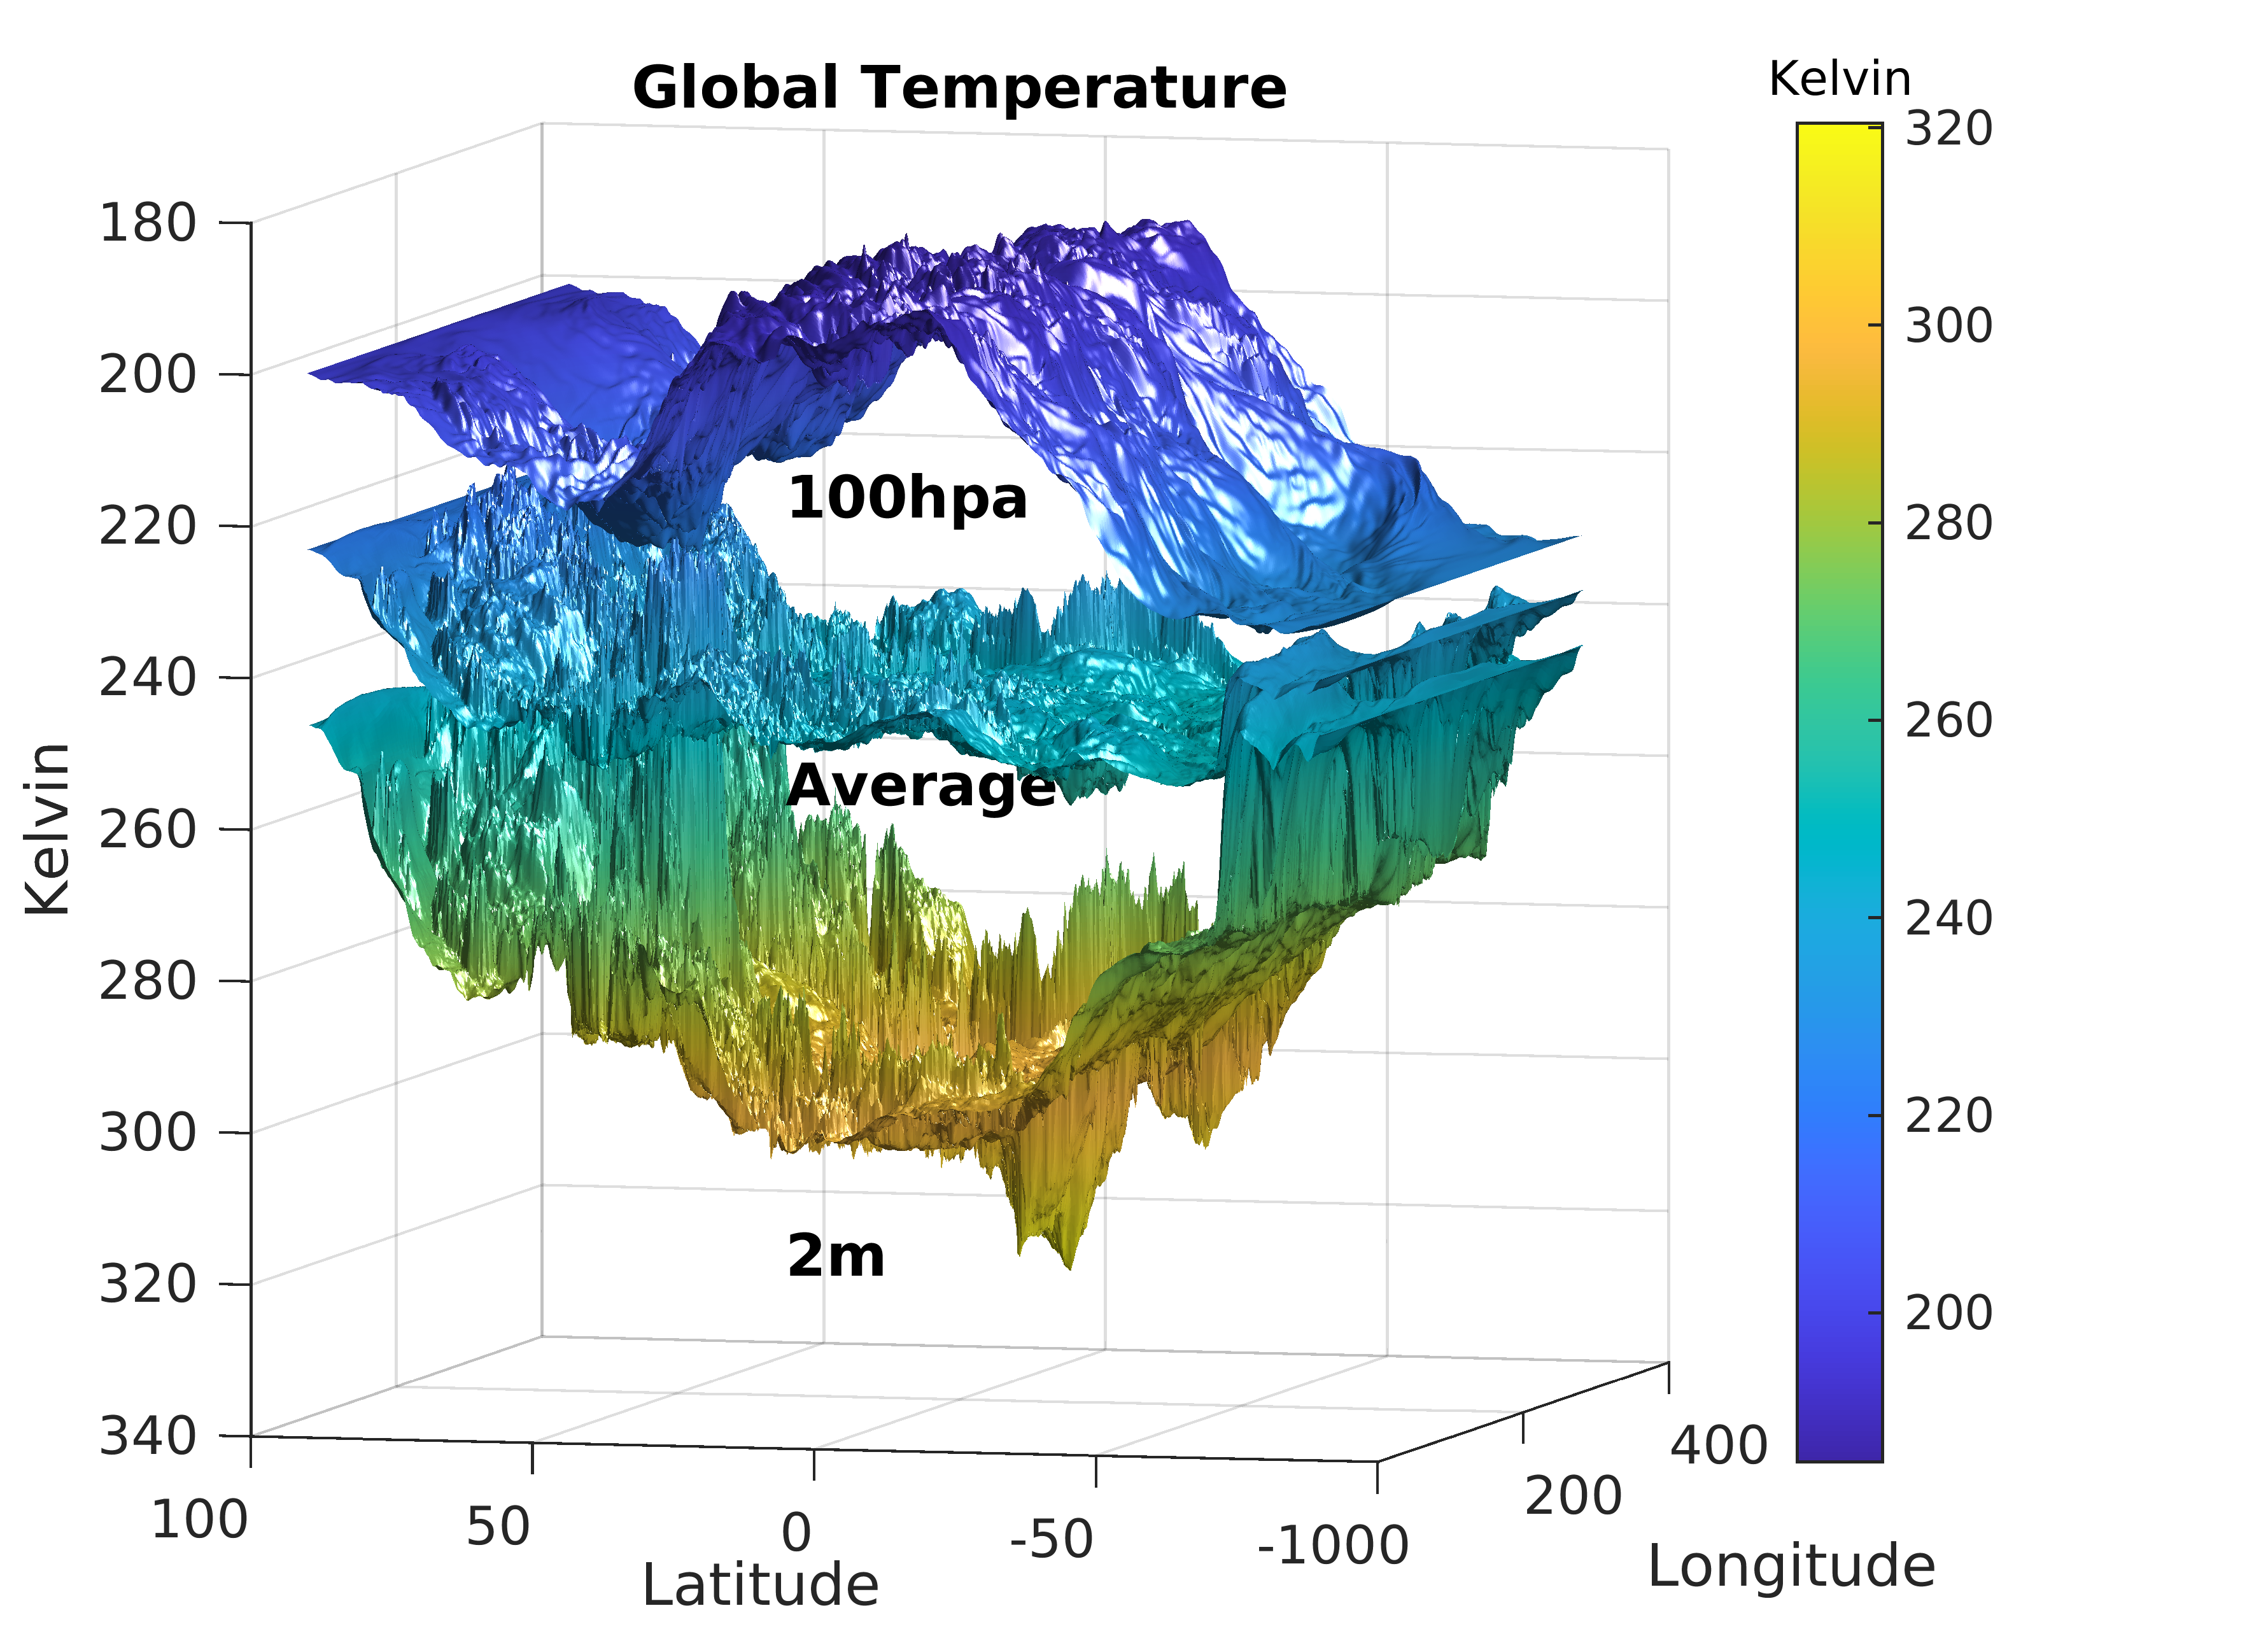
\includegraphics[width=0.7\textwidth,clip=True,trim=0.2cm 0cm 1.7cm 0.3cm]{images/3layer.png}
  \caption{Stacked surface plots of the data layers including the vertical average}
\end{subfigure}
\caption{Global temperature taken 15 January 2022, 04:00 $\mathrm{UTC}$}
\label{fig:4.2}
\end{figure}
For this proposed model we will not consider the bathymetry changes with time. So this vertically averaged temperature can be used to get an average temperature profile over the same five day period, 15 January 2022, 04:00 $\mathrm{UTC}$ through 21 January 2022, 04:00 $\mathrm{UTC}$, as Amores et al. \cite{amores2022numerical} using one hour time steps. Equation \eqref{eq:4.4} then applied to this temperature profile gives the necessary scaling for each water column which is the bathymetry. This idea is demonstrated in figure \ref{fig:4.3}.
 \begin{figure}[!htbp]
\centering
\begin{subfigure}{0.5\textwidth}
  \centering
  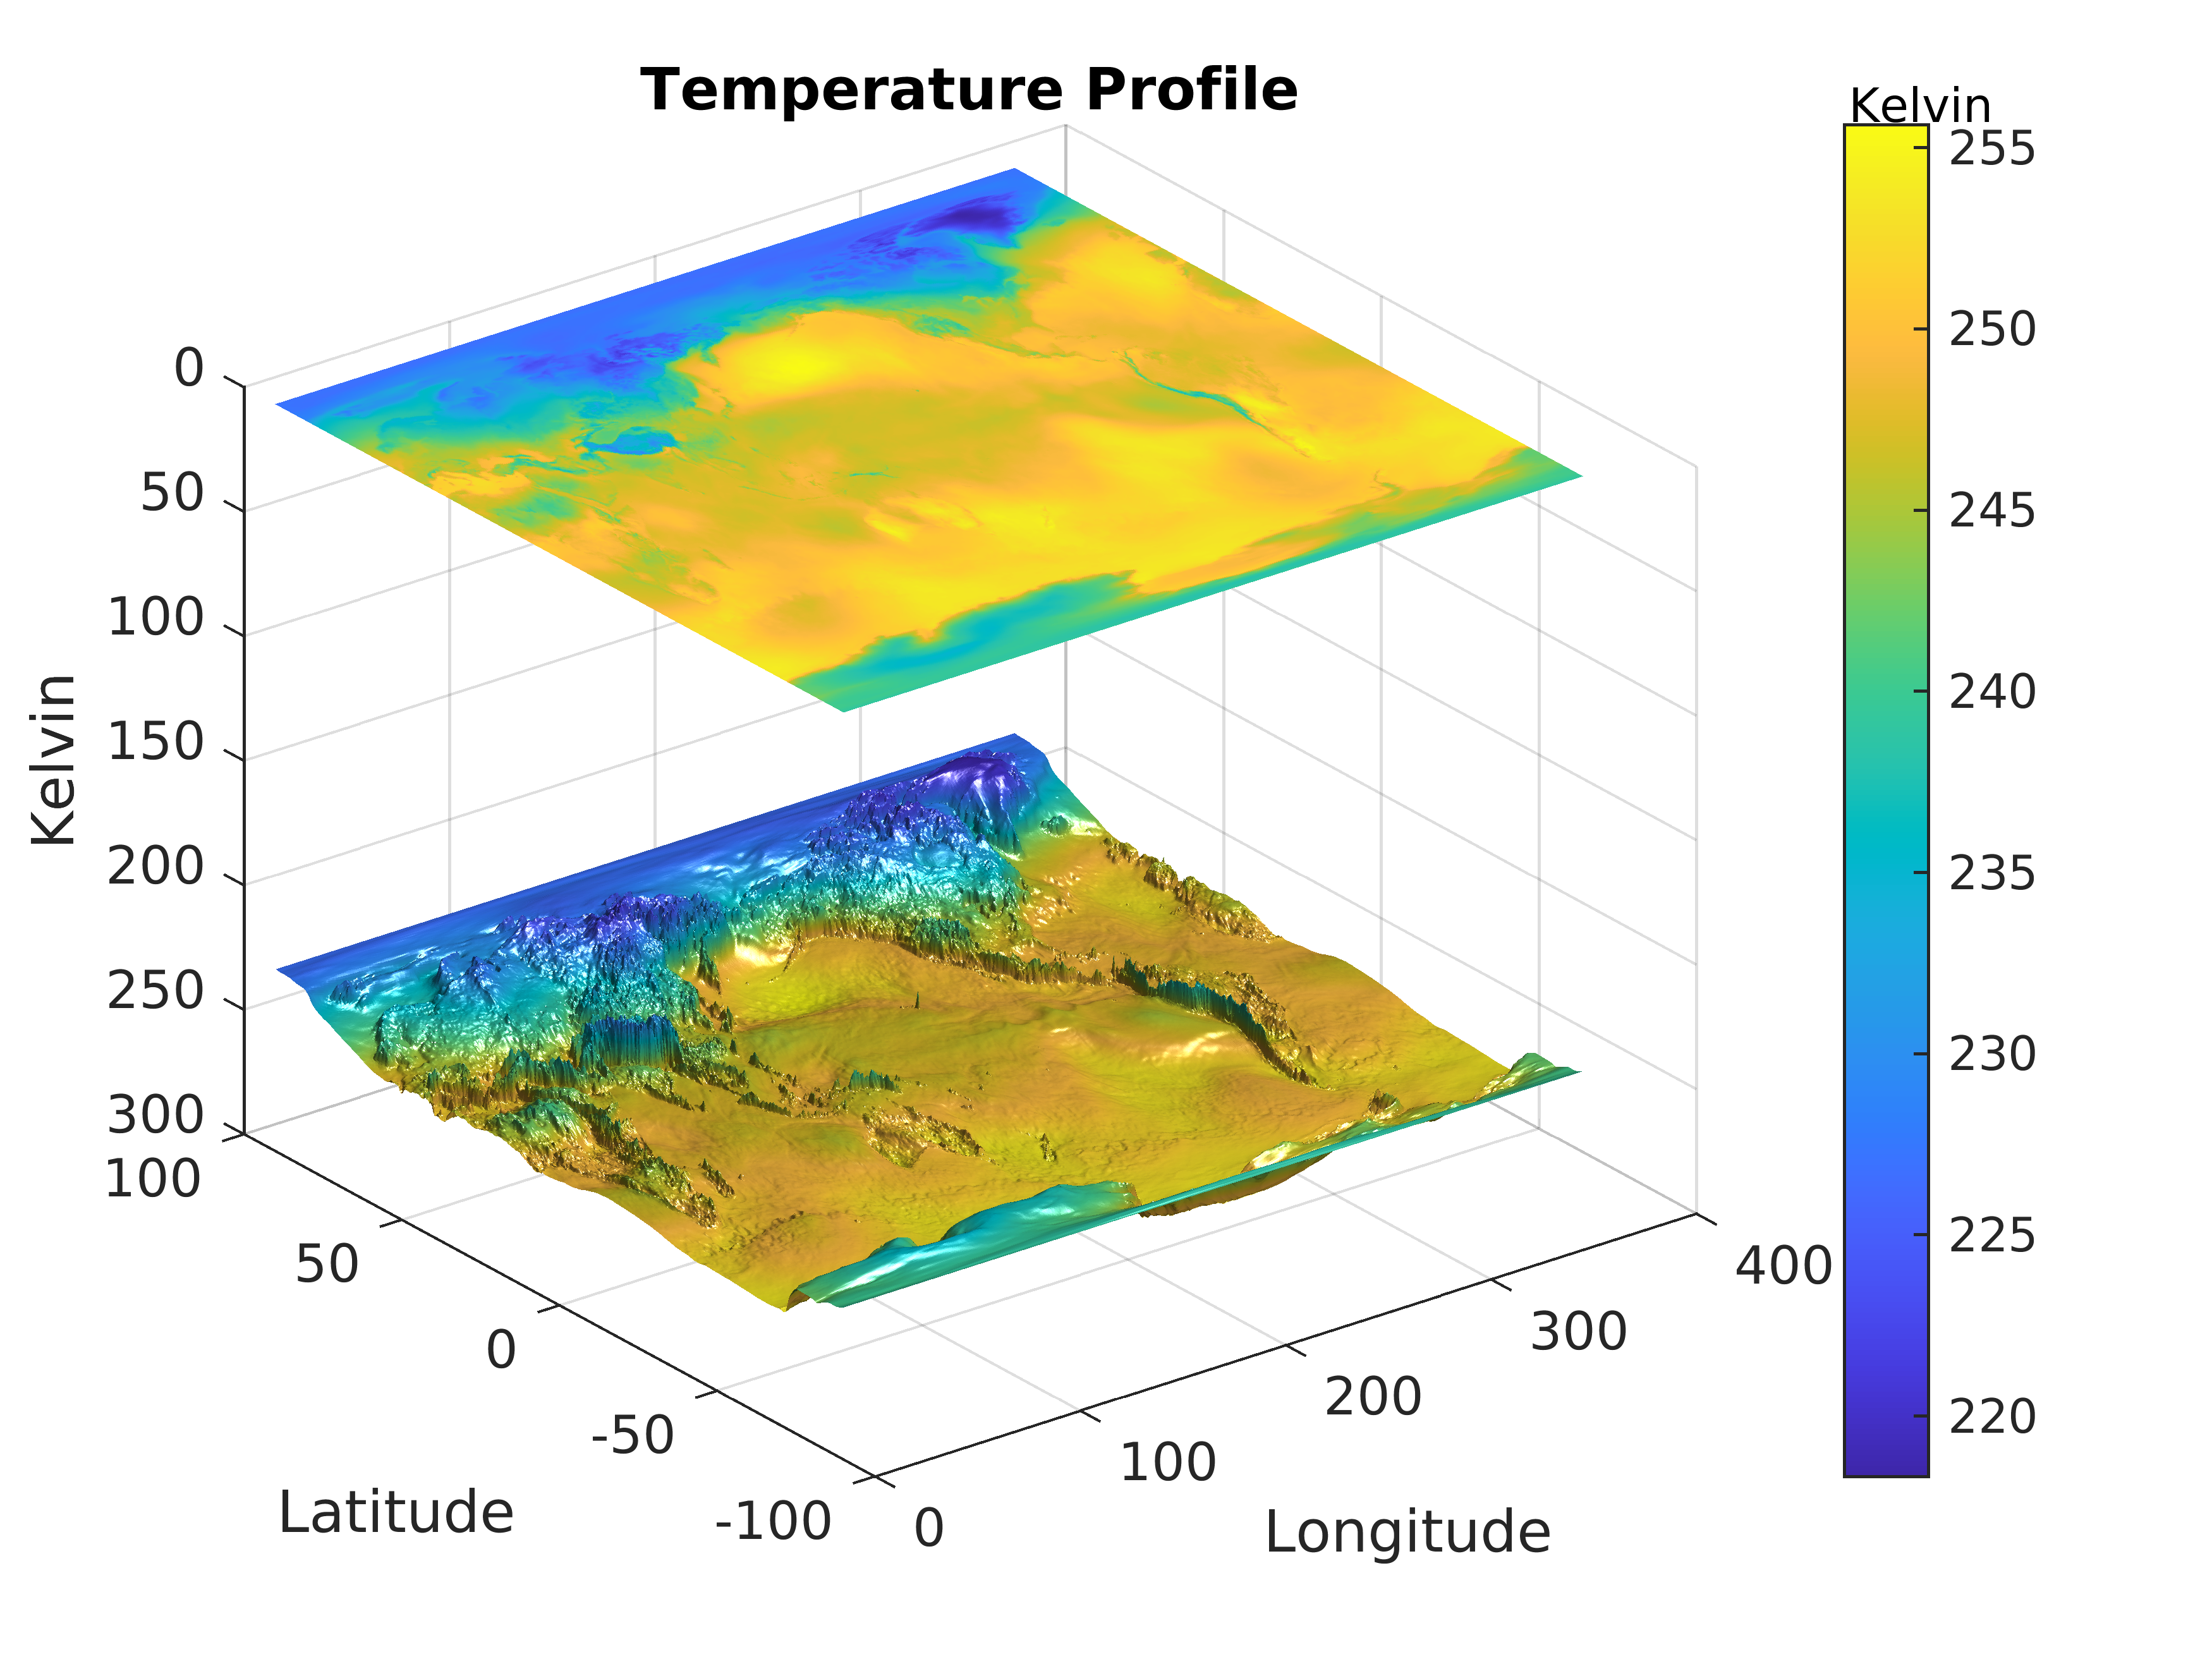
\includegraphics[width=\textwidth,clip=True,trim=0cm 0cm 1cm 0cm]{images/tempprof.png}
  \caption{Temperature profile\\ The top shows a flat pseudo-color\\ plot and the bottom shows a \\surface plot in degrees Kelvin. }
  \label{fig:subfig1}
\end{subfigure}%
\begin{subfigure}{0.5\textwidth}
  \centering
  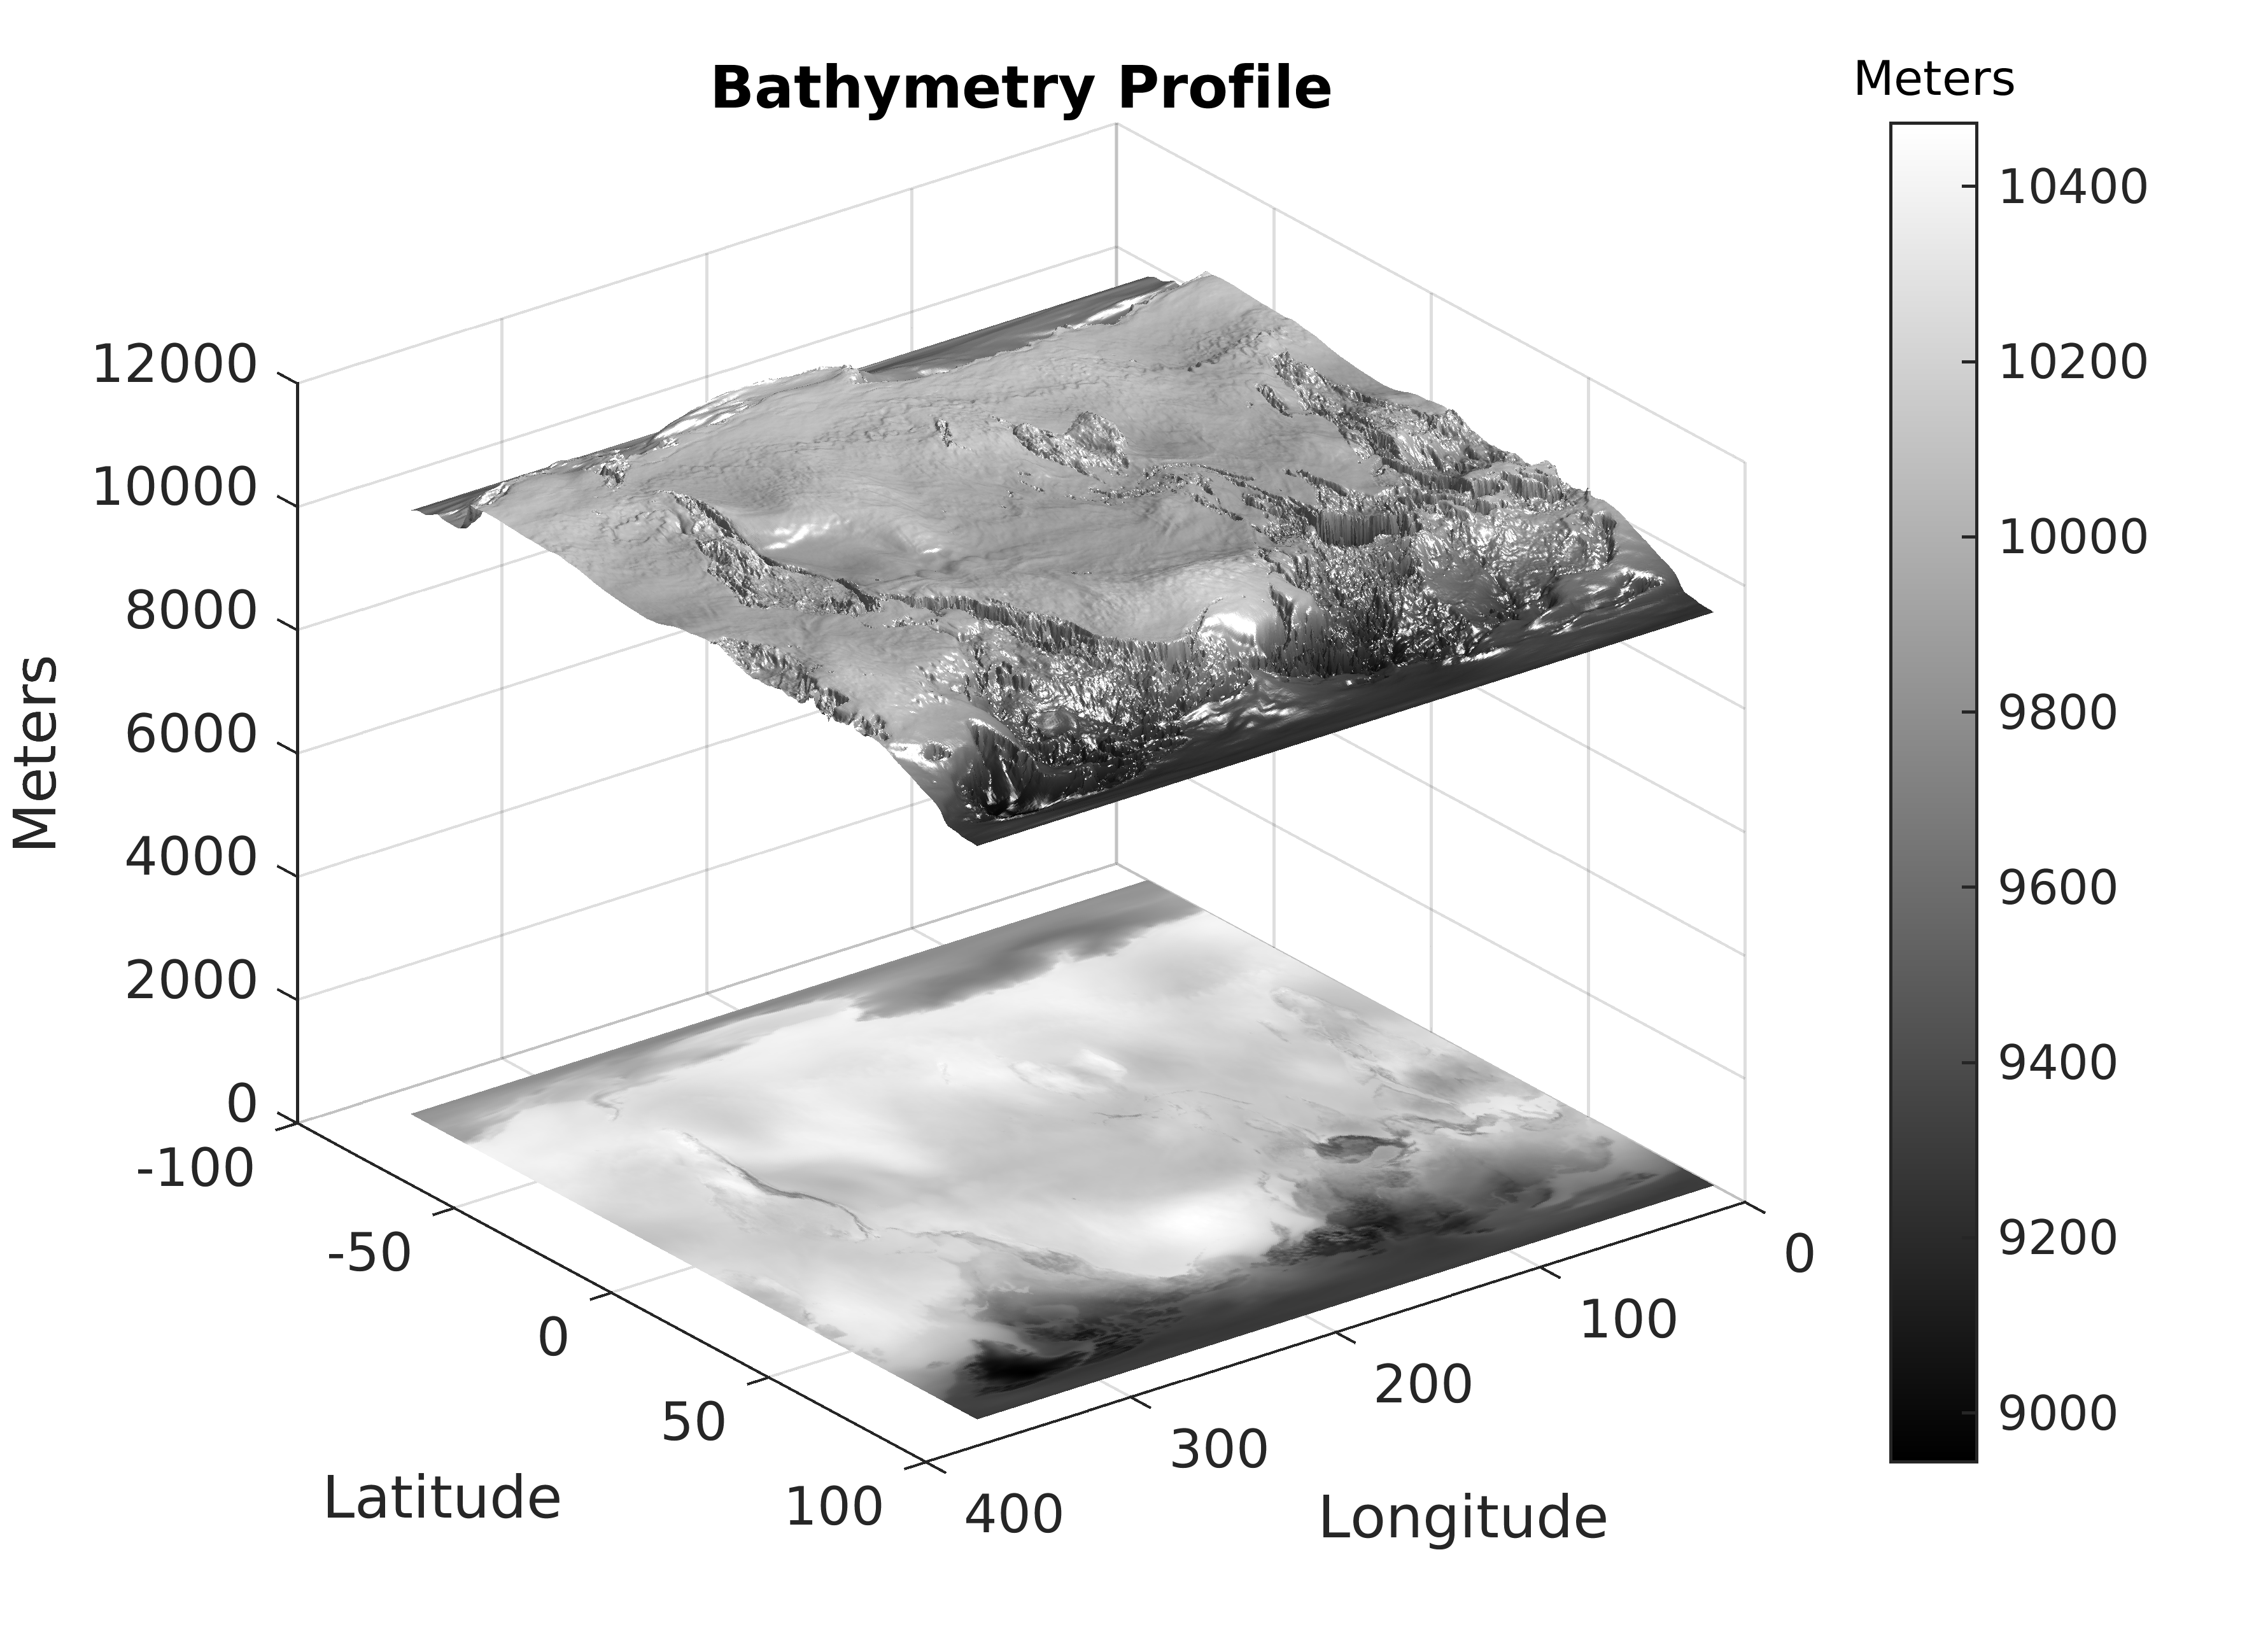
\includegraphics[width=\textwidth,clip=True,trim=0cm 0cm 1cm 0cm]{images/bathprof.png}
  \caption{Bathymetry Profile\\ The top shows the surface plot in meters and the bottom shows a flat pseudo-color plot.}
\end{subfigure}

\begin{subfigure}{\textwidth}
  \centering
     \centering
     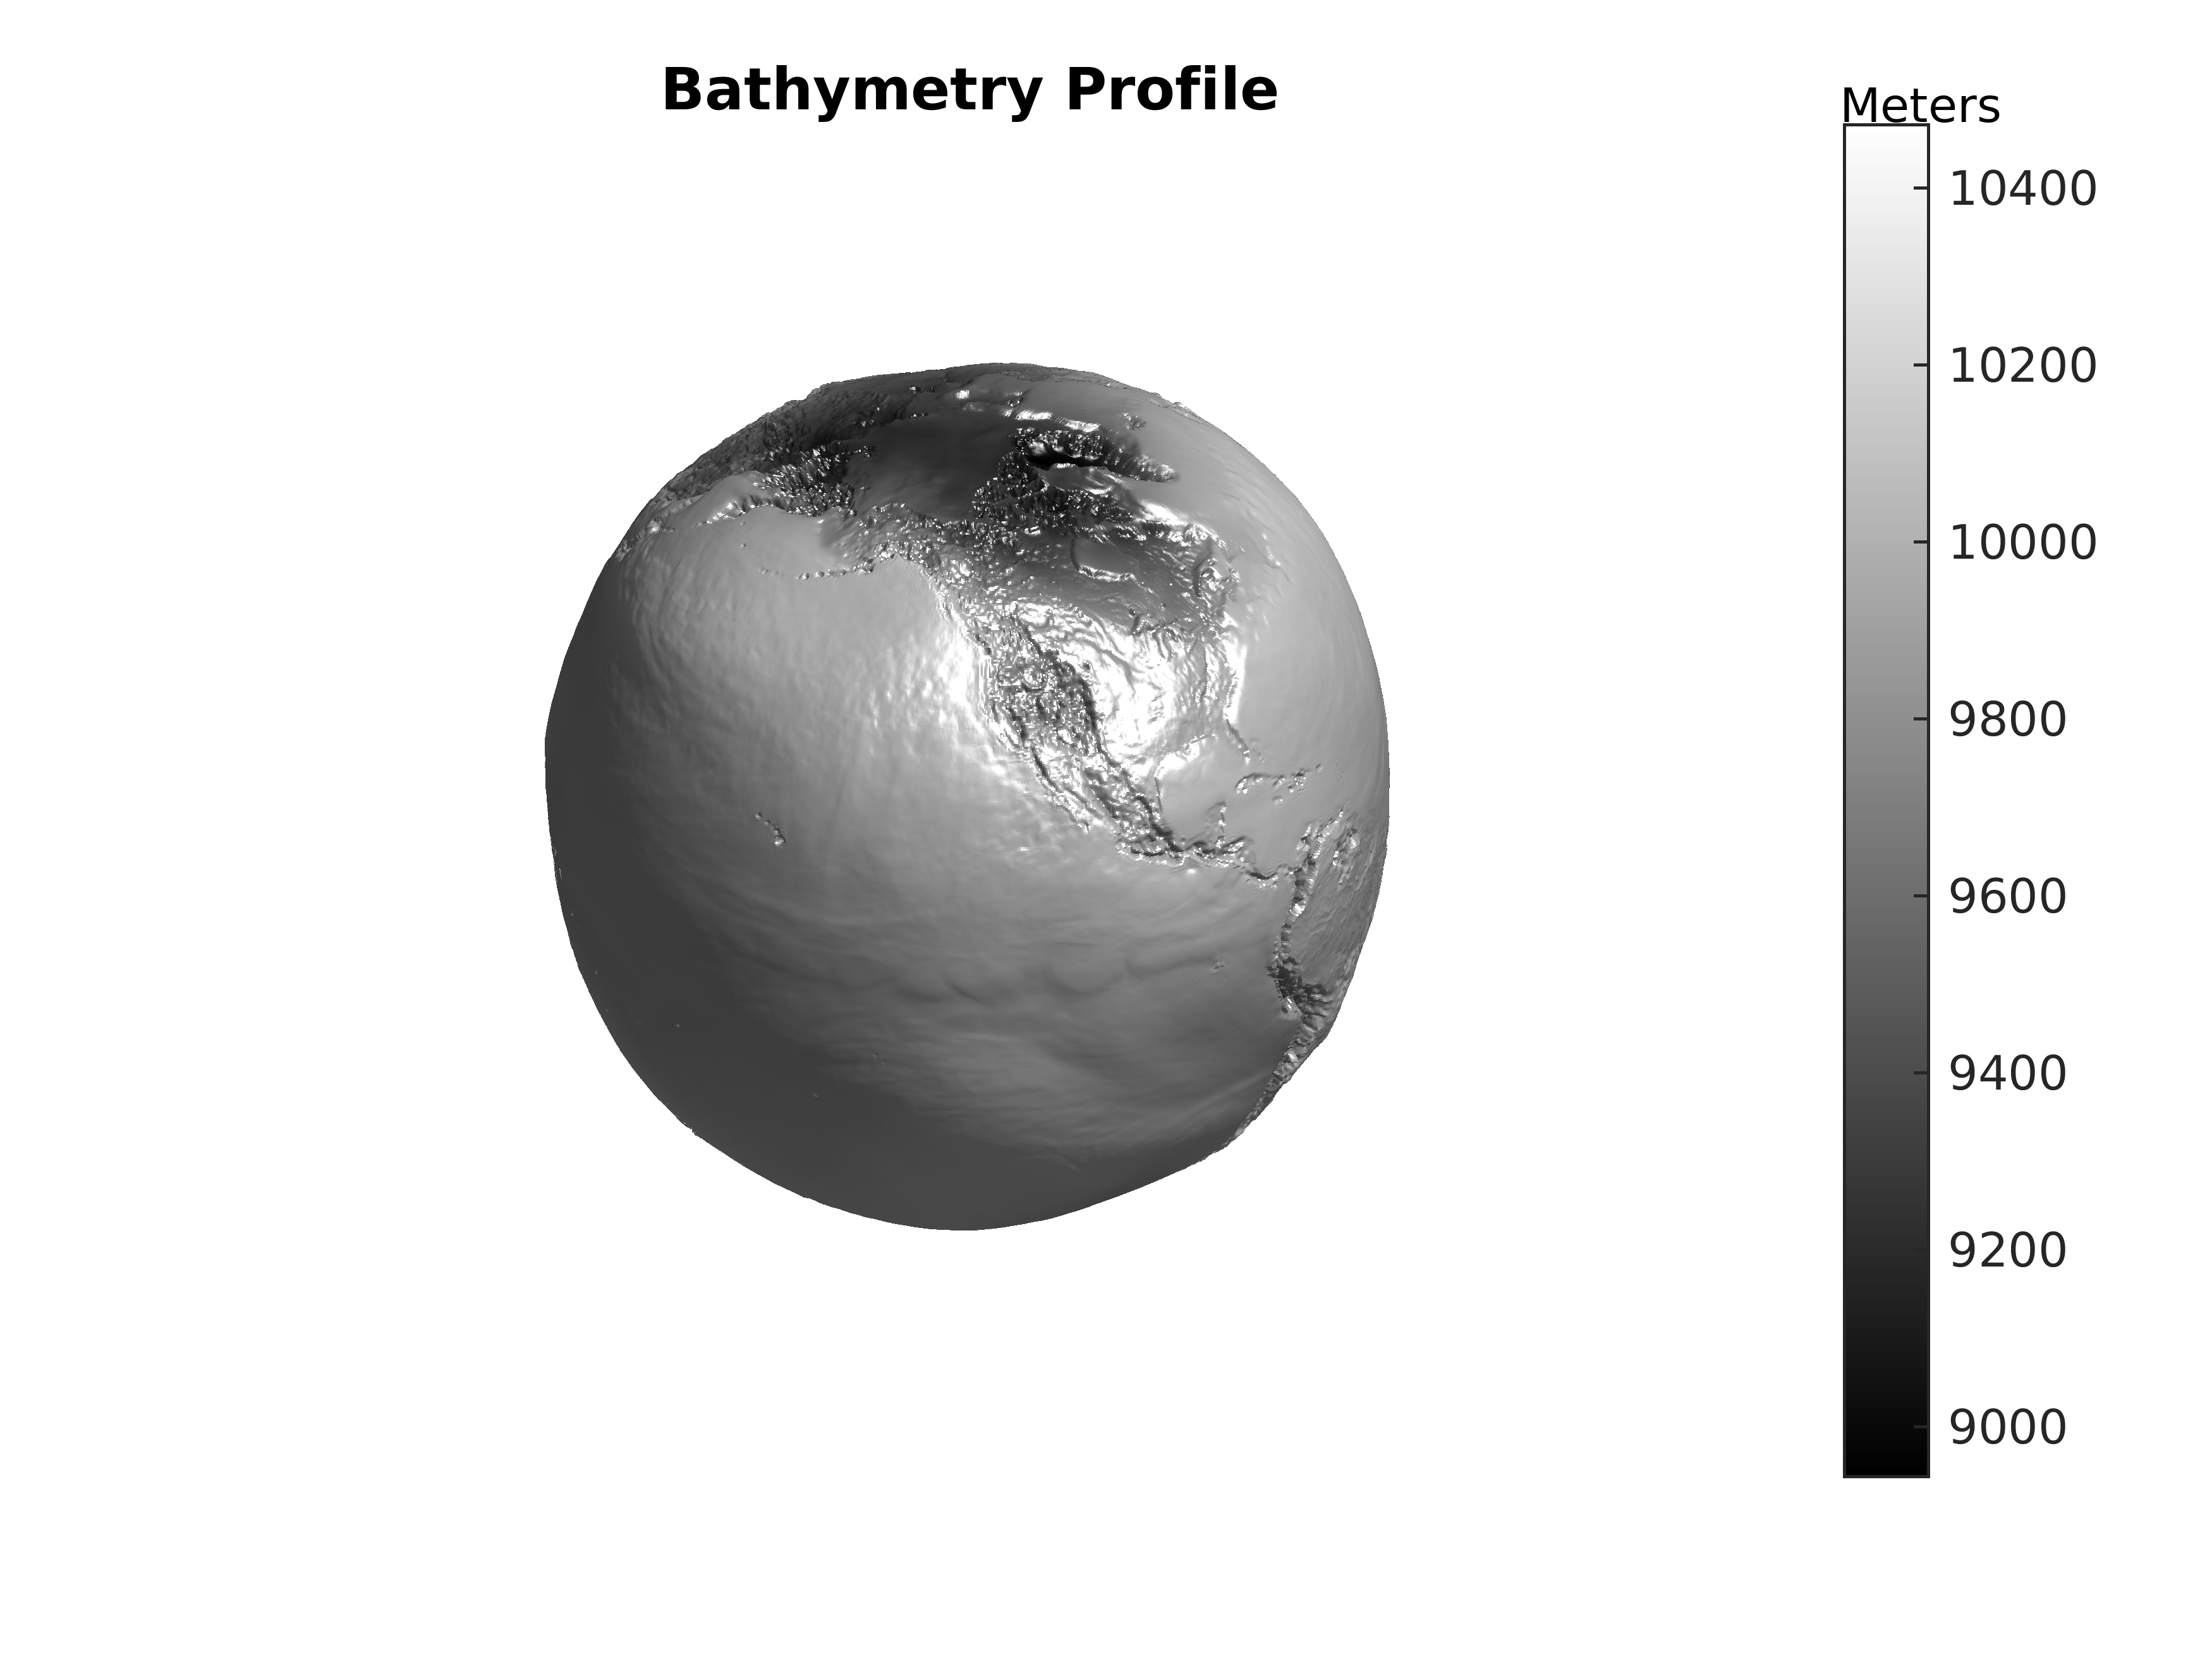
\includegraphics[width=0.5\textwidth,clip=True,trim=0cm 0cm 0cm 0cm]{images/bathprofglobe.png}
     \caption{Bathymetry on the globe}
\end{subfigure}
\caption{Averaged over 15 January 2022, 04:00 $\mathrm{UTC}$ - 21 January 2022, 04:00 $\mathrm{UTC}$}
\label{fig:4.3}
\end{figure}\\
 \indent The bathymetry data represents changes in flux relative to space, and so it acts as a source term
 \begin{equation}\label{eq:4.5}
	\begin{bmatrix}
		h\\
		hu\\
		hv\\
	\end{bmatrix}_{t}+\begin{bmatrix}
	uh\\
	hu^2+\frac{1}{2}gh^2\\
	uvh\\
\end{bmatrix}_{x}+\begin{bmatrix}
vh\\
uvh\\
hv^2+\frac{1}{2}gh^2\\
\end{bmatrix}_y=\begin{bmatrix}
    0\\
    -ghb_{x}\\
    -ghb_{y}\\
\end{bmatrix}
 \end{equation}
 The wave propagation algorithm mentioned previously in Section \ref{sec:2.3} can be modified to take this into account \cite{bale2003wave}. Since we are not considering that bathymetry changes with time we are only modifying the solution by a scalar value, and this can simply be incorporated into the Riemann solver as such.
 
 Some challenges remain in implementing this model, and this work will be carried out in a future project. However we can use the homogeneous solution present here to get a rough idea of idea of what the wave velocity with bathymetry might look like. From the data the maximum temperature was 321.5 $\mathrm{K}$ which translates to a bathymetry of 13169.3 $\mathrm{m}$. Also from the data the minimum temperature was 181.9 $\mathrm{K}$ which translates to a bathymetry of 7449.9 $\mathrm{m}$. Taking the average of these two bathymetry values we get an average bathymetry of 10309.6 $\mathrm{m}$. Figure \ref{fig:4.4} shows arrival of the wave at the half way point.
\begin{figure}[!htbp]
    \centering
    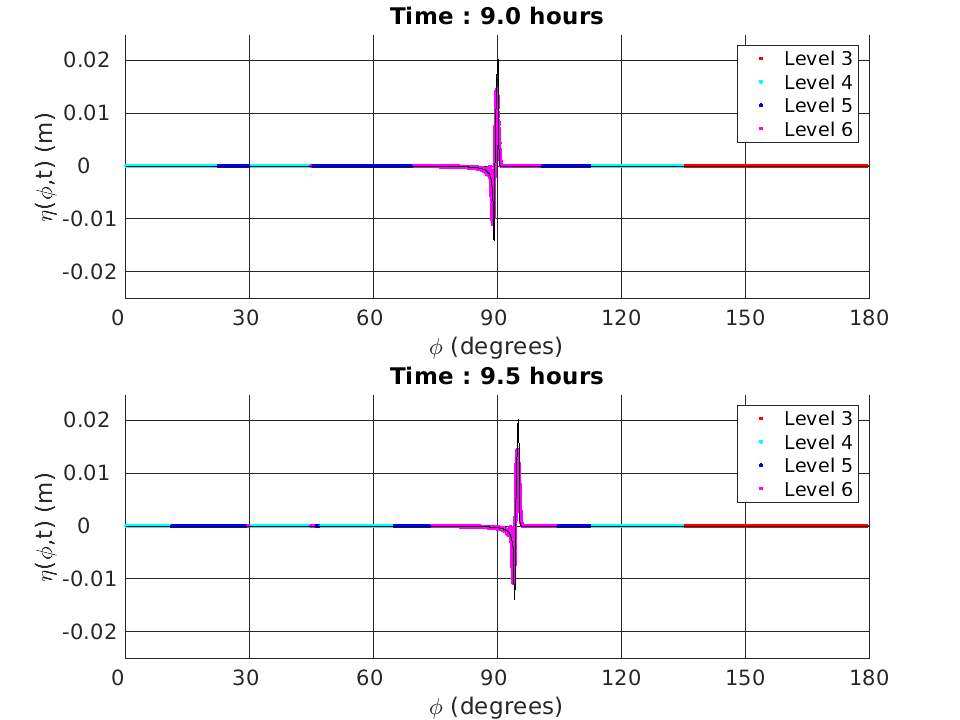
\includegraphics[width=\textwidth]{images/avgbath}
    \caption{Wave arrival at the half way point for the average bathymetry}
    \label{fig:4.4}
\end{figure}
Figure \ref{fig:4.5} shows the waves position for every half-hour time step.
\begin{figure}[!htbp]
    \centering
    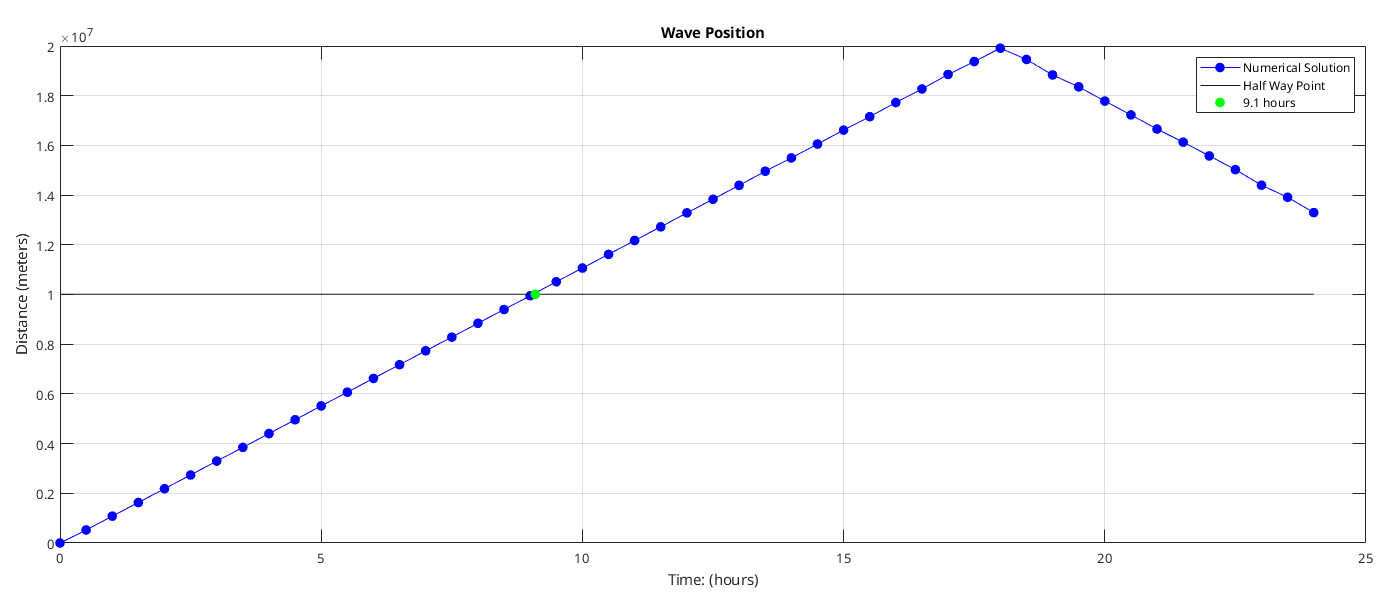
\includegraphics[width=\textwidth]{images/bathwavepos.png}
    \caption{Plot of distance versus time of traveling Lamb wave given the bathymetry.}
    \label{fig:4.5}
\end{figure}
Figure \ref{fig:4.6} shows the waves velocity for each half-hour time step and compares it to characteristic wave speed $c=\sqrt{gH}$ where $H=9.69$ $\mathrm{km}$.
\begin{figure}[!htbp]
    \centering
    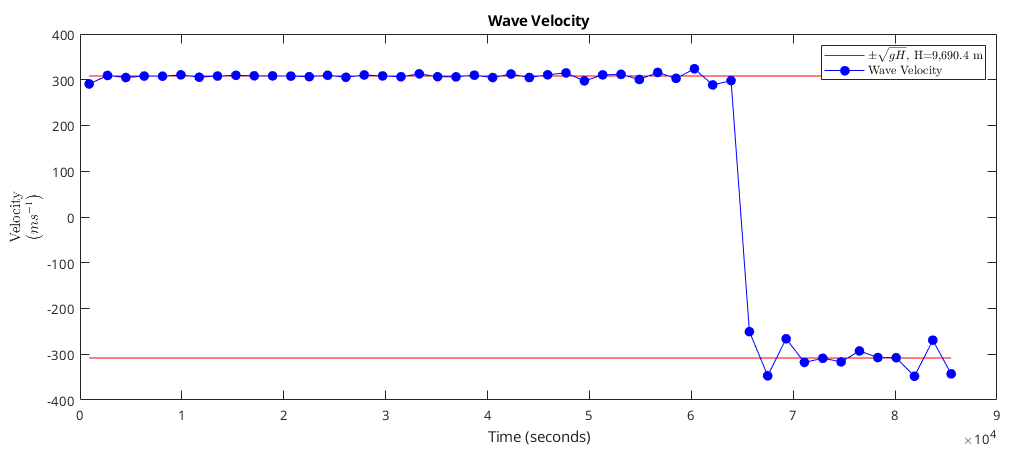
\includegraphics[width=\textwidth]{images/bathwavevelocity.png}
    \caption{Plot of the wave velocity versus time given the bathymetry. Also shown is characteristic speed $\sqrt{g H}$. }
    \label{fig:4.6}
\end{figure}
The wave arrives at the half way point at around 9.1 hours and traveling at a velocity of 309.2 $\mathrm{ms}^{-1}$. Note that the velocity of the wave scaled for the average bathymetry is very close to the theoretical speed of Lamb waves. This demonstrates that incorporating temperature into our model we may get a result that is better match for the sensor data and the results of the model that Amores et al. \cite{amores2022numerical} produced.
%%%%%%%%%%%%%%%%%%%%%%%%%%%%%%%%%%%%%%%%%%%%%%%%%%%%%%%%%%%%%%%%%%%%%%%%%%%%%%
%
% Chapter: Conclusion
%
%%%%%%%%%%%%%%%%%%%%%%%%%%%%%%%%%%%%%%%%%%%%%%%%%%%%%%%%%%%%%%%%%%%%%%%%%%%%%%
\chapter{Conclusion}
The 2022 Hunga Tonga-Hunga Ha’apai eruption released a large amount of energy into earth's atmosphere causing disturbances that propagated like Lamb waves. Previous works have modeled the waves generated by the eruption as a shallow water system. Here we have modeled these waves similarly using high resolution finite volume methods, and demonstrated that the homogeneous shallow water equations at earth scale produce reasonably good results with these methods. We have also demonstrated incorporating temperature as bathymetry would produce a much more accurate model. In future work we will incorporate temperature variations present in the atmosphere to produce a more advanced model.
\backmatter

%%%%%%%%%%%%%%%%%%%%%%%%%%%%%%%%%%%%%%%%%%%%%%%%%%%%%%%%%%%%%%%%%%%%%%%%%%%%%%
%
% References
%
%%%%%%%%%%%%%%%%%%%%%%%%%%%%%%%%%%%%%%%%%%%%%%%%%%%%%%%%%%%%%%%%%%%%%%%%%%%%%%

\bibliographystyle{plain}

\label{references}

\bibliography{Bibliography}

%%%%%%%%%%%%%%%%%%%%%%%%%%%%%%%%%%%%%%%%%%%%%%%%%%%%%%%%%%%%%%%%%%%%%%%%%%%%%%
%
% Appendix
%
%%%%%%%%%%%%%%%%%%%%%%%%%%%%%%%%%%%%%%%%%%%%%%%%%%%%%%%%%%%%%%%%%%%%%%%%%%%%%%

% Use the \appendix command (only once) to start the appendix (or appendices)

%\appendix

% After \appendix has executed, the \chapter command creates an appendix.
% Appendices are numbered by "A", "B", etc.

%\chapter{Appendix Name A}\label{app:appendixA}

%\chapter{Appendix Name B}\label{app:appendixB}


% The \finish command is executed just before the \end{document}. 
% Among other things, it produces the requisite blank page at the end
% of the document.
\finish

\end{document}